\documentclass[12pt, a4paper, final, oneside]{report}

\newcommand{\isPrintVersion}{false}						% false -> show colored links, true -> all links in black

\usepackage[utf8]{inputenc}
%%%%%%%%%%%%%%%%%%%%%%%%%%%%%%%%%%%%%%%%%%%%%%%%%%%%%%%%%%%%%%%%%%%%%%%%%%%%%%%%
%%%%%%%%%%%%%%%%%%%%%%%%%%%%%%% Data  %%%%%%%%%%%%%%%%%%%%%%%%%%%%%%%%%%%%%%%%%%
\newcommand{\reportTitle}{Erweiterung des SPMS um ein Weekly Standup Modul}
\newcommand{\authorName}{Julia Heydecke, Christine Kuczera, Hicham Naoufal, Samuel Pliska, Ivo Valls}
\newcommand{\reportDate}{15. Juli 2022}

%%%%% Title page
\newcommand{\reportType}{Projektbericht}
\newcommand{\courseOfStudies}{Projektmanagement}
\newcommand{\university}{Berliner Hochschule für Technik}

\newcommand{\timeOfProject}{SS2022}
\newcommand{\studentId}{1234567}
\newcommand{\course}{XYZ1234}

\newcommand{\supervisorName}{Prof. Dr. Glißmann-Hochstein}


\newcommand{\byTitle}{von}
\newcommand{\courseOfStudiesTitle}{Course of Studies}
\newcommand{\timeOfProjectTitle}{Durfgeführt im}
\newcommand{\studentIdTitle}{Durchgeführt von}
\newcommand{\supervisorTitle}{Bei Dozentin}



\newcommand{\ListOfFiguresTitle}{Abbildungsverzeichnis}
\newcommand{\ListOfAbbreviationsTitle}{Abkürzungsverzeichnis}
\newcommand{\ListOfTablesTitle}{Tabellenverzeichnis}
\newcommand{\ListOfListingsTitle}{Quellcodeverzeichnis}

%%%%% Document
\title{\reportTitle}
\author{\authorName}

%%%%%%%%%%%%%%%%%%%%%%%%%%%%%%%%%%%%%%%%%%%%%%%%%%%%%%%%%%%%%%%%%%%%%%%%%%%%%%%%
%%%%%%%%%%%%%%%%%%%%%%%%%%%%%%%% Abstract  %%%%%%%%%%%%%%%%%%%%%%%%%%%%%%%%%%%%%
\usepackage{abstract}
\renewcommand{\abstractnamefont}{\large\bfseries}


%%%%%%%%%%%%%%%%%%%%%%%%%%%%%%%%%%%%%%%%%%%%%%%%%%%%%%%%%%%%%%%%%%%%%%%%%%%%%%%%
%%%%%%%%%%%%%%%%%%%%%%%%%%%%%%%% Packages  %%%%%%%%%%%%%%%%%%%%%%%%%%%%%%%%%%%%%
\usepackage[left=3cm,right=3cm,top=3cm,bottom=3cm]{geometry}
\usepackage[ngerman]{babel}
\usepackage{amsmath}
\usepackage{amsfonts}
\usepackage{amssymb}
\usepackage{enumitem}
\usepackage{float}
\usepackage{fancyhdr}
\usepackage[bottom]{footmisc}
\usepackage[printonlyused]{acronym}
\usepackage{appendix}
\usepackage{pdfpages}
\usepackage{ifthen}
\usepackage{csquotes}
\usepackage{emptypage}

%%%%%%%%%%%%%%%%%%%%%%%%%%%%%%%%%%%%%%%%%%%%%%%%%%%%%%%%%%%%%%%%%%%%%%%%%%%%%%%%
%%%%%%%%%%%%%%%%%%%%%%%%%%%%%% Colors  %%%%%%%%%%%%%%%%%%%%%%%%%%%%%%%%%%%%%%%%%
\definecolor{darkBlue}{cmyk}{0.9592, 0.4592, 0, 0.6157} % {HTML}{043562}
\definecolor{lightBlue}{cmyk}{0.5, 0.25, 0, 0.2} 		% {HTML}{6699cc}
\definecolor{darkGrey}{cmyk}{0, 0, 0, 0.9333} 			% {HTML}{111111}
\definecolor{lightGrey}{cmyk}{0.0164, 0.0082, 0, 0.0431}% {HTML}{F0F2F4}
\definecolor{magenta}{cmyk}{0, 1, 0.4972, 0.3059}		% {HTML}{B10059}

%%%%%%%%%%%%%%%%%%%%%%%%%%%%%%%%%%%%%%%%%%%%%%%%%%%%%%%%%%%%%%%%%%%%%%%%%%%%%%%%
%%%%%%%%%%%%%%%%%%%%%%%%%%%%%% New commands  %%%%%%%%%%%%%%%%%%%%%%%%%%%%%%%%%%% 

%%%%% Caption with sources
\usepackage{caption}
\captionsetup{justification=centering}
\newcommand{\captionsource}[2][]{
	\ifthenelse{\equal{#1}{}}
		{\small\textit{Source: #2}} % if empty
		{\small\textit{Source: #2, \href{#1}{#1}} % else
	}
}

%%%%% Theorems / Definitions
\usepackage{amsthm} 					
\newtheorem{define}{Definition}

%%%%% Code in text
\newcommand{\code}[1]{{\ttfamily#1}}

%%%%%%%%%%%%%%%%%%%%%%%%%%%%%%%%%%%%%%%%%%%%%%%%%%%%%%%%%%%%%%%%%%%%%%%%%%%%%%%%
%%%%%%%%%%%%%%%%%%%%%%%%%%%%%% Bibliography  %%%%%%%%%%%%%%%%%%%%%%%%%%%%%%%%%%%
\usepackage[backend=bibtex,style=numeric,citestyle=numeric]{biblatex}
\bibliography{bibliography} 

% linebreaks in bibliography urls
\usepackage{url}
\usepackage{breakurl}
\def\UrlBreaks{\do\/\do-}							% add a breakpoint at - and /

\setcounter{biburlnumpenalty}{1000}  				% add a breakpoint after all numbers
\setcounter{biburlucpenalty}{1000}					% add a breakpoint after all uppercase letters
\setcounter{biburllcpenalty}{1000}   				% add a breakpoint after all lowercase letters

%%%%%%%%%%%%%%%%%%%%%%%%%%%%%%%%%%%%%%%%%%%%%%%%%%%%%%%%%%%%%%%%%%%%%%%%%%%%%%%%
%%%%%%%%%%%%%%%%%%%%%%%%%%%%%%% PDF settings  %%%%%%%%%%%%%%%%%%%%%%%%%%%%%%%%%%
\usepackage[pdftitle={\reportTitle}, pdfauthor={\authorName},pdfsubject={\reportTitle}, pdfcreator={pdflatex}, pdfpagemode=UseOutlines, pdfdisplaydoctitle=true, pdflang={en}, breaklinks]{hyperref}

% color settings for links in pdf
\ifthenelse{\equal{\isPrintVersion}{true}}
{ % print version
	\hypersetup{
		hidelinks=true,
		colorlinks=false, 
		linktocpage=true, 							% page numbers are clickable
		bookmarksnumbered=true 						% show heading numbering in pdf table of contents
	}
}{ % screen version
	\hypersetup{
		colorlinks=true, 
		linkcolor=darkBlue,
		citecolor=darkBlue,
		filecolor=darkBlue,
		menucolor=darkBlue,
		urlcolor=darkBlue,
		linktocpage=true, 							% page numbers are clickable
		bookmarksnumbered=true 						% show heading numbering in pdf table of contents
	}
}

%%%%%%%%%%%%%%%%%%%%%%%%%%%%%%%%%%%%%%%%%%%%%%%%%%%%%%%%%%%%%%%%%%%%%%%%%%%%%%%%
%%%%%%%%%%%%%%%%%%%%%%%%%%%%%%% Typography  %%%%%%%%%%%%%%%%%%%%%%%%%%%%%%%%%%%%
\usepackage{lmodern}
\usepackage{mathpazo}
\fontfamily{ppl}\selectfont

\setlength{\parskip}{8pt}							% after paragraph
\setlength{\parindent}{0pt}							% new paragraph indent
\renewcommand{\baselinestretch}{1.2}\normalsize		% line height (line height for content is defined in line 281)

% Prevent widows and orphans
\clubpenalty = 10000								% prevent orphans
\widowpenalty = 10000 								% prevent widows
\displaywidowpenalty=10000

% Headings
\usepackage{titlesec}
\newcommand{\hsp}{\hspace{20pt}}

\titleformat{\chapter}[block]{\Huge\bfseries}{\thechapter \hsp {|}\hsp}{0pt}{\Huge\bfseries}
\titleformat{\section}[block]{\Large\bfseries}{\thesection \ }{0pt}{\Large \bfseries}
\titleformat{\subsection}[block]{\large\bfseries}{\thesubsection \ }{0pt}{\large \bfseries}
%%%%%%%%%%%%%%%%%%%%%%%%%%%%%%%%%%%%%%%%%%%%%%%%%%%%%%%%%%%%%%%%%%%%%%%%%%%%%%%%
%%%%%%%%%%%%%%%%%%%%%%%%%%%%%%%%%%% Listings  %%%%%%%%%%%%%%%%%%%%%%%%%%%%%%%%%%
\usepackage{listings}

\lstset{
	language=Java,								% default language
	numbers=left,								% line number position, alternative: none
	stepnumber=1,								 
	numbersep=6pt,								% distance between line number and code
	numberstyle=\fontsize{9pt}{9pt}\ttfamily,	% line number style
	breaklines=true,							% break lines if necessary
	breakautoindent=true,						% indent after line break
	postbreak=\space,							% break at space
	tabsize=4,									% tab size
	showspaces=false,							% do not show spaces in code
	showstringspaces=false,						% do not show spaces in strings
	extendedchars=true,							% use Latin1
	captionpos=b,								% caption position
	backgroundcolor=\color{lightGrey}, 			% background color
	xleftmargin=0pt,								
	xrightmargin=0pt,							
	frame=leftline,								% draw frame ar left side only
	framerule=1.1pt,							% frame width
	frameround=ffff,							% round corners: f = not rounded | t = rounded
	rulecolor=\color{lightBlue},				% frame color
	framesep=1.5pt,								% distance between line number and border 
	fillcolor=\color{lightGrey},
	basicstyle=\ttfamily\footnotesize\color{darkGrey},	
	keywordstyle=\color{magenta}\bfseries,
	identifierstyle=,
	commentstyle=\color{lightBlue},
	stringstyle=\color{darkBlue}
}

\lstloadlanguages{bash, C, C++, HTML, Java, PHP, Python, SQL}

% change heading above listings to \ListOfListingsTitle
\renewcommand{\lstlistlistingname}{\ListOfListingsTitle}

% Group list of listings by chapter
\let\Chapter\chapter
\def\chapter{\addtocontents{lol}{\protect\addvspace{10pt}}\Chapter}

%%%%%%%%%%%%%%%%%%%%%%%%%%%%%%%%%%%%%%%%%%%%%%%%%%%%%%%%%%%%%%%%%%%%%%%%%%%%%%%%
%%%%%%%%%%%%%%%%%%%%%%%%%%%%%%%%%%% Images  %%%%%%%%%%%%%%%%%%%%%%%%%%%%%%%%%%
\graphicspath{
    {images/}
	{plots/}
}

%%%%%%%%%%%%%%%%%%%%%%%%%%%%%%%%%%%%%%%%%%%%%%%%%%%%%%%%%%%%%%%%%%%%%%%%%%%%%%%%
%%%%%%%%%%%%%%%%%%%%%%%%%%%%%%%%%%% Diagrams  %%%%%%%%%%%%%%%%%%%%%%%%%%%%%%%%%%
\usepackage{tikz}
\usetikzlibrary{shapes,arrows,shadows}
% flow diagrams
\tikzstyle{startstop} = [rectangle, rounded corners, minimum width=3cm, minimum height=0.9cm,text centered, draw=lightBlue, fill=lightGrey]
\tikzstyle{io} = [trapezium, trapezium left angle=70, trapezium right angle=110, minimum width=3cm, minimum height=0.9cm, text centered, draw=lightBlue, fill=lightGrey]
\tikzstyle{process} = [rectangle, minimum width=3cm, minimum height=0.9cm, text centered, text width=3cm, draw=lightBlue, fill=lightGrey]
\tikzstyle{decision} = [diamond, minimum width=3cm, minimum height=0.9cm, text centered, draw=lightBlue, fill=lightGrey]
\tikzstyle{arrow} = [thick,->,>=stealth]
\tikzstyle{comment} = [rectangle, minimum width=1cm, minimum height=0.9cm, text centered, text width=3cm, draw=none, fill=none]
\tikzstyle{subprocess} = [rectangle split, rectangle split horizontal, rectangle split parts=3, minimum height=0.9cm, minimum width=3cm, draw=lightBlue, fill=lightGrey]

% sequence diagrams
\usepackage[underline=false]{pgf-umlsd}

%%%%%%%%%%%%%%%%%%%%%%%%%%%%%%%%%%%%%%%%%%%%%%%%%%%%%%%%%%%%%%%%%%%%%%%%%%%%%%%%
%%%%%%%%%%%%%%%%%%%%%%%%%%%%% Todo Comments  %%%%%%%%%%%%%%%%%%%%%%%%%%%%%%%%%%%
\usepackage[colorinlistoftodos]{todonotes}
\reversemarginpar
\setlength{\marginparwidth}{3cm}

\newcommand{\todoQuestion}[1]{\todo[color=green!40]{#1}}
\newcommand{\todoImportant}[1]{\todo[color=red!60]{#1}}

%%%%%%%%%%%%%%%%%%%%%%%%%%%%%%%%%%%%%%%%%%%%%%%%%%%%%%%%%%%%%%%%%%%%%%%%%%%%%%%%
%%%%%%%%%%%%%%%%%%%%%%%%%%%%%%%%%% Structure  %%%%%%%%%%%%%%%%%%%%%%%%%%%%%%%%%%
\begin{document}
	\setlength{\headheight}{24.7pt}					% minimum height required by Latexmk
	\pagenumbering{Roman}

%%%%% Title page, quote, declaration, abstract 
	\fancypagestyle{plain}{ 						% no header, no footer
		\fancyhf{} 
		\fancyfoot{}
		\renewcommand{\headrulewidth}{0pt}
		\renewcommand{\footrulewidth}{0pt}
	}	
	\begin{titlepage}	
	\centering
	
	{\large \ \par}
	{\scshape\LARGE \reportType \par}	
	\vspace{1.5cm}
	{\huge\bfseries \reportTitle \par}
	\vspace{1.5cm}
	{\large \courseOfStudies \\ an der \university \par}
	\vspace{1cm}
	{\large \byTitle \par}
	{\Large\itshape \authorName \par}
	\vfill
	{\large \reportDate \par}
	\vfill
	\begin{tabbing}
		mmmmmmmmmmmmmmmmmmmmmmmmmm			\= \kill 			% define width
		\textbf{\timeOfProjectTitle}		\> \timeOfProject \\
		\textbf{\studentIdTitle}			\> Julia Heydecke \\
											\> Christine Kuczera \\
											\> Hicham Naoufal \\
											\> Samuel Pliska\\
											\> Ivo Valls \\
		\textbf{\supervisorTitle}			\> \supervisorName \\		
	\end{tabbing}
\end{titlepage}




	\cleardoublepage
\begin{otherlanguage}{ngerman} 
\begin{abstract}
Dies ist ein Typoblindtext. An ihm kann man sehen, ob alle Buchstaben da sind und wie sie aussehen. Manchmal benutzt man Worte wie Hamburgefonts, Rafgenduks oder Handgloves, um Schriften zu testen. Manchmal Sätze, die alle Buchstaben des Alphabets enthalten - man nennt diese Sätze Pangrams. Sehr bekannt ist dieser: The quick brown fox jumps over the lazy old dog.

Oft werden in Typoblindtexte auch fremdsprachige Satzteile eingebaut (AVAIL® and Wefox™ are testing aussi la Kerning), um die Wirkung in anderen Sprachen zu testen. In Lateinisch sieht zum Beispiel fast jede Schrift gut aus. Quod erat demonstrandum. Seit 1975 fehlen in den meisten Testtexten die Zahlen, weswegen ab dem Jahr 2034 Zahlen in 86 der Texte zur Pflicht werden.

Nichteinhaltung wird mit bis zu 245 Euro oder 368 bestraft. Genauso wichtig in sind mittlerweile auch Âçcèñtë, die in neueren Schriften aber fast immer enthalten sind. Ein wichtiges aber schwierig zu integrierendes Feld sind OpenType-Funktionalitäten. Je nach Software und Voreinstellungen können eingebaute Kapitälchen, Kerning oder Ligaturen (sehr pfiffig) nicht richtig dargestellt werden.
\end{abstract}
\end{otherlanguage}


%%%%% Table of Contents
	\setlength{\parskip}{0pt}						% after paragraph
	\setcounter{tocdepth}{1}						% depth of table of contents
	\tableofcontents
	\thispagestyle{empty}
		
%%%%% Figures, Tables, Listings	
	\fancypagestyle{plain}{ 
		\fancyhf{} 
		\fancyfoot[R]{\thepage}
		\renewcommand{\headrulewidth}{0pt}
		\renewcommand{\footrulewidth}{0pt}
	}	
	\addtocounter{page}{3}							% increase page number: +6
	% only used acronyms are displayed
% \ac{LOL}  -> First time: Laughing Out Loud (LOL), Else: LOL
% \acs{LOL} -> LOL
% \acf{LOL} -> Laughing Out Loud (LOL)
% \acs{LOL} -> Laughing Out Loud
% \acp{LOL} -> LOLs
% documentation: https://www.ctan.org/pkg/acronym

\chapter*{Abkürzungsverzeichnis}

\begin{acronym}[AABBCCD]  			% define width of left column 
\setlength{\itemsep}{-\parsep}			% define spacing between acronyms

\acro{SPMS}{Student Project Management System}
\acro{MCI}{Mensch Computer Interaktion}
\end{acronym}

	\addcontentsline{toc}{chapter}{\ListOfAbbreviationsTitle}		

	\listoffigures
	\addcontentsline{toc}{chapter}{\ListOfFiguresTitle}	

	%\cleardoublepage
	\listoftables
	\addcontentsline{toc}{chapter}{\ListOfTablesTitle}	
	
	\lstlistoflistings
	\addcontentsline{toc}{chapter}{\ListOfListingsTitle}

	\cleardoublepage

%%%%% Content
	\pagenumbering{arabic}
	\setlength{\parskip}{8pt}						% after paragraph
	\renewcommand{\baselinestretch}{1.4}\normalsize	% line height 
	
	\pagestyle{fancy}
	\fancyhf{}
	\renewcommand{\chaptermark}[1]{\markboth{#1}{}}
	\fancyhead[R]{\thechapter  \ -- \ \nouppercase\leftmark}
	\fancyfoot[R]{\thepage}
	\chapter{Einführung}

Zielsetzung unseres Teams (DEV-2) war gemeinsam ein Feature umfänglich für das \ac{SPMS} zu entwickeln. Nach einem initialen Brainstorming haben wir uns für die Entwicklung eines Weekly Standup Moduls entschieden. Hierzu haben wir zuerst eine Marktanalyse durchgeführt, um zu eruieren, welche Features bereits am Markt vorhanden sind. In einem nächsten Schritt haben wir uns überlegt, wer unser Zielnutzer sein werden und haben auf dieser Grundlage Personas erstellt. Davon ausgehend haben wir Interviews mit potenziellen Nutzern geführt, um ein besseres Verständnis für diese zu entwickeln. Basierend auf unseren Ideen, der Marktanalyse, den Personas und den Interviews haben wir dann die User Stories entwickelt und zur Ausarbeitung unter uns im Team aufgeteilt.\\
Wir haben uns für einen agilen  Entwicklungsprozess entschieden und in kurzen Sprints an den Features zu arbeiten. Hierzu haben wir uns meist vor oder nach den wöchentlichen Vorlesungen zusammen gesetzt oder wenn einmal ein größeres Feature entwickelt werden musste haben wir uns am Wochenende getroffen.\\
Unsere Zusammenarbeit haben wir meist remote mittels Discord\cite{discord2022} koordiniert und auf einem Miroboard\cite{miro2022} durchgeführt. 
	\chapter{Konkurrenzanalyse}

In dieser Analyse wollen wir zunächst schauen welche Projektmanagement Software Produkte genug Marktanteile haben um für uns relevant zu sein. Wir ergründen dann wie wir unser Feature umsetzen wollen um uns danach anzuschauen wie die Konkurrenten in Ihren Produkten das Daily oder Weekly Meeting umgesetzt haben beziehungsweise in welcher Form die Arbeit in Projekten in den bestehenden Produkten dargestellt wird. Wir müssen uns dann noch mit der Frage beschäftigen in wie weit die Konkurrenzprodukte Vor- und Nachteile für unseren Kontext von Universitätsprojekten haben. Die für uns interessante Aspekte der Konkurrenz müssen wir dann evaluieren und entscheiden ob wir etwas vergleichbares auch in unser Produkt integrieren wollen.

\section{Aktueller Markt}

Der Markt für Projektmanagement Software in Deutschland besteht zu Dreivierteln aus 6 Produkten. \\
Dabei hat Jira von Atlassian den größten Martkanteil, der bei fast 50\% liegt. An zweiter Stelle liegt Microsoft Project mit etwa 12\% mit einigem Abstand folgt Kanban mit einem Martkanteil von etwa 7\%. Mit einem jeweiligen Marktanteil von 2-3\% folgen dann noch HPE ALM, Trello und Smartsheet. \\
In unserer Analyse werden wir uns mit den Top 3 beschäftigen also Jira, Microsoft Project und Kanban. 

\begin{figure}[H]
	\centering
	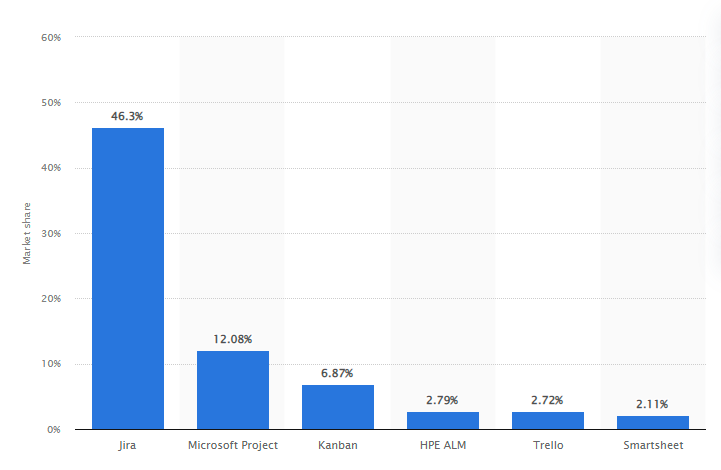
\includegraphics[width=0.95\textwidth]{marketshare.png}
    \caption{Marktanteil von Projektmanagement Software, Stand Januar 2020\cite{statista2020}}
	\label{fig:marketshare}
\end{figure}

\section{Das Weekly Standup}

Das wöchentliche beziehungsweise zweiwöchige Meeting dient dazu alle in der Projektgruppe auf dem laufenden zu halten, d.h. jedes Mitglied im Team dokumentiert für die anderen was gemacht wurde und erfährt im Gegenzug was die anderen gemacht haben.\\
Für den oder die Dozenten ist es ebenfalls wichtig zu sehen wie die Gruppe mit dem Projekt vorankommt und ob es Probleme gibt. Um den Fortschritt zu dokumentieren muss das Meeting in Schriftform stattfinden, denn wenn zum Beispiel ein Video von dem Meeting aufgezeichnet werden würde, dann wäre es ein erheblicher Aufwand für den Dozenten nachzuvollziehen was besprochen wurde. Es gibt zwar schon Technologien bei denen die gesagten Worte automatisch in Text umgewandelt werden allerdings sind diese nicht unbedingt verlässlich und darüber hinaus hat man am Ende nicht unbedingt ein strukturiertes Dokument um es auszuwerten.\\
Da es sich um Studenten und keine Mitarbeiter eines Unternehmens handelt ist auch nicht unbedingt davon auszugehen, dass alle Mitglieder in einer Gruppe zu einem festen Zeitpunkt an einem Meeting teilnehmen können oder während das Projekt läuft mit strikten Deadlines oder Sprints arbeiten werden oder können. Daher bietet es sich an das Meeting auch asynchron abzuhalten, dass heißt jeder Teilnehmer trägt unabhängig ein was seit dem letzten Meeting gemacht wurde, wo Probleme auftreten und was als nächstes gemacht wird beziehungsweise geplant ist. 

\section{Umsetzung des Daily/Weekly bei der Konkurrenz}

Wie haben die Konkurrenten das Daily/Weekly Meeting umgesetzt was können wir daraus lernen.

\subsection{Jira}

Da Jira der Marktführer ist schauen wir uns als erstes Jira im allgemeinen und die Features, die für Dailies sind im speziellen an. Jira existiert seit 2002 und hat sich als Marktführer bei Software Unternehmen etabliert. Neben den Standardfunktionalitäten bietet Jira außerdem Erweiterungen im Atlassian Marketplace an. Dabei handelt es sich um Applikationen, die Jira erweitern. Diese können von Atlassian selbst sein oder von Drittanbietern.\\
Jira geht davon aus, dass Teams entweder in Scrum oder Kanban arbeiten und bietet für diese beiden agilen Arbeitsmethoden Boards an. Die Features darum bauen auf dieser Annahme auf daher wird die Arbeit auch in Form von Tickets organisiert. Wenn ein User sich nicht an die vorgegebenen agilen Workflows hält stehen manche Funktionen wie zum Beispiel das Burn-Down Chart nicht zur Verfügung weil dafür zum Beispiel Story Points benötigt werden. Bei Studenten ist aber nicht davon auszugehen, dass sie zum einen wissen wie Story Points vergeben werden und zum andren bei so kurzen Implementierungsphasen wie es bei Projekten in der Universität der Fall ist eine aussagekräftige Schätzung abgeben können. \\
Jedes Ticket repräsentiert ein Arbeitspaket, welches im Board durch die verschiedenen Stadien im Workflow geht. Die Tickets sind wie es die Workflows vorgeben hierarchisch organisiert, d.h. es gibt verschiedene Ticket Typen wie Epic, Story, Bug und andere Tasks.

\begin{figure}[H]
	\centering
	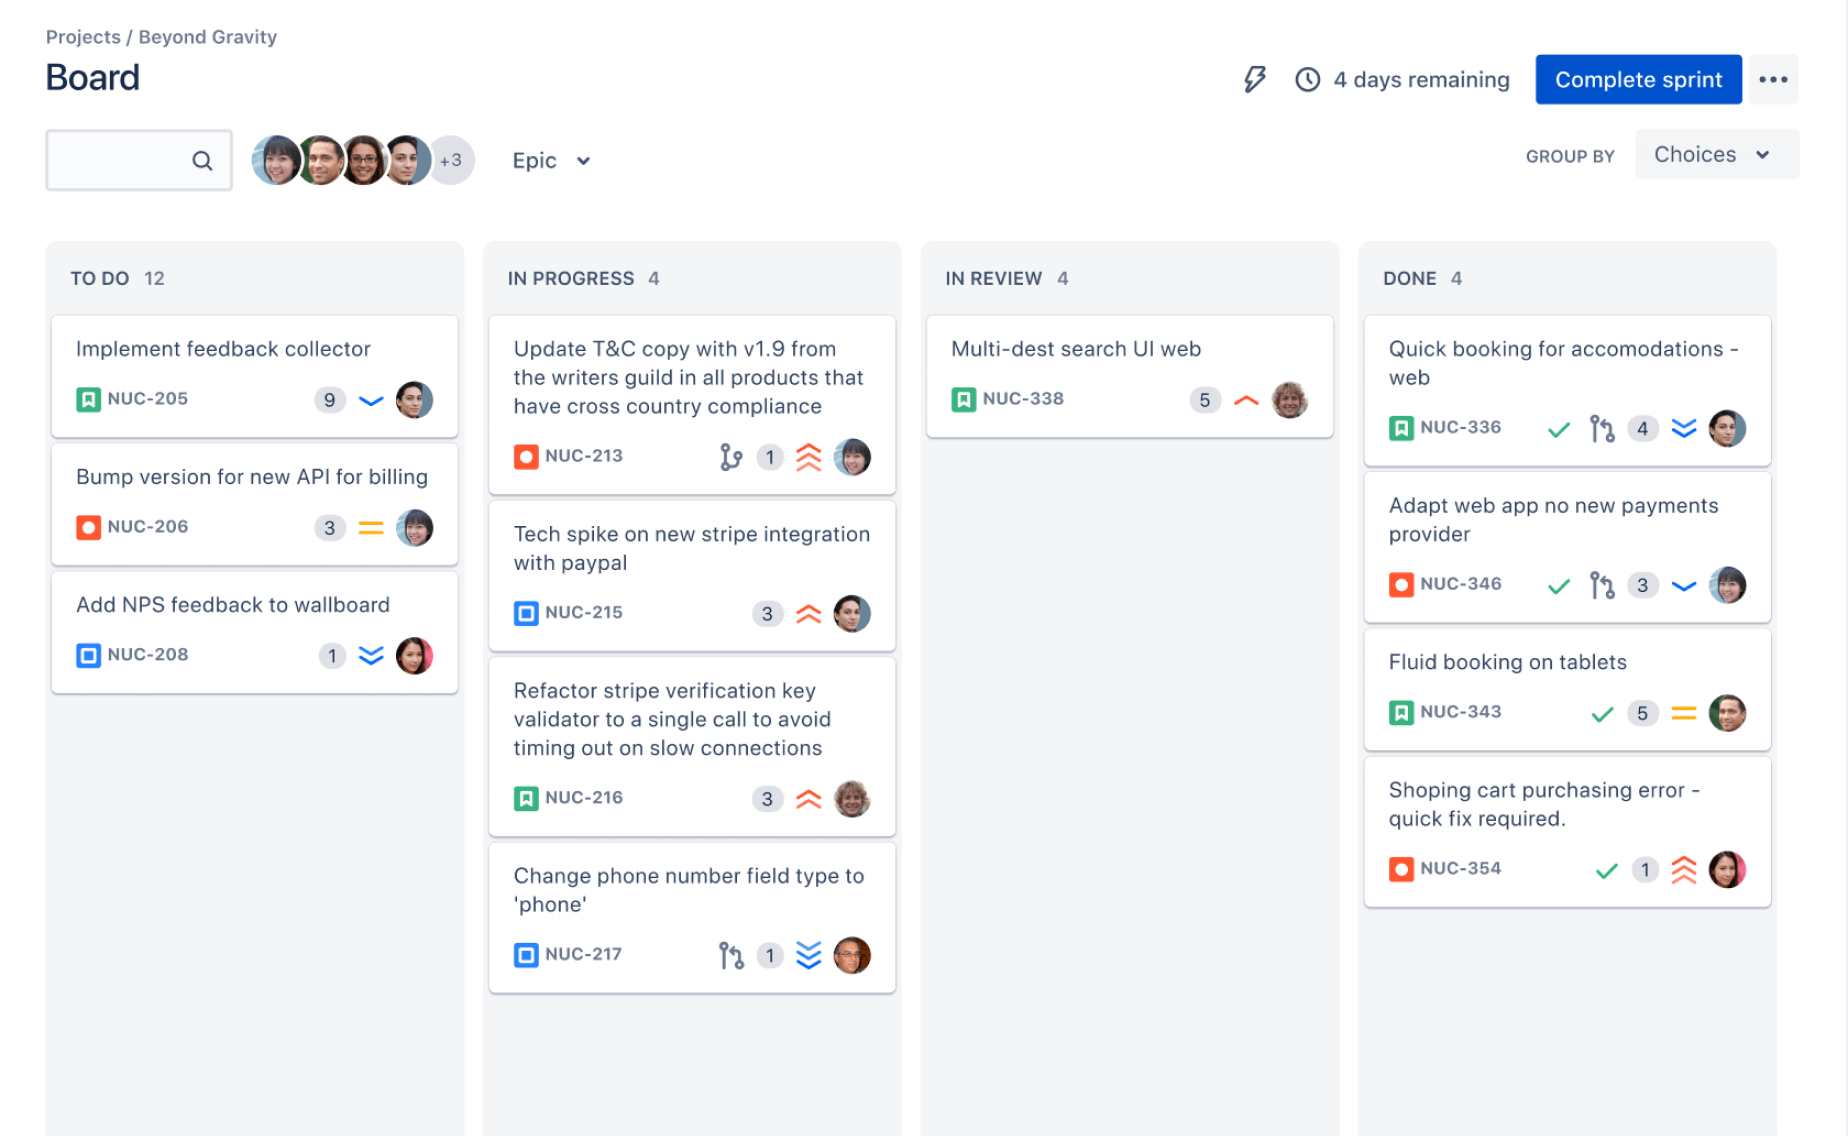
\includegraphics[width=0.95\textwidth]{jira-scrumboard.png}
    \caption{Scrum Board in Jira}
	\label{fig:scrumboardjira}
\end{figure}

Diese Ticket Typen haben eine bestimmte Hierarchie zum Beispiel kann eine Story zu einem Epic gehören und ein Bug Ticket kann ein Subtask einer Story sein. 

\begin{figure}[H]
	\centering
	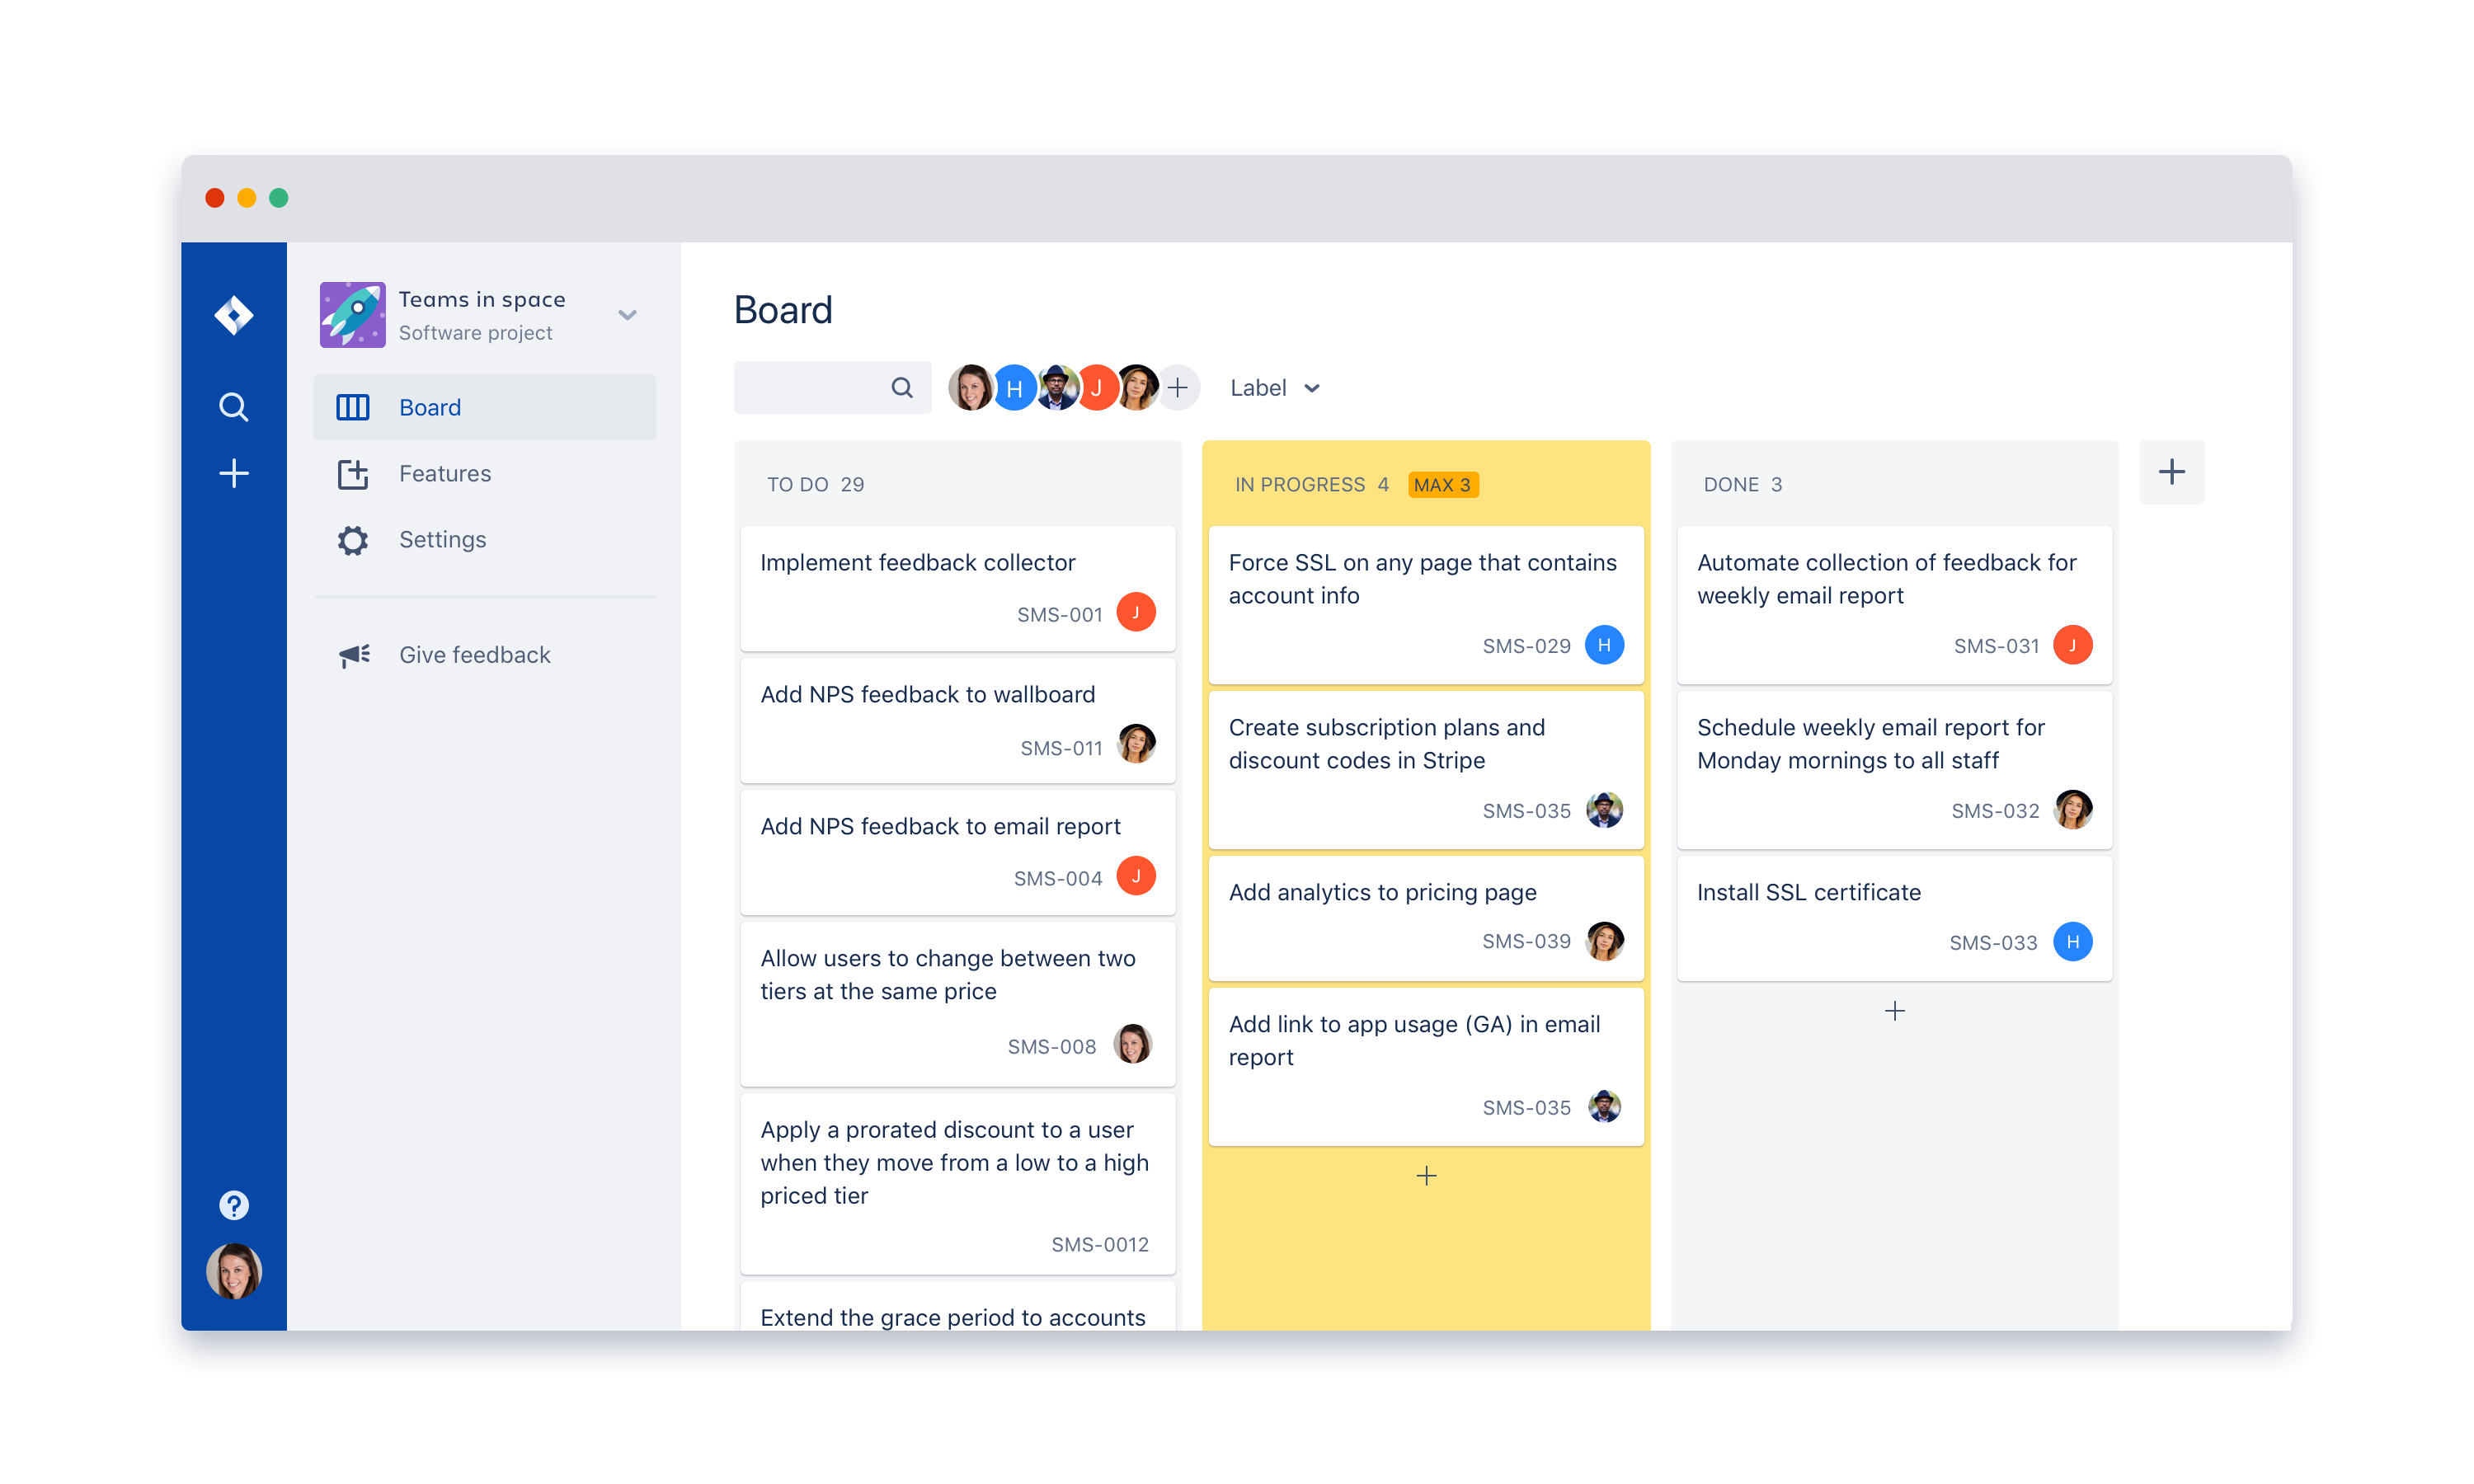
\includegraphics[width=0.95\textwidth]{jira-kanban.png}
    \caption{Kanban Board in Jira}
	\label{fig:kanbanjira}
\end{figure}

Jira ist durch die Grundfunktionalitäten und durch die Möglichkeit der Erweiterung ein sehr mächtiges Werkzeug für Studenten, die noch keine Erfahrungen mit Scrum oder Kanban haben ist es wahrscheinlich schwer den Einstieg zu finden.  Darüber hinaus ist es fraglich ob Studenten den Aufwand bei der Dokumentation innerhalb der Tickets aufwenden werden weil Projekte im universitären Kontext meist sehr kurzlebig sind.  

\begin{figure}[H]
	\centering
	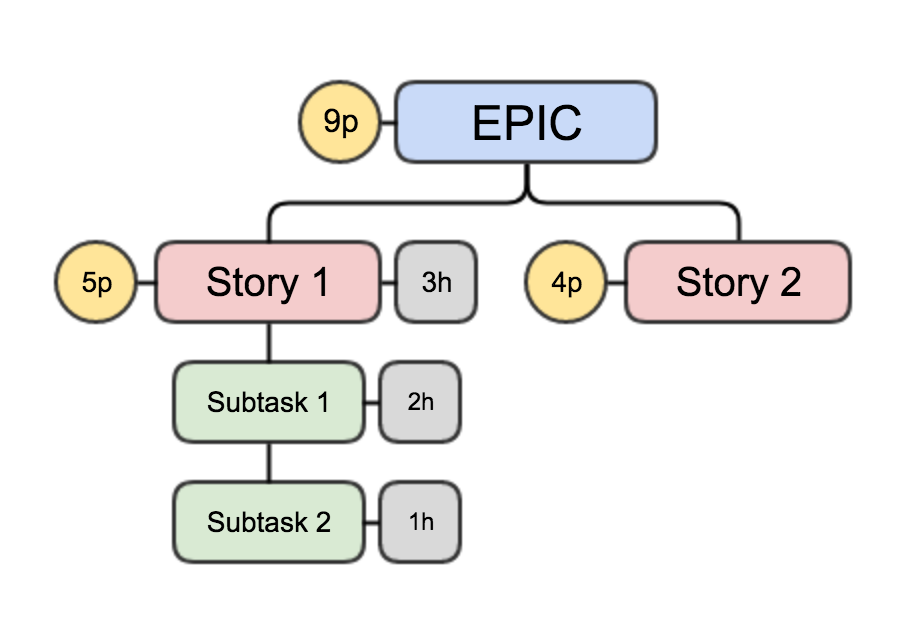
\includegraphics[width=0.95\textwidth]{jira-hierarchie.jpeg}
    \caption{Hierarchie von Tickets in Jira }
	\label{fig:hierarchyjira}
\end{figure}

Ein Dozent wäre aber genau auf die Dokumentation innerhalb der Stories beziehungsweise Tickets angewiesen um nachvollziehen zu können was genau gemacht wird oder wurde. Darüber hinaus müsste der Dozent durch die Strukturen gehen um die dokumentierte Arbeit auf den verschiedenen Ebenen sehen zu können, denn ein Kommentar zum Fortschritt kann in Form eines Kommentars in einem Eric, Story oder Sub-Task stehen. 

\begin{table}[]
    \begin{tabular}{ll}
    Vorteil         & Nachteil                                    \\
    Sehr mächtig    & Hoher Konfigurationsaufwand                 \\
    Durch Plugins erweiterbar   & Setzt Wissen über Kanban oder Scrum vorraus \\
    Workflows innerhalb eines Projekts\\
    können angepasst werden     &                                            
    \end{tabular}
\end{table}

\subsection{Microsoft Project}

Das Erscheinungsjahr von Microsoft Project ist 1984, dieses Produkt ist also schon mehrere Dekaden auf dem Markt.\\
In Microsoft Project wird davon ausgegangen, dass Projekte ein Anfangs und Enddatum haben. Darüber hinaus werden für Tass und Subtasks nicht wie bei Jira Storypunkte vergeben sondern Tage, d.h. eine Aufgabe soll dann zum Beispiel 2 Tage dauern. Microsoft Project bietet drei Ansichten für ein Projekt. \\
Die Ansichten sind
\begin{itemize}
\item Raster  
\item Board  
\item Zeitachse
\end{itemize}
In der Rasteransicht sind alle Aufgaben und deren Unteraufgaben in einer Liste angeordnet. Die Aufgaben und Unteraufgaben können erstellt, sortiert und zugewiesen werden.  

\begin{figure}[H]
	\centering
	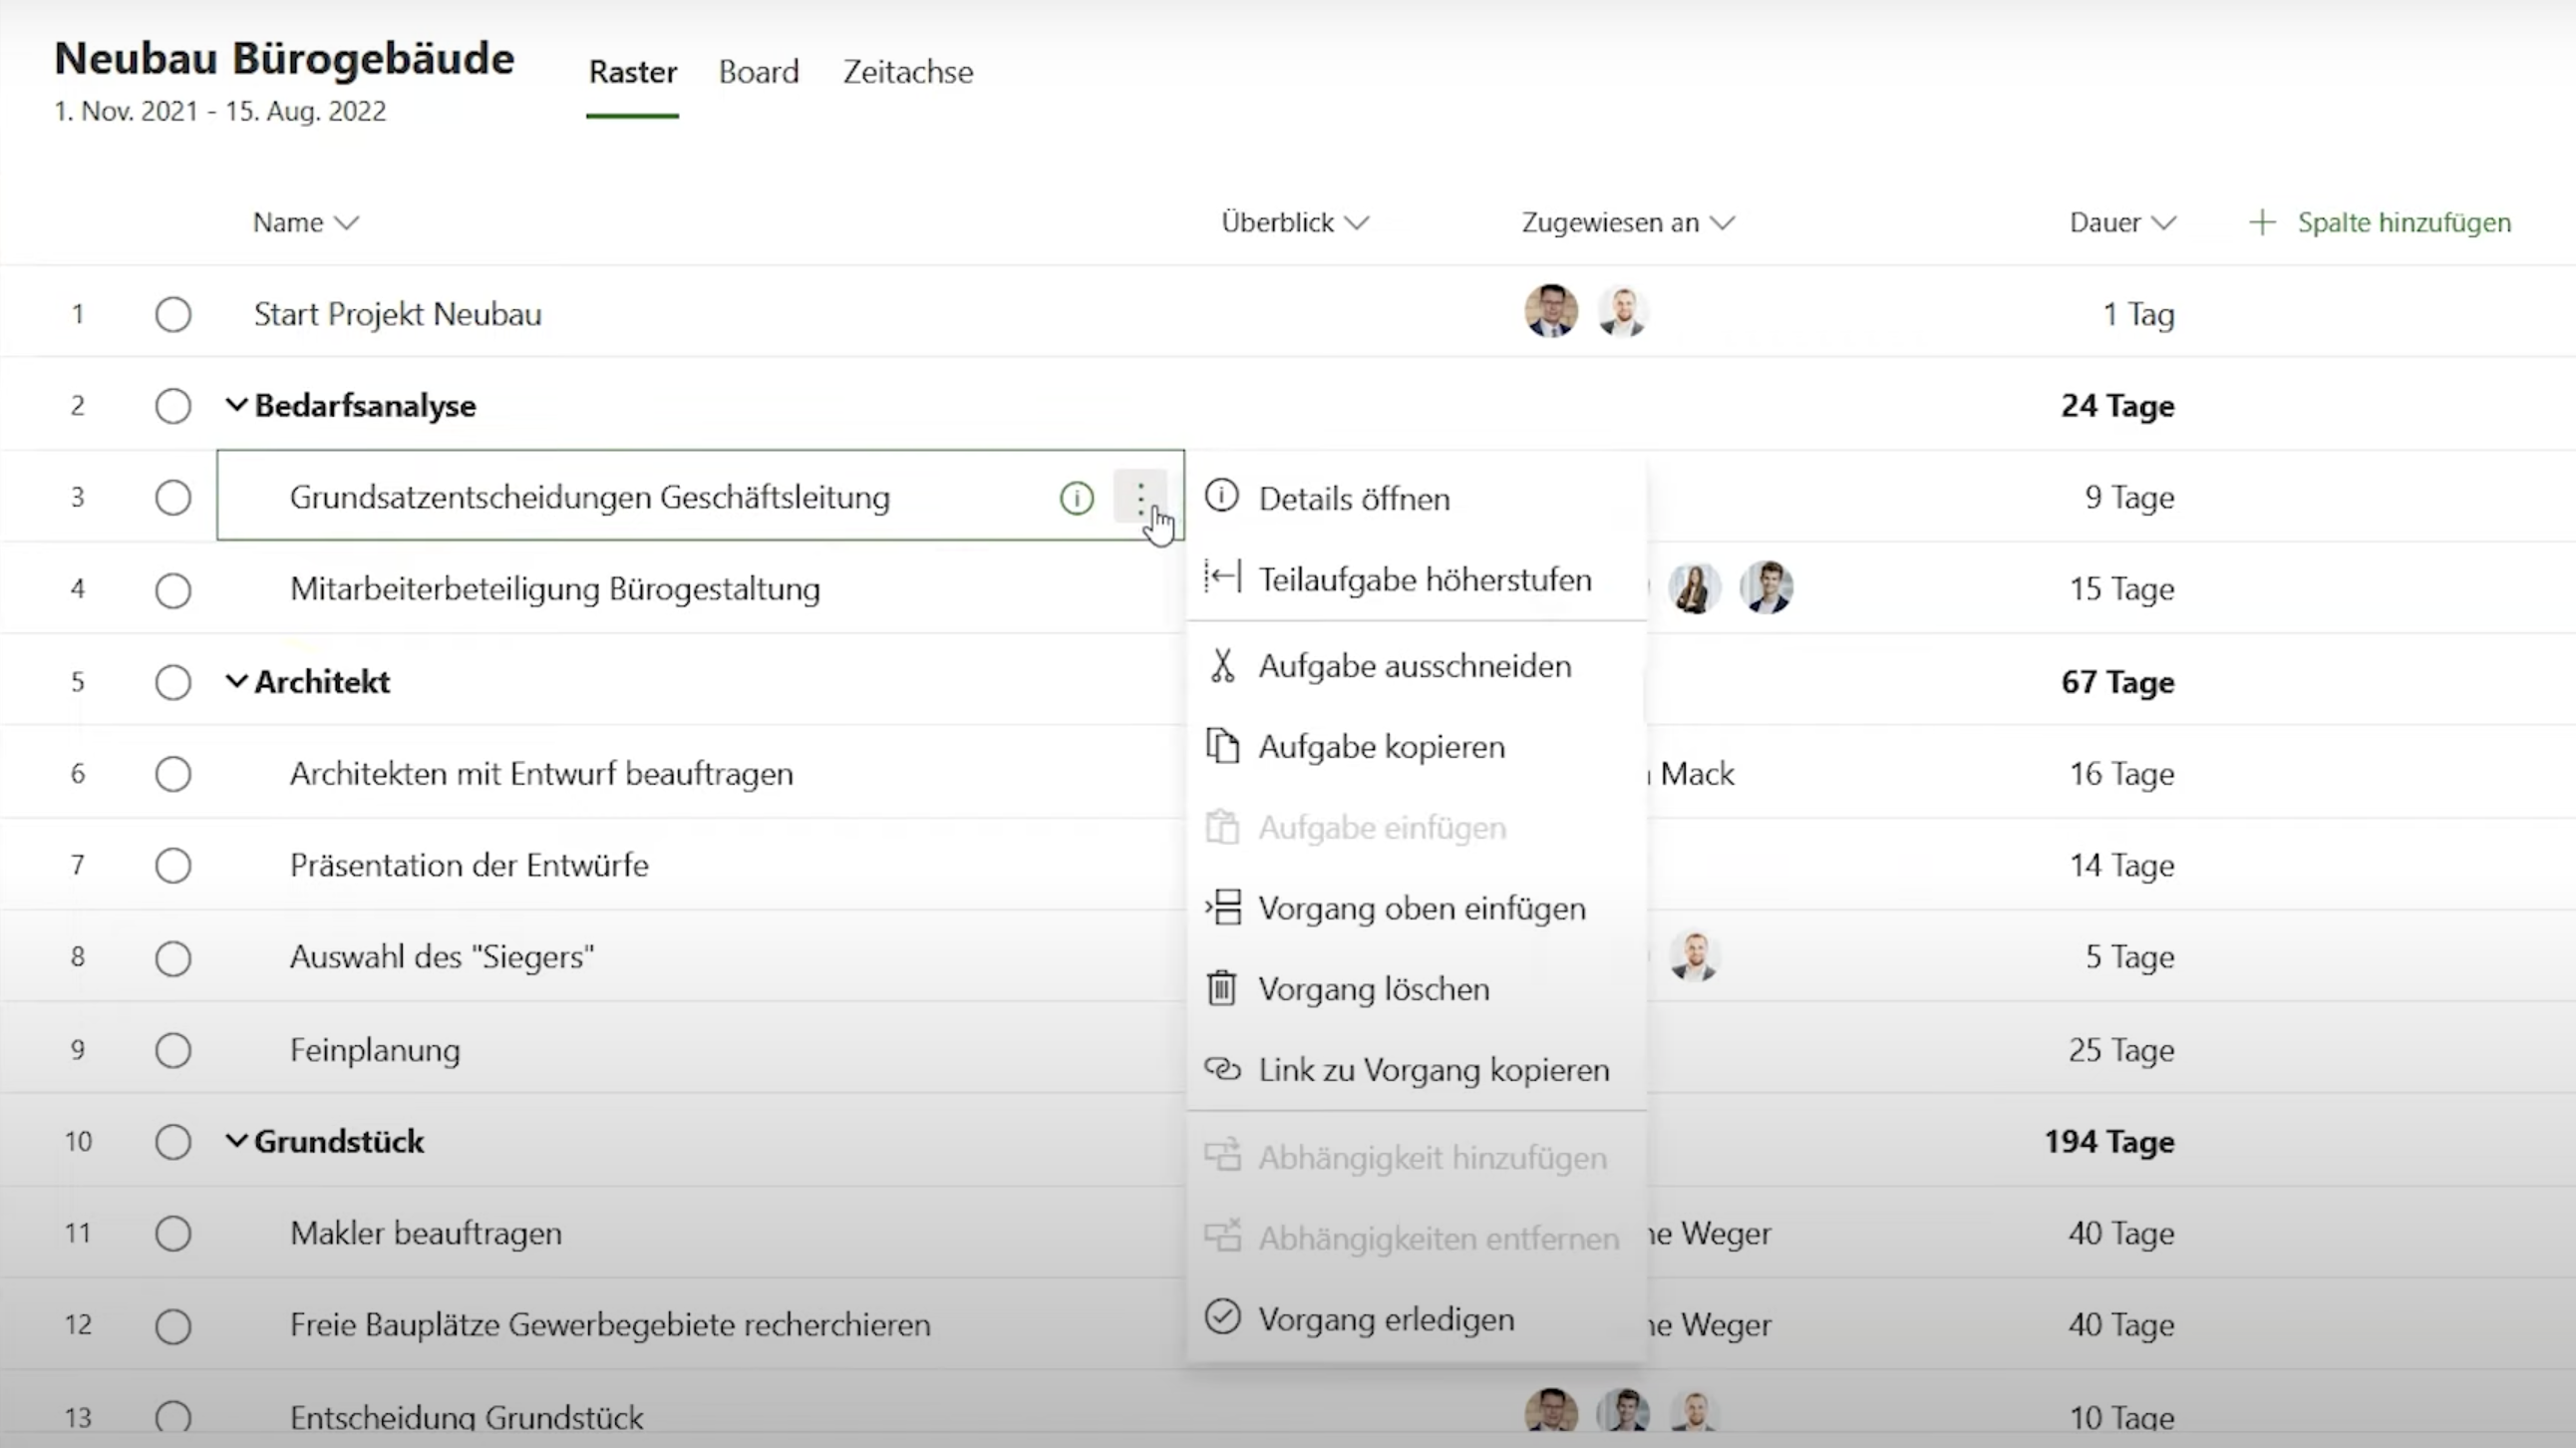
\includegraphics[width=0.95\textwidth]{ms-project-raster.png}
    \caption{Rasteransicht eines Projektes in Microsoft Project}
	\label{fig:rastermsproject}
\end{figure}

Die Aufgaben in Microsoft Project haben als default nur ein Feld für Notizen, d.h. eine Story würde hier nur aus der Headline und einer Notiz bestehen. Der Fokus scheint nicht wie bei Jira auf Softwareprojekte gerichtet zu sein.  

\begin{figure}[H]
	\centering
	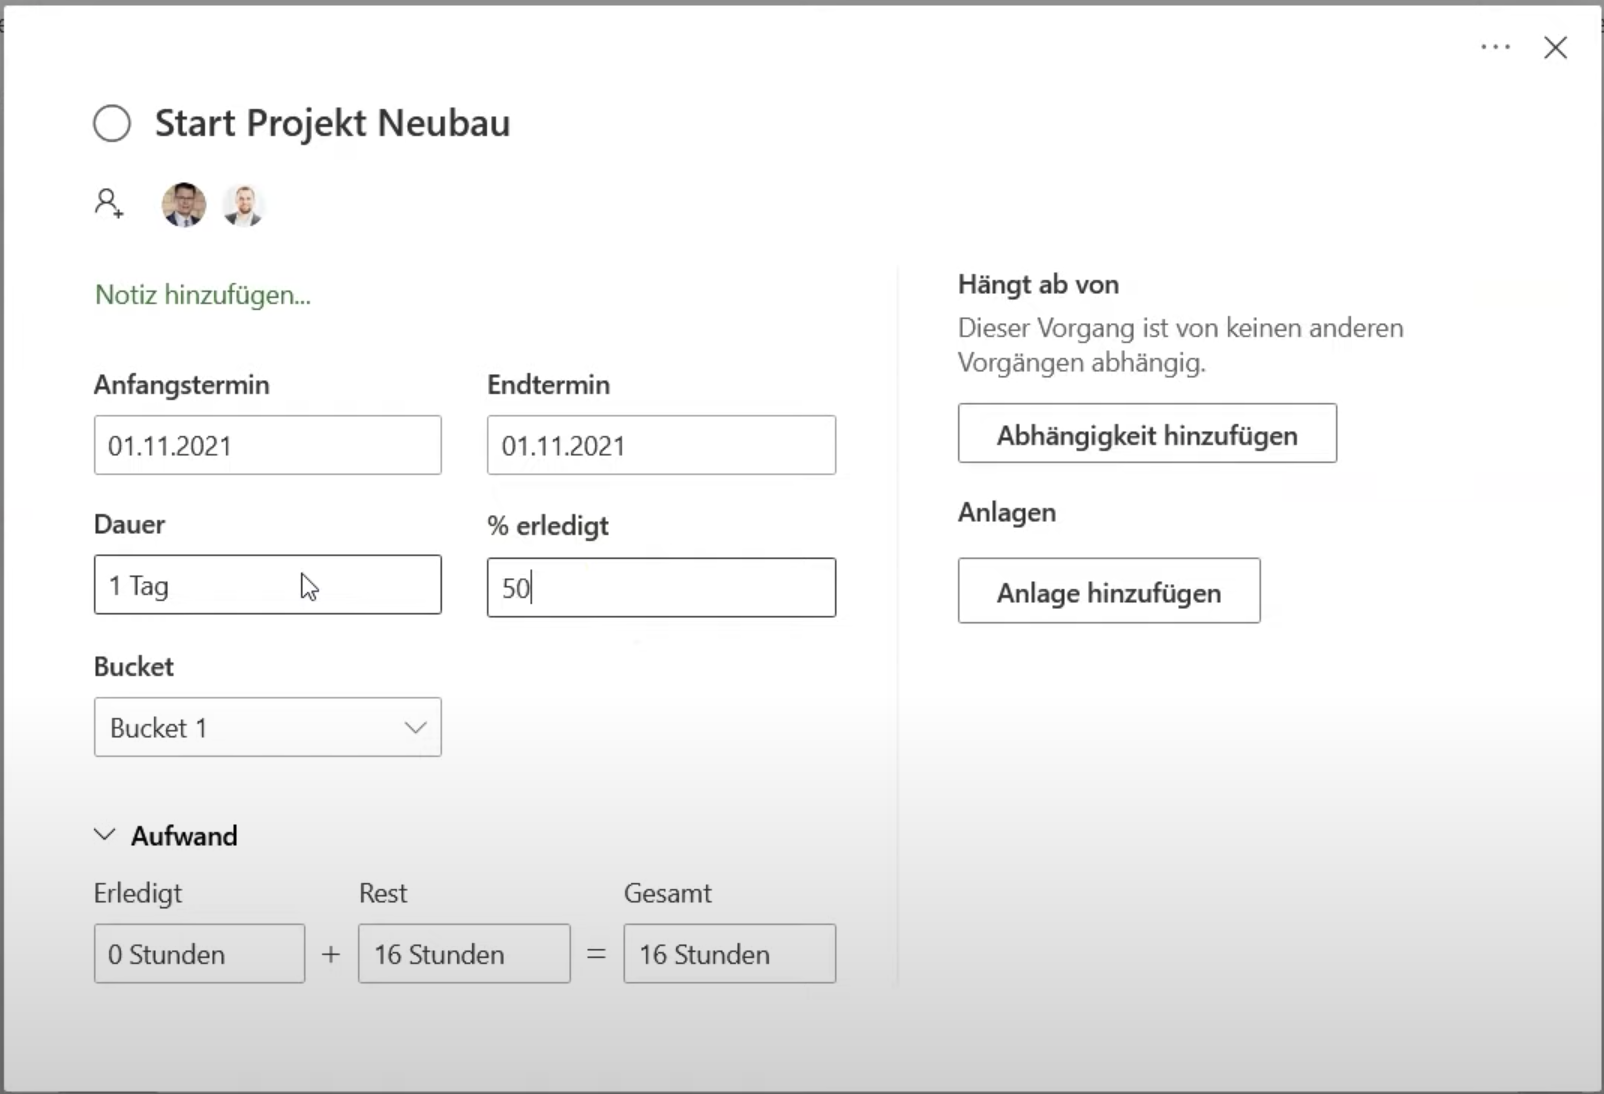
\includegraphics[width=0.95\textwidth]{ms-project-task.png}
    \caption{Eine Aufgabe in Microsoft Project}
	\label{fig:taskmsproject}
\end{figure}

In der Board Ansicht gibt es drei Spalten für die Aufgaben des Projekts\\
\begin{itemize}
    \item Nicht begonnen 
    \item In Arbeit  
    \item Erledigt
\end{itemize}
In dieser Ansicht sind die Aufgaben als Karten dargestellt. Jede Karte hat das Thema, den Bucket, das Fälligkeitsdatum, den Prozentualen Fortschritt und die Icons mit Bildern der Personen, die diese Aufgabe zugewiesen haben. Das Kanban Board kann aber konfiguriert werden um zum Beispiel mehr Spalten oder andere Informationen in den Karten anzuzeigen.\\

\begin{figure}[H]
	\centering
	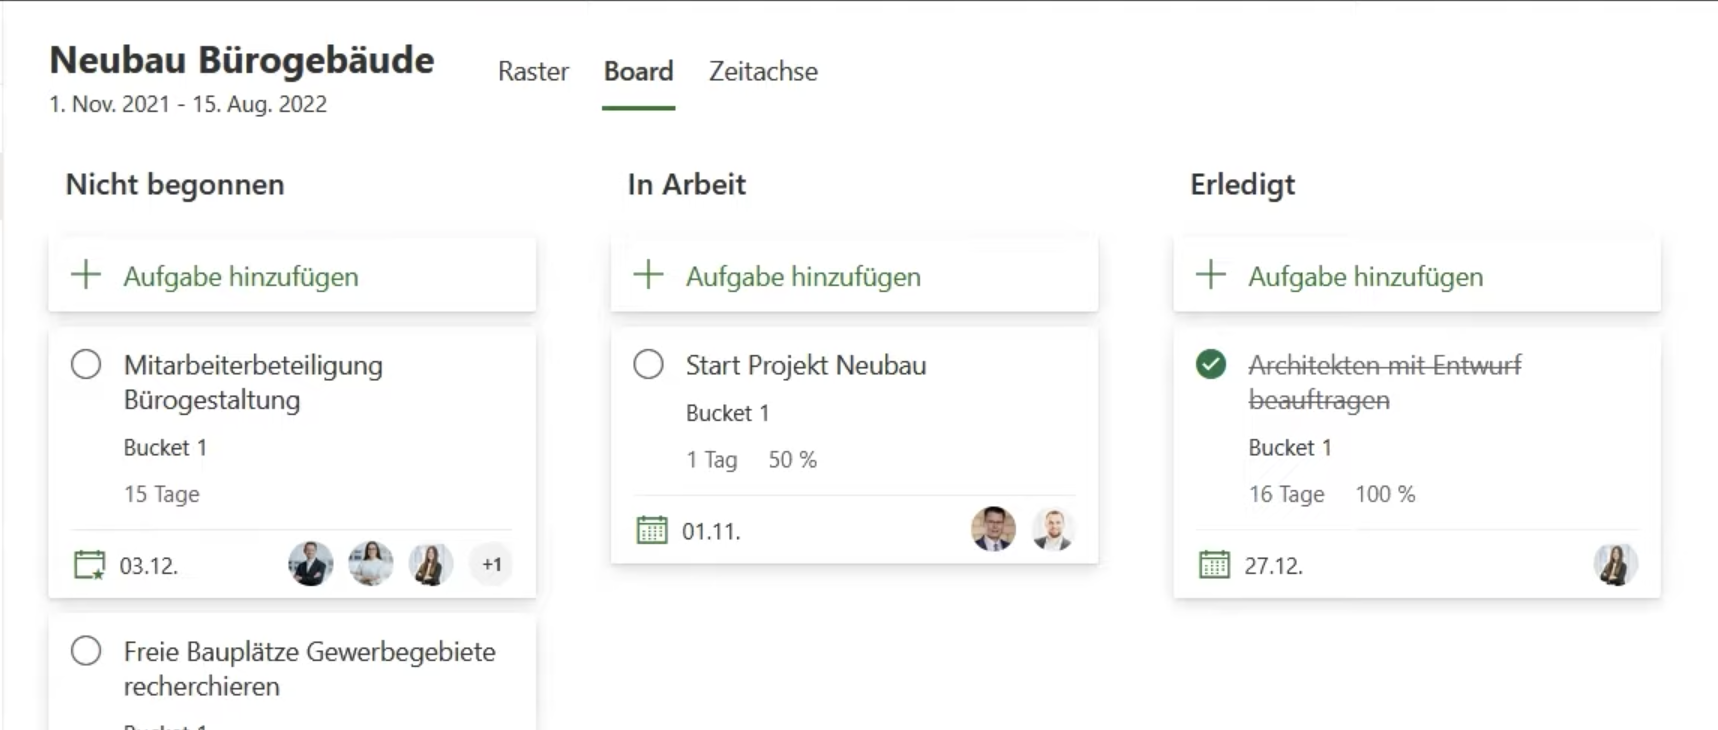
\includegraphics[width=0.95\textwidth]{ms-project-kanban.png}
    \caption{Kanban Board in Microsoft Project}
	\label{fig:kanbanmsproject}
\end{figure}

In der Zeitachsen Ansicht wird auf der linken Seite die Liste mit den Aufgaben angezeigt und auf der rechten Seite wird ein Graph aus den Aufgaben erstellt. Dabei hat jede Aufgabe eine Zeile und eine Länge auf der Zeitachse.\\
Abhängigkeiten werden durch Pfeile dargestellt. Ein Pfeil geht von links nach rechts, d.h. die Abhängigkeiten werden im zeitlichen Ablauf dargestellt. Die Aufgaben können in dieser Ansicht auf der Zeitachse verlängert oder verkürzt werden.\\

\begin{figure}[H]
	\centering
	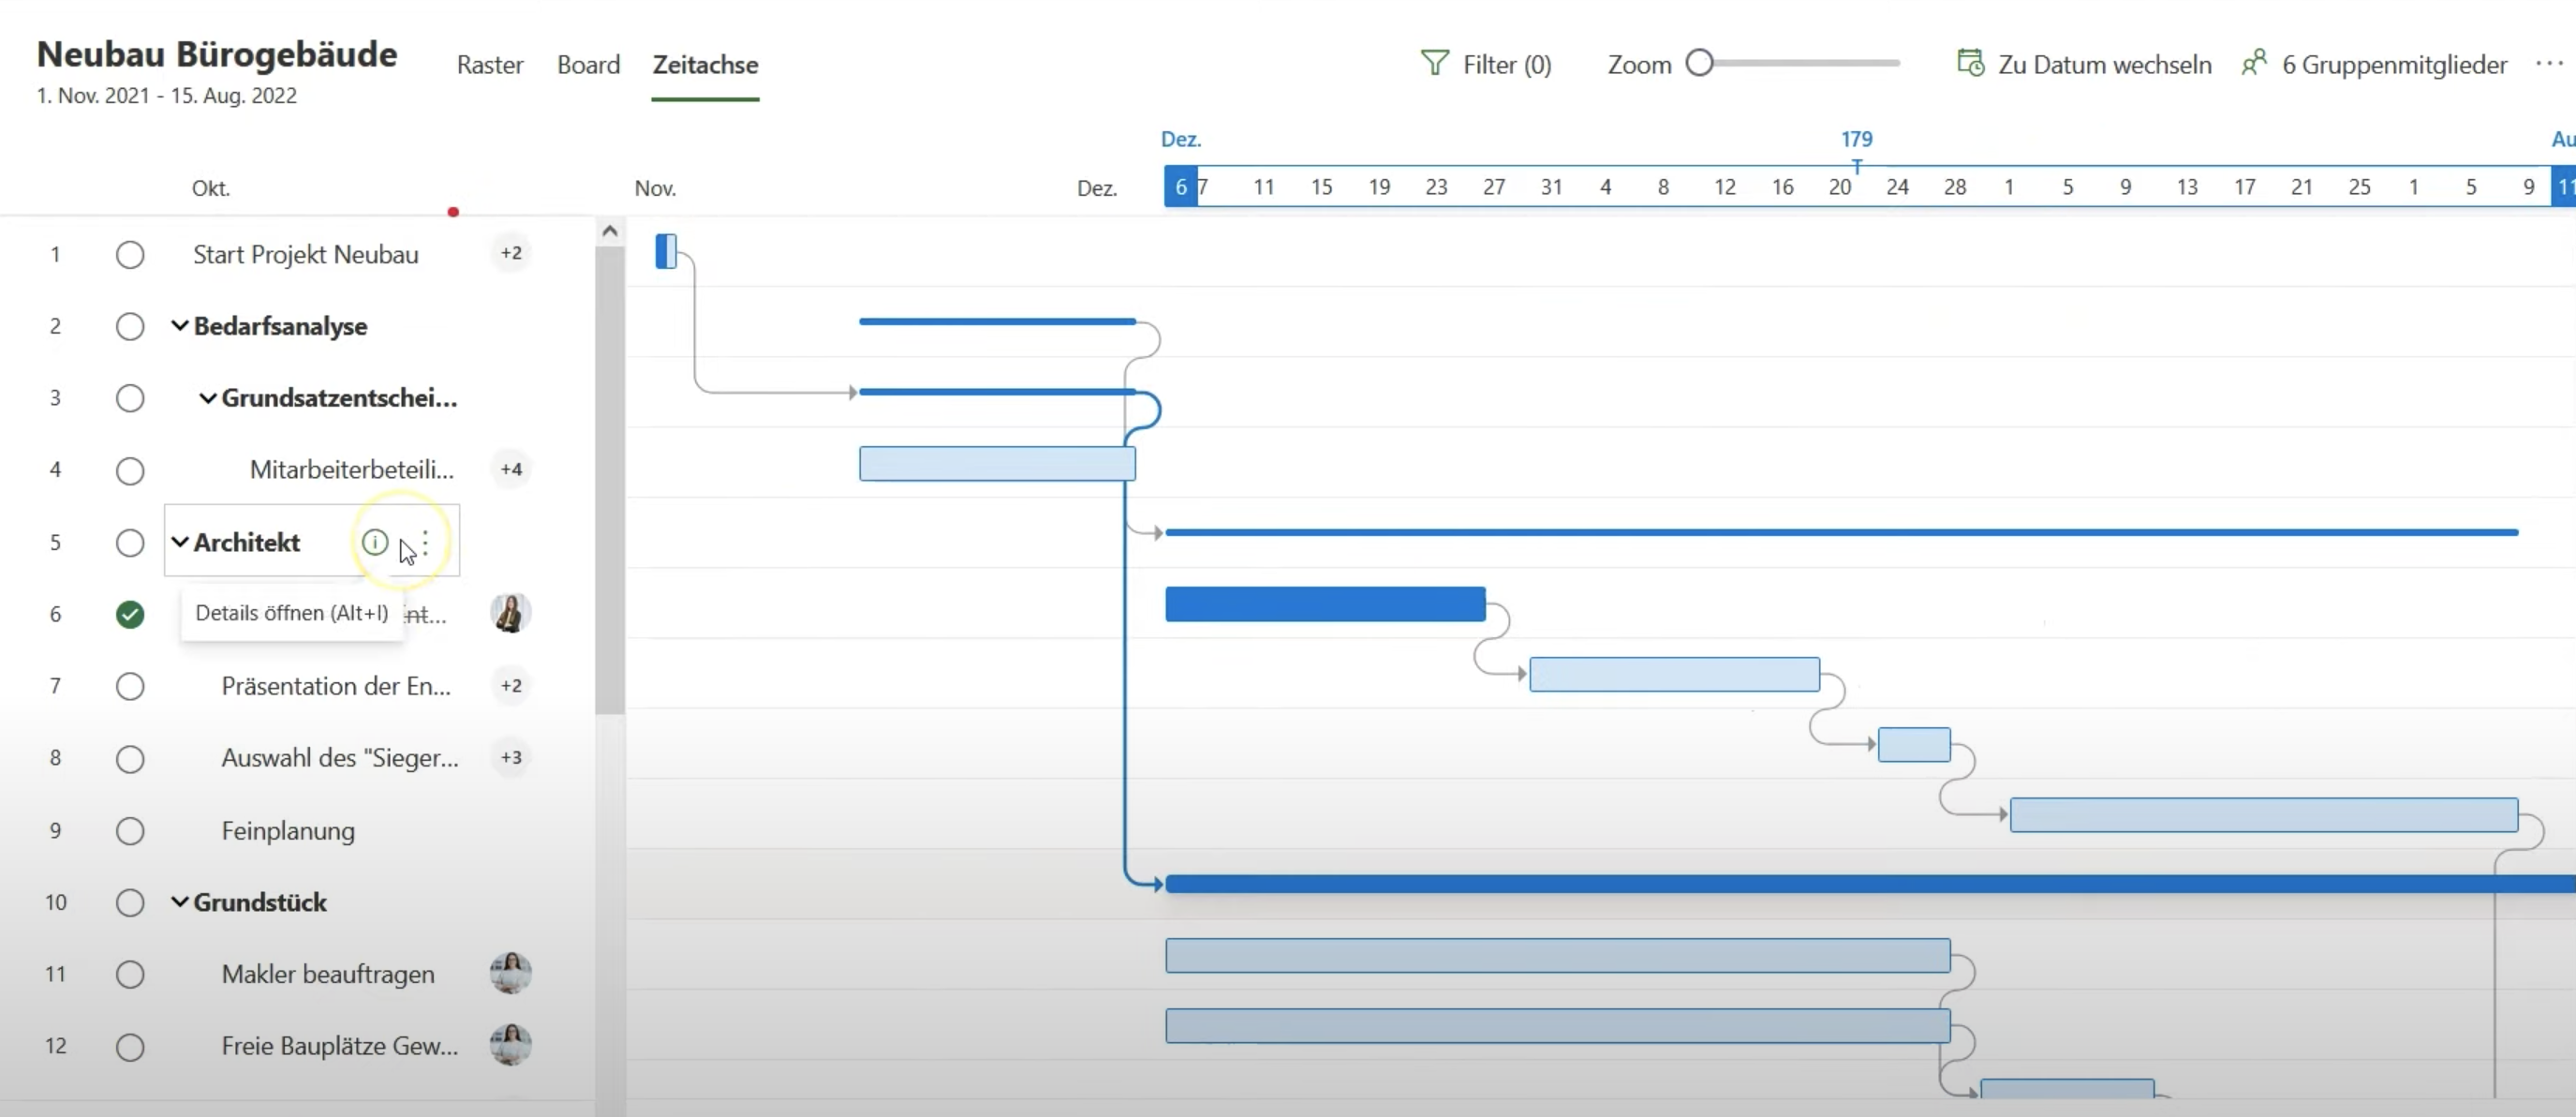
\includegraphics[width=0.95\textwidth]{ms-project-timeline.png}
    \caption{Zeitachse in Microsoft Project}
	\label{fig:timelinemsproject}
\end{figure}

Für Projektleiter oder Abteilungsleiter gibt es auch eine Ansicht für Roadmaps in denen man auf einer Zeitachse mehrere Projekte zu sehen. Es können auch Aufgaben auf dieser Ebene hinzugefügt werden. Diese Ansicht wäre für Dozenten interessant. Zusammenfassend lässt sich sagen, dass Microsoft von den Features interessant für Studentenprojekte ist allerdings braucht jeder Student dann eine Lizenz für diese Software, da normale Office 365 Nutzer nur Lesezugriff haben. Für Softwareprojekte stellt sich auch noch die Frage des Konfigurationsaufwands um zum Beispiel eine Story korrekt darzustellen in der dann mehr als eine Notiz drin ist wie zum Beispiel Designs oder Testfälle.  Eine Funktion für ein Daily oder Weekly Meeting gibt es als Default nicht, d.h. es müsste alles manuell in den einzelnen Aufgaben dokumentiert werden, was auf der Seite der Dozenten einen erheblichen Mehraufwand darstellt.  

\subsection{Asana Kanban}

Asana wurde 2008 gegründet und ist seit 2012 kommerziell davor war es ostenlos. In Asana gibt es wie bei Microsoft Project verschiedenen Ansichten. Beim Erstellen des Projekts wird eine Default Ansicht ausgewählt dabei kann man aus 4 verschiednen Optionen wählen:
\begin{itemize}
    \item List 
    \item Board 
    \item Timeline  
    \item Calendar 
\end{itemize}

Im Kanban Board sieht man wie bei Jira oder Microsoft Project als Default 3 Spalten:
\begin{itemize}
    \item To Do
    \item In Progress
    \item Complete
\end{itemize}

Innerhalb der Tasks kann man sehen welcher Person das Task zugewiesen wurde, welche Zeitraum vorgesehen ist.

\begin{figure}[H]
	\centering
	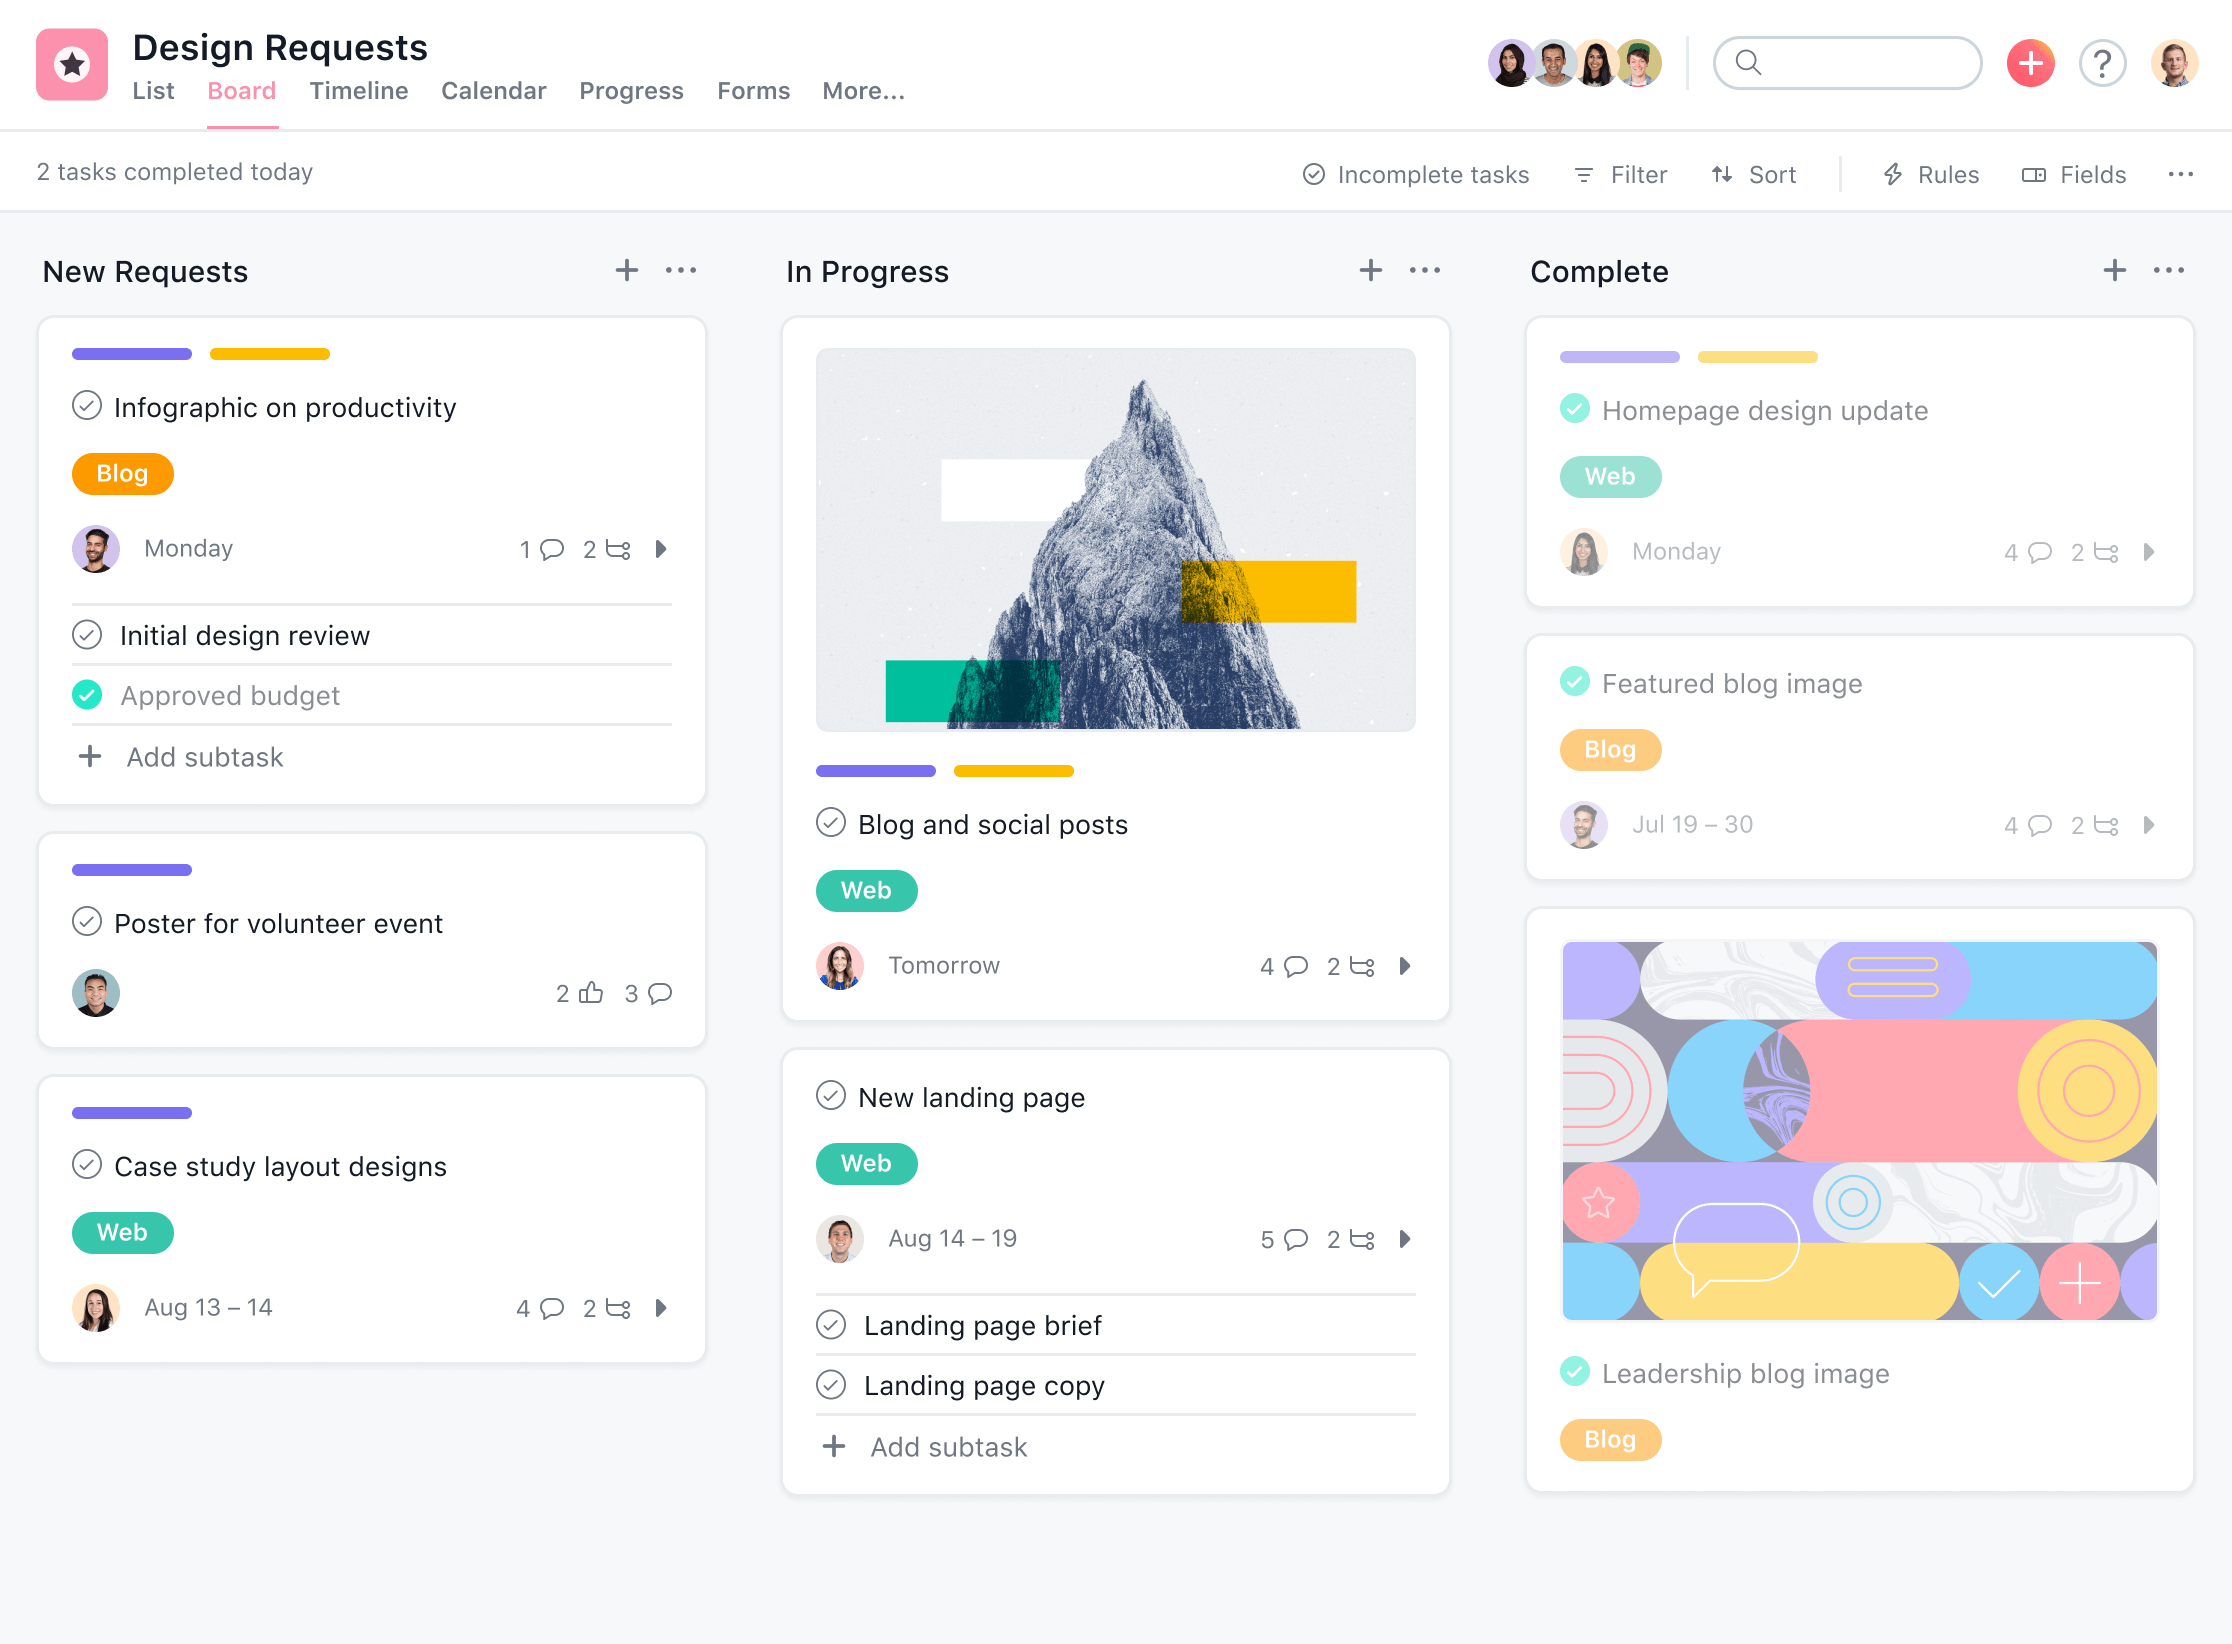
\includegraphics[width=0.95\textwidth]{asana-kanban.png}
    \caption{Kanban Board in Asana}
	\label{fig:kanbanasana}
\end{figure}


Außerdem sieht man die Subtasks und falls Bilder hinzugefügt wurden eine Vorschau des Bildes in dem Ticket. Für Meetings gibt es in Asana „Meeting Agenda Projects“. Es gibt hier zwei mögliche Ansichten List und Board. In der List Ansicht wird für jedes Punkt der Agenda ein Task hinzugefügt. Es können dann als nächstes die Teilnehmer zu dem Meeting Projekt hinzugefügt werden. Neue Tasks können dann während des Meetings hinzugefügt werden.

\begin{figure}[H]
	\centering
	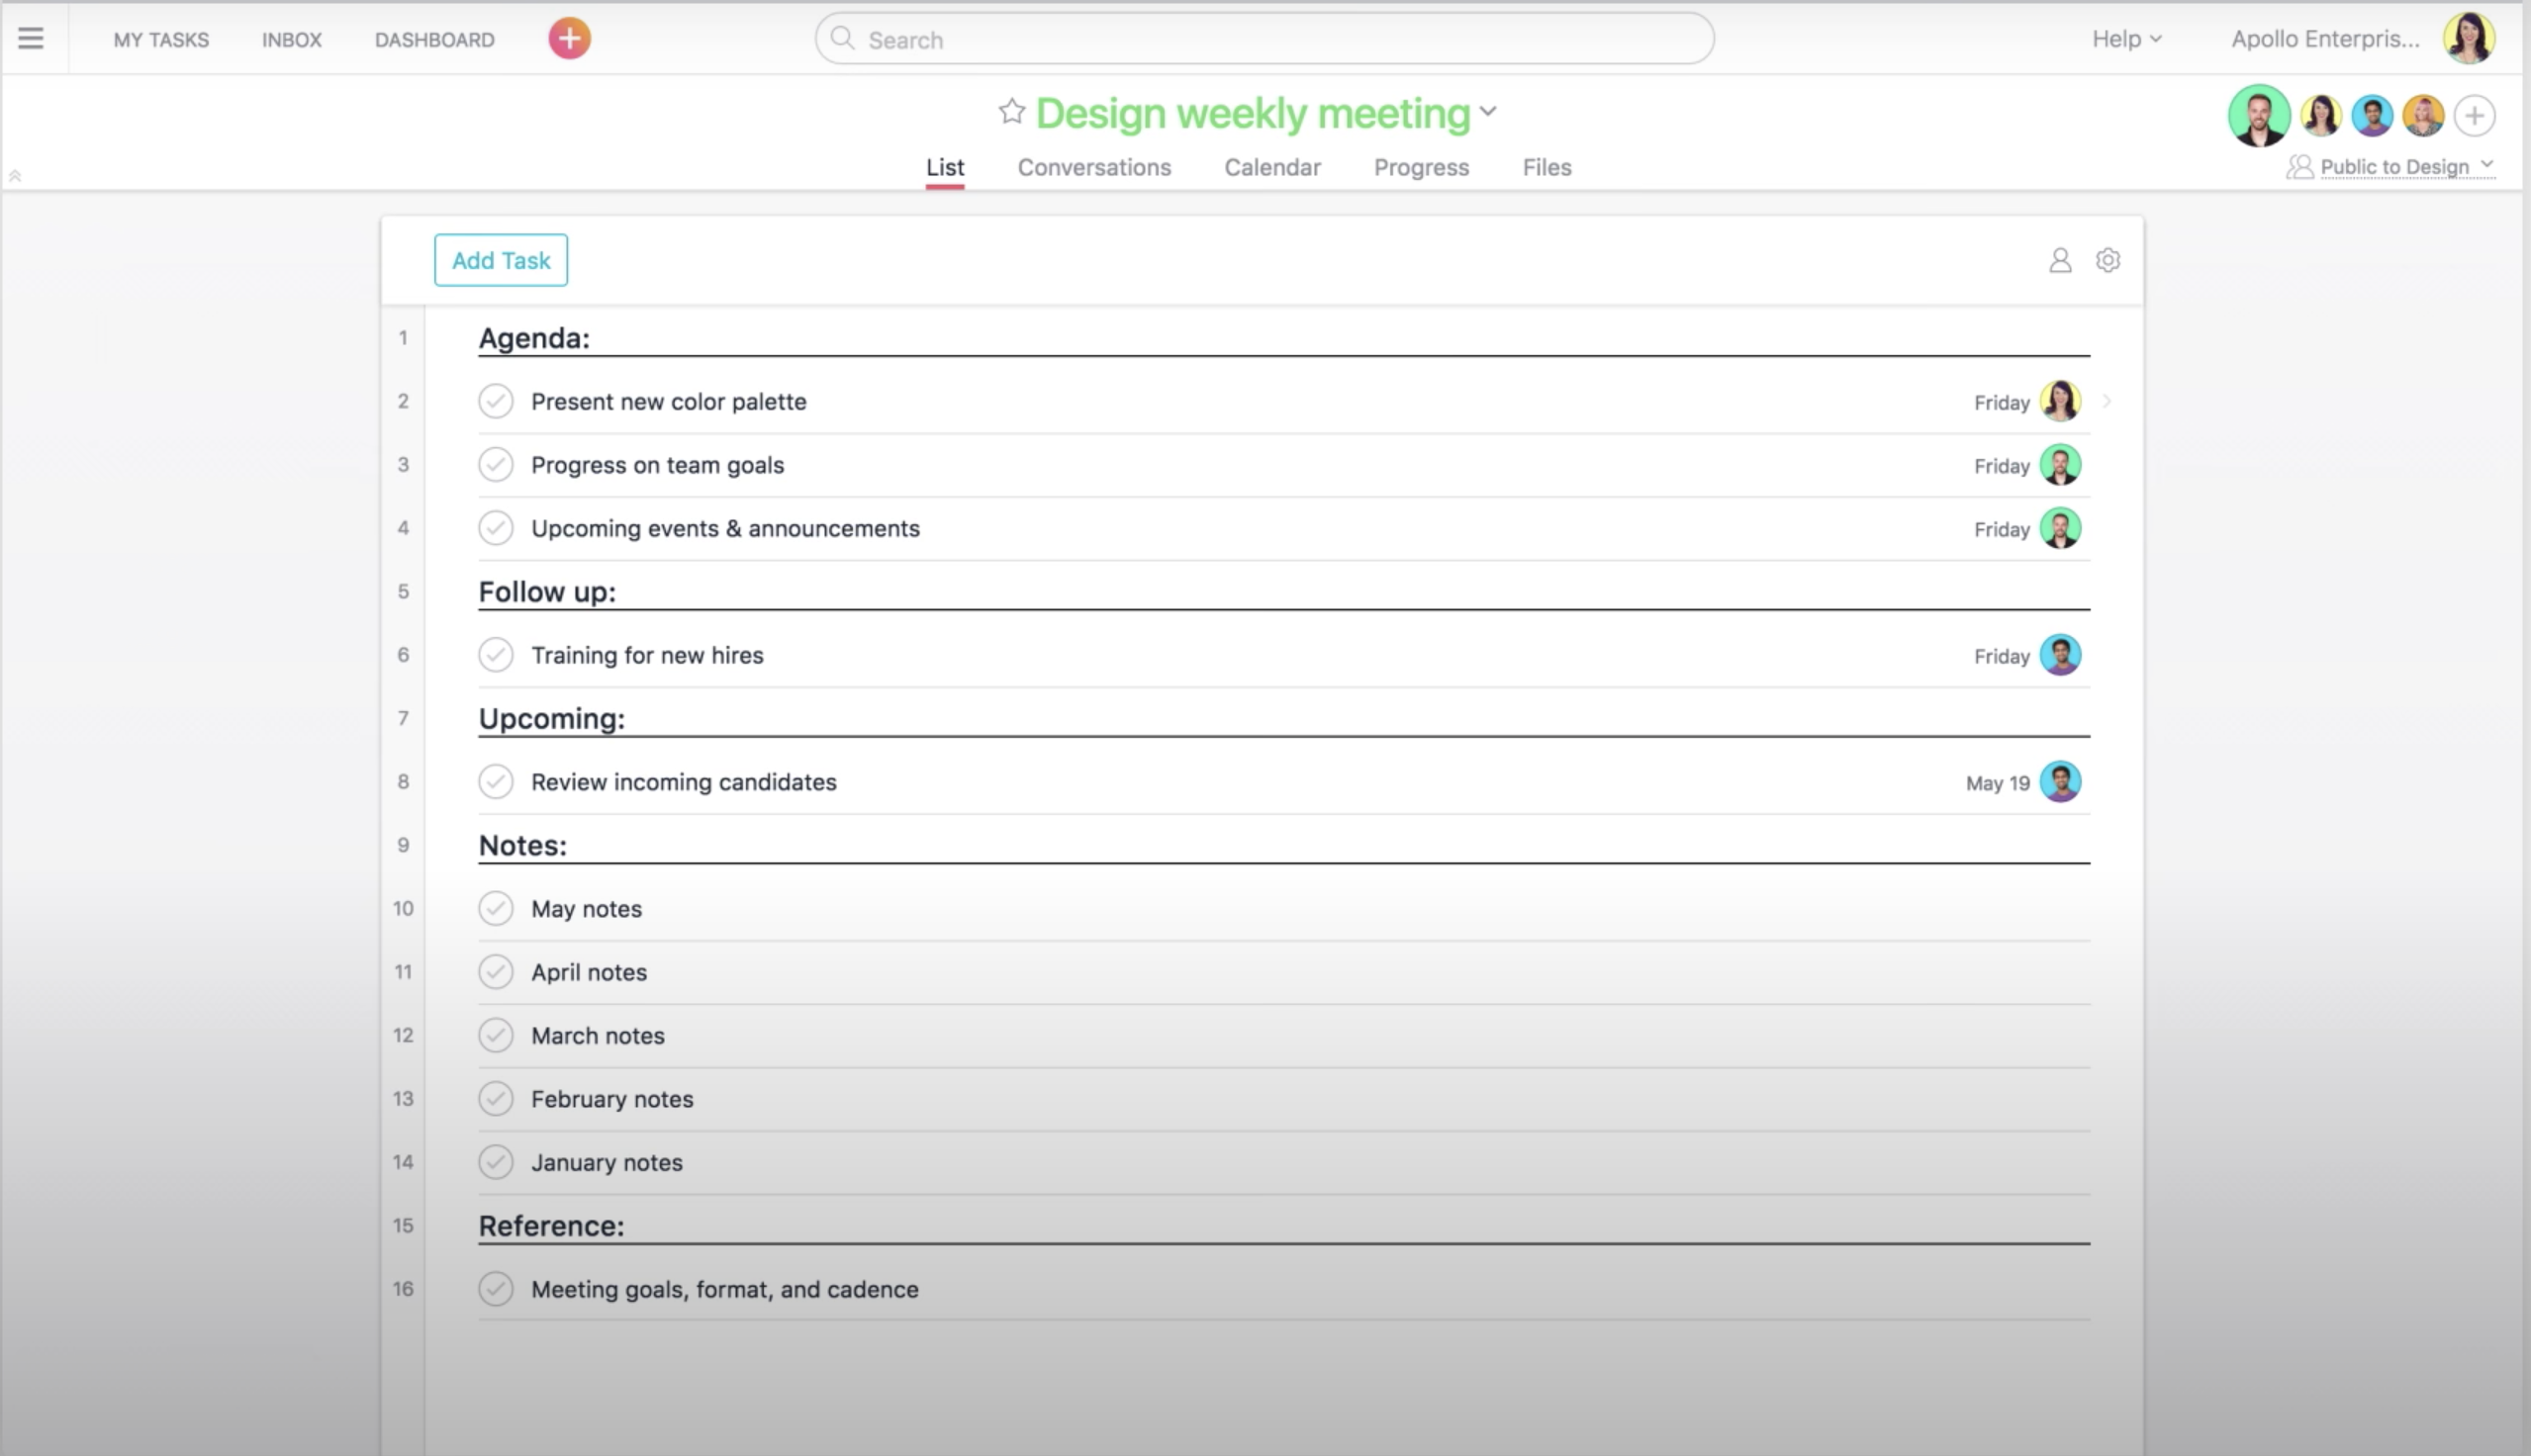
\includegraphics[width=0.95\textwidth]{asana-weekly.png}
    \caption{Weekly in Asana}
	\label{fig:weeklyasana}
\end{figure}

Die Tasks in dem Meeting Projekt können per Drag \& Drop in der Agenda bewegt werden. Fertige Tasks können abgehakt werden. Für die Tasks kann jeweils ein Fälligkeitsdatum gesetzt werden.\\
Asana ist von den vorgestellten Lösungen am interessantesten allerdings bietet es nicht die Möglichkeit automatisch ein wiederkehrendes Meeting zu konfigurieren so wie es Studenten und Dozenten in einem universitären Projekt brauchen zumindest nicht out of the box.

\section{Ergebnis}

Welche Stärken und Schwächen haben die Konkurrenzprodukte?\\

Zunächst lässt sich feststellen, dass keines der analysierten Konkurrenzprodukte ein ähnliches Feature hat. Der Grund dafür wird in dem Fokus auf Unternehmen liegen. Es gibt Features für Reports aber auch hier haben sie ein anderes Ziel als wir es im universitären Kontext brauchen, denn in einem Unternehmen werden Mitarbeiter zwar bewertet aber nicht in der gleichen Weise wie in einer Lehranstalt.\\
Jira richtet sich an agil arbeitenden Firmen mit einem Fokus auf Scrum und Kanban. Die Projekte haben hier normalerweise keine feste Deadline. Die Schätzungen durch das Team sind essentiell in Jira, denn ohne sie funktionieren eine Reihe von Reports nicht. Ob Studenten ohne Vorwissen in der Lage sind Schätzungen abzugeben ist fraglich und es würde sich dann auch die Frage 
nach Plannings und einem Scrum Master stellen.\\
Microsoft Project richtet sich an Unternehmen mit Projekten, die nach dem Wasserfall Prinzip abgearbeitet werden, deswegen haben Tasks dort auch per default ein Fälligkeitsdatum. Im universitären Kontext trifft das schon eher auf Projekte zu, wenn sie zum Beispiel innerhalb eines laufenden Semesters bearbeitet werden müssen.  Allerdings hat man hier das Problem mit den Lizenzen, da jedes Teammitglied eine aktive Lizenz braucht um mehr zu tun als zu lesen. Falls es von der jeweiligen Universität eine Partnerschaft gibt könnte es funktionieren Microsoft Projects einzusetzen allerdings bietet es kein Feature um Weekly Meetings so zu dokumentieren, dass es schnell und einfach durch den Dozenten erfasst werden kann.\\
Asana ist eine Mischung aus Jira und Microsoft Project, denn man hat hier auch die verschieden Ansichten aber einen stärkeren Fokus auf agiles Arbeiten als bei Microsoft Project. Im Gegensatz zu den andren beiden gibt es hier die Möglichkeit ein extra Meeting Project aufzusetzen allerdings bietet diese Projektart auch nicht was wir brauchen beziehungsweise entwickeln wollen. 

\clearpage
	\chapter{Personas}

Für die Implementierung des Moduls haben wir folgende Personas entwickelt

\section{Persona A: Charlie Blomquist}

\begin{figure}[H]
	\centering
	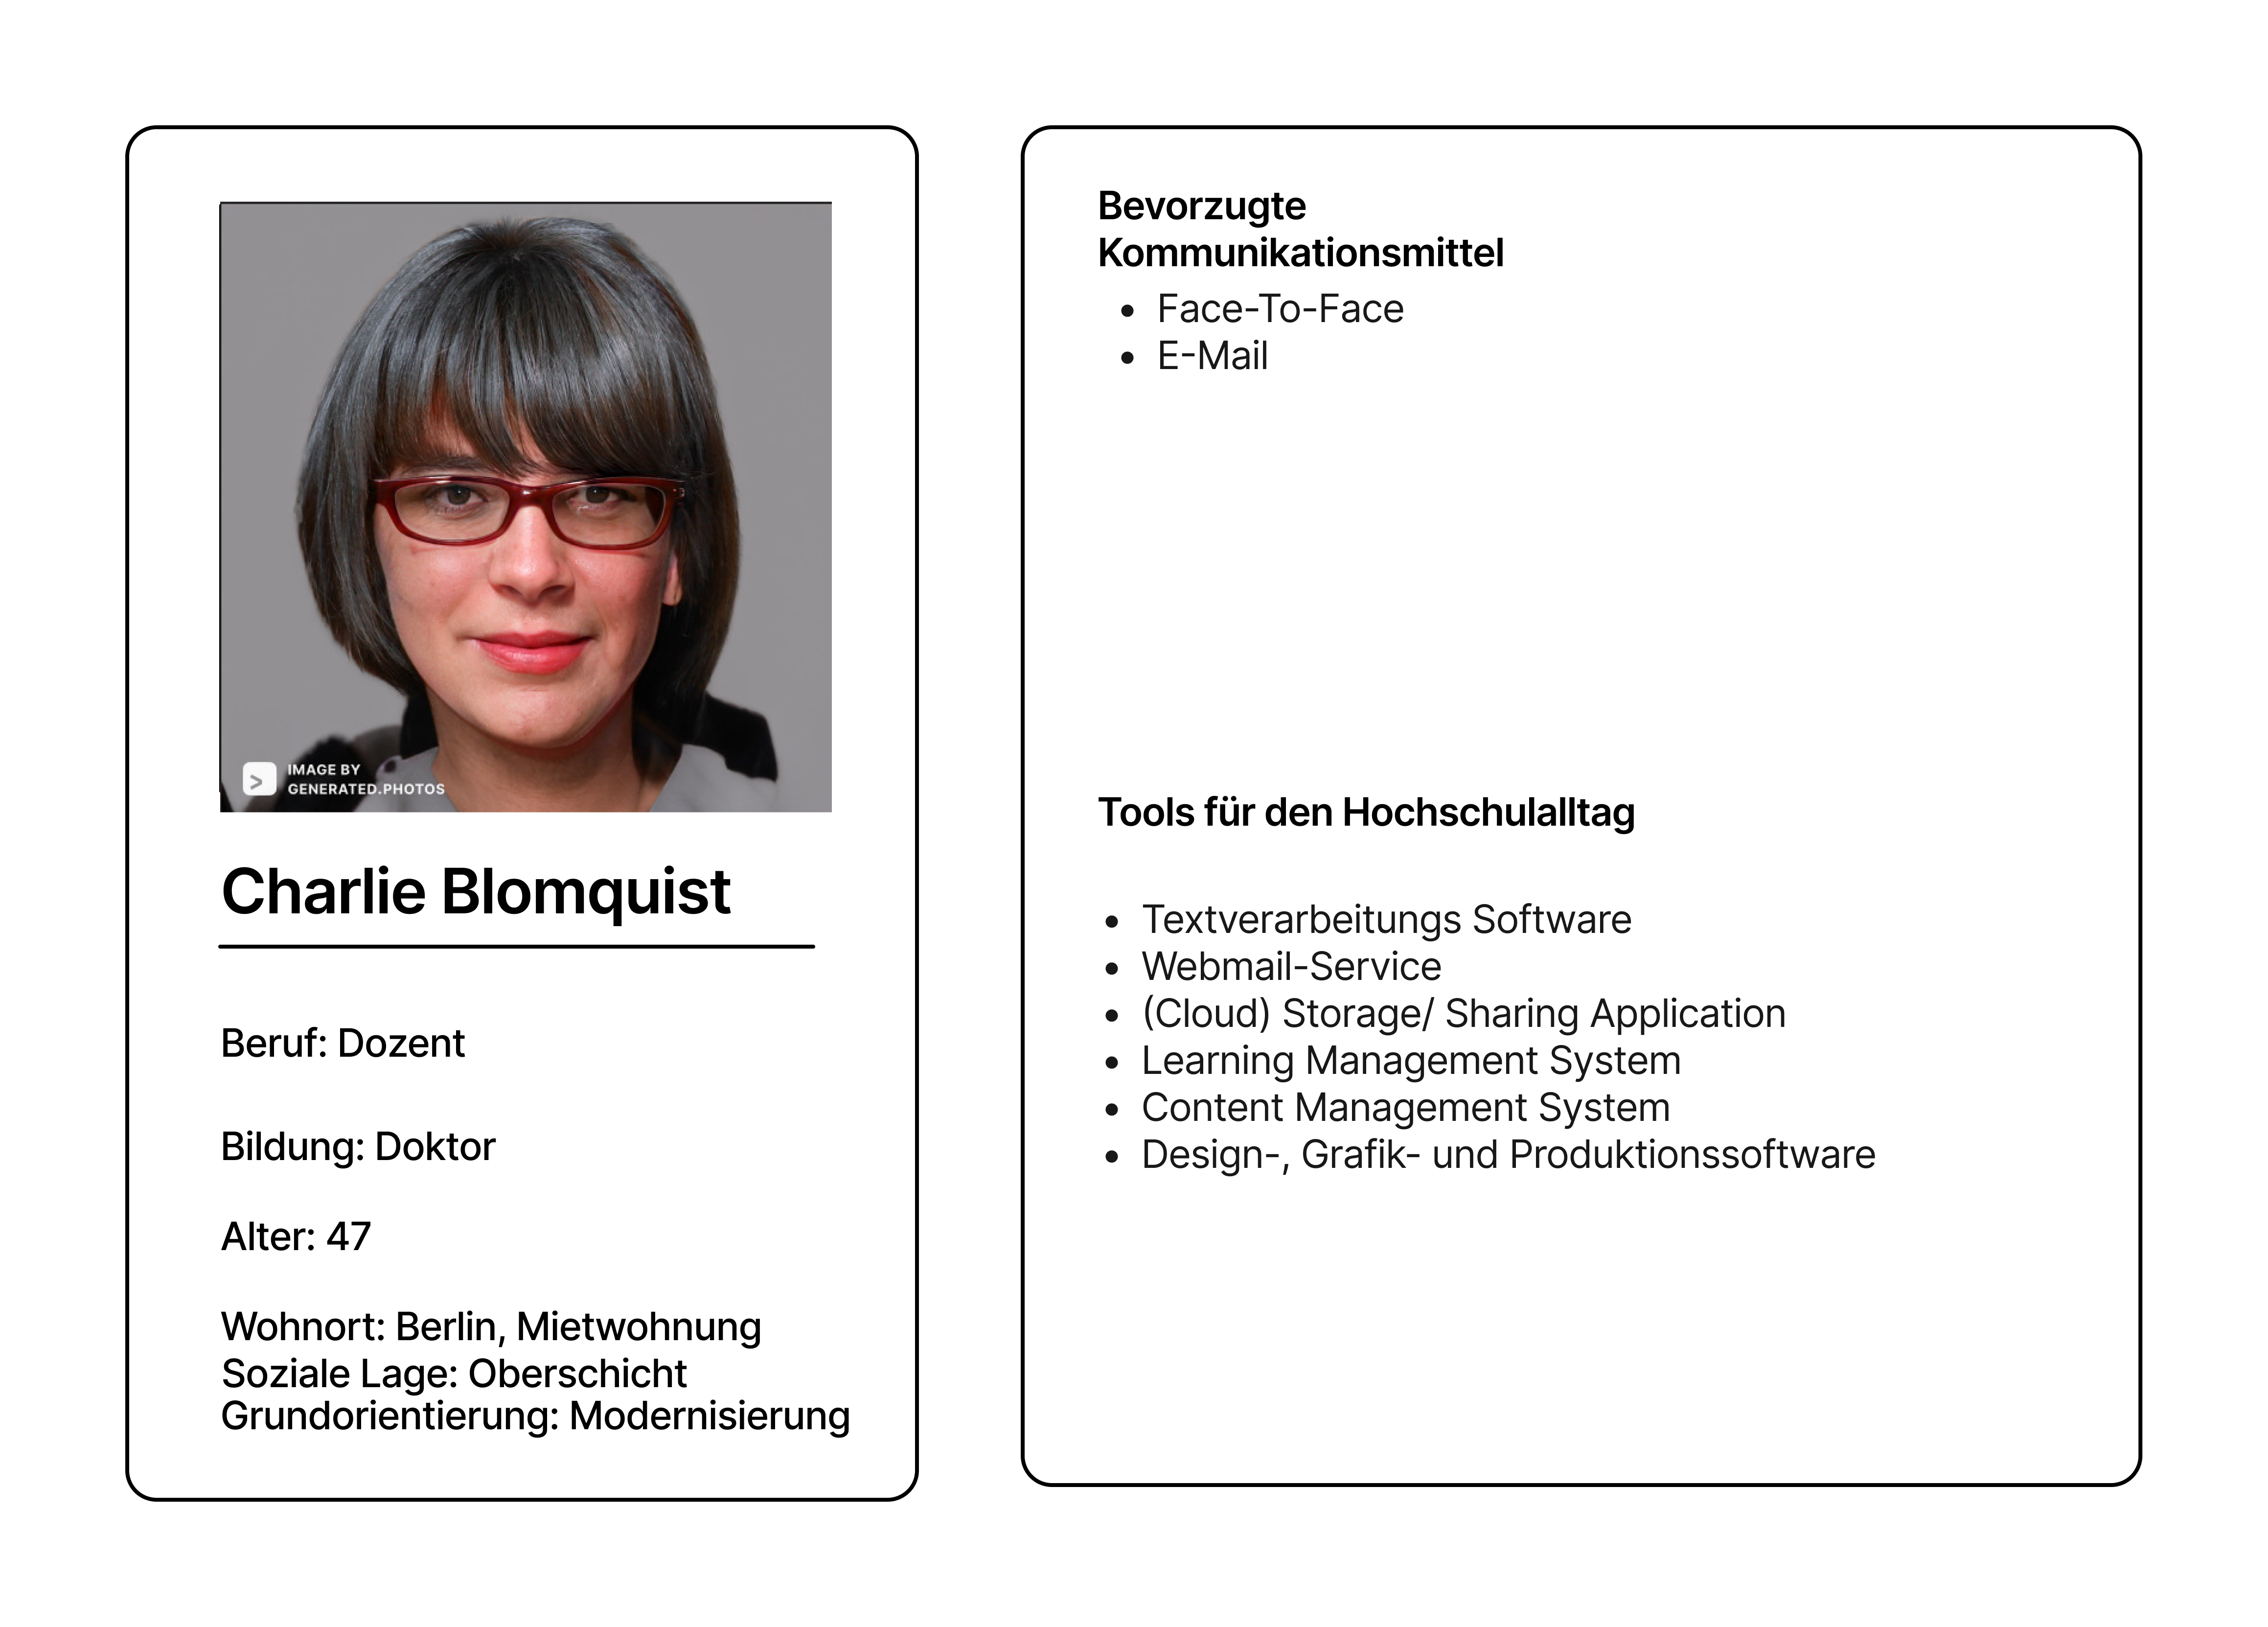
\includegraphics[width=0.95\textwidth]{persona-a-overview.png}
    \caption{Kurzvorstellung Charlie Blomquist}
	\label{fig:personaashort}
\end{figure}

\begin{figure}[H]
	\centering
	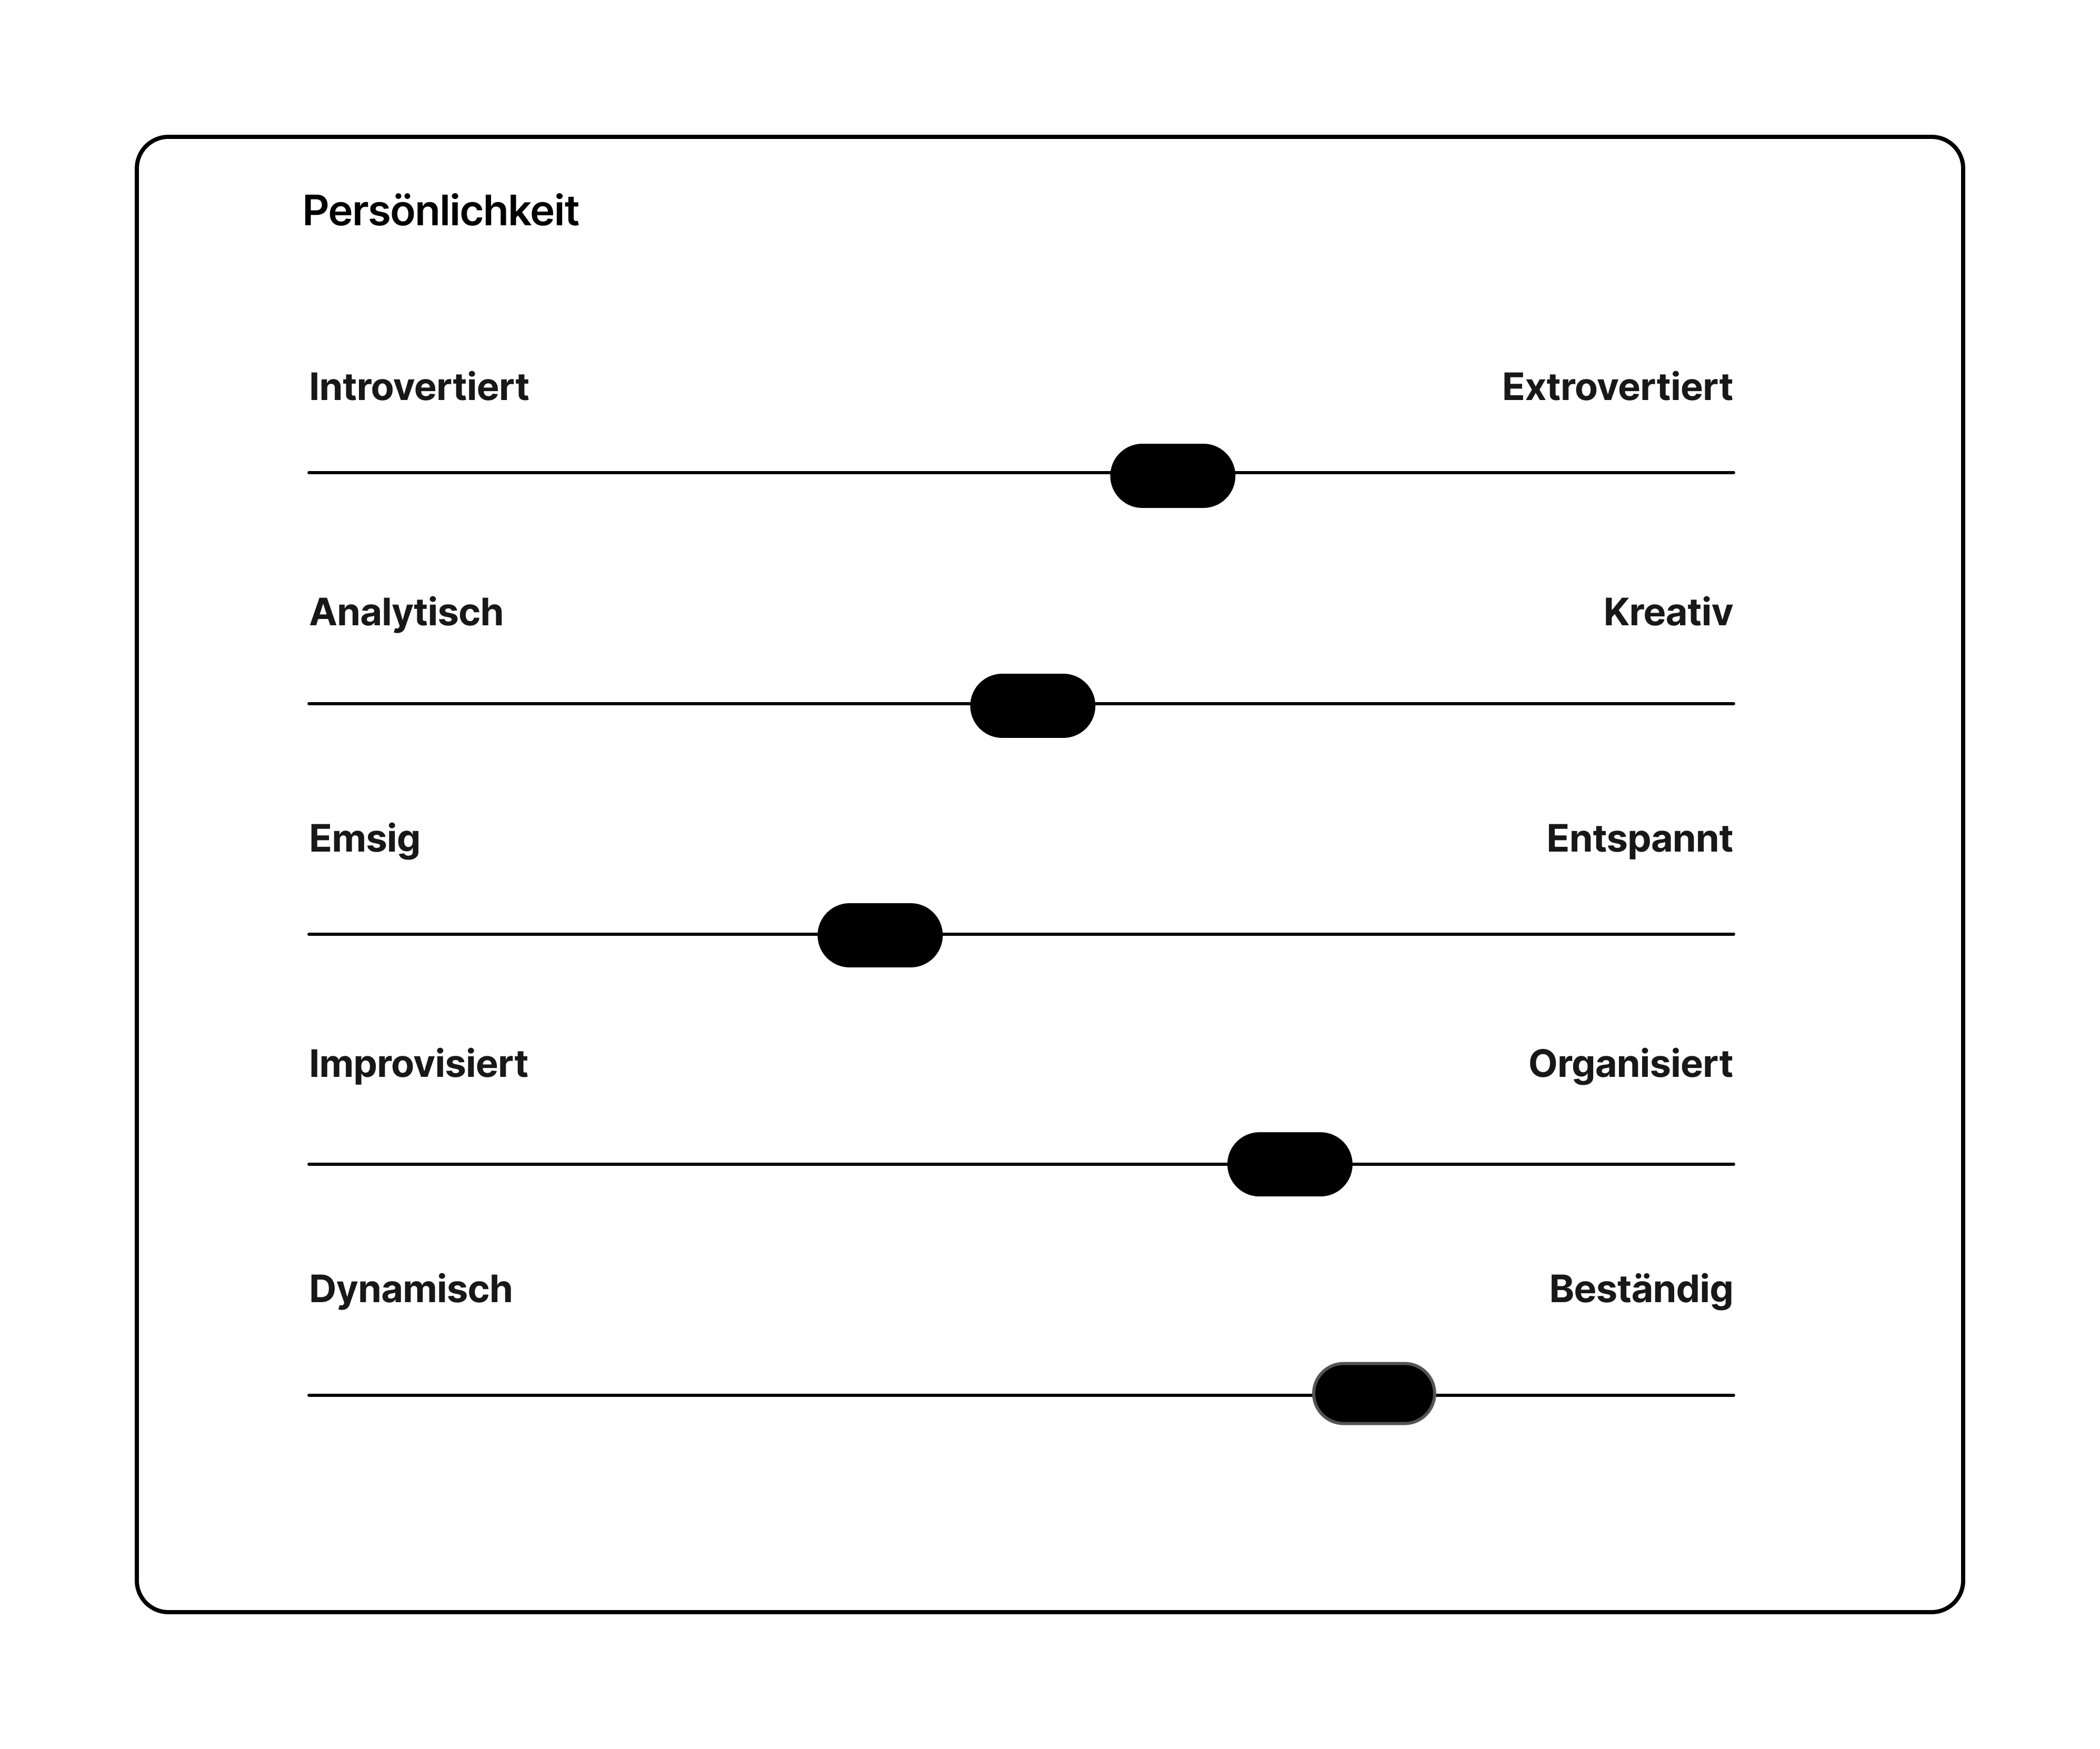
\includegraphics[width=0.95\textwidth]{persona-a-personality.png}
    \caption{Persönlichkeitszüge von Charlie Blomquist}
	\label{fig:personaapers}
\end{figure}

\begin{figure}[H]
	\centering
	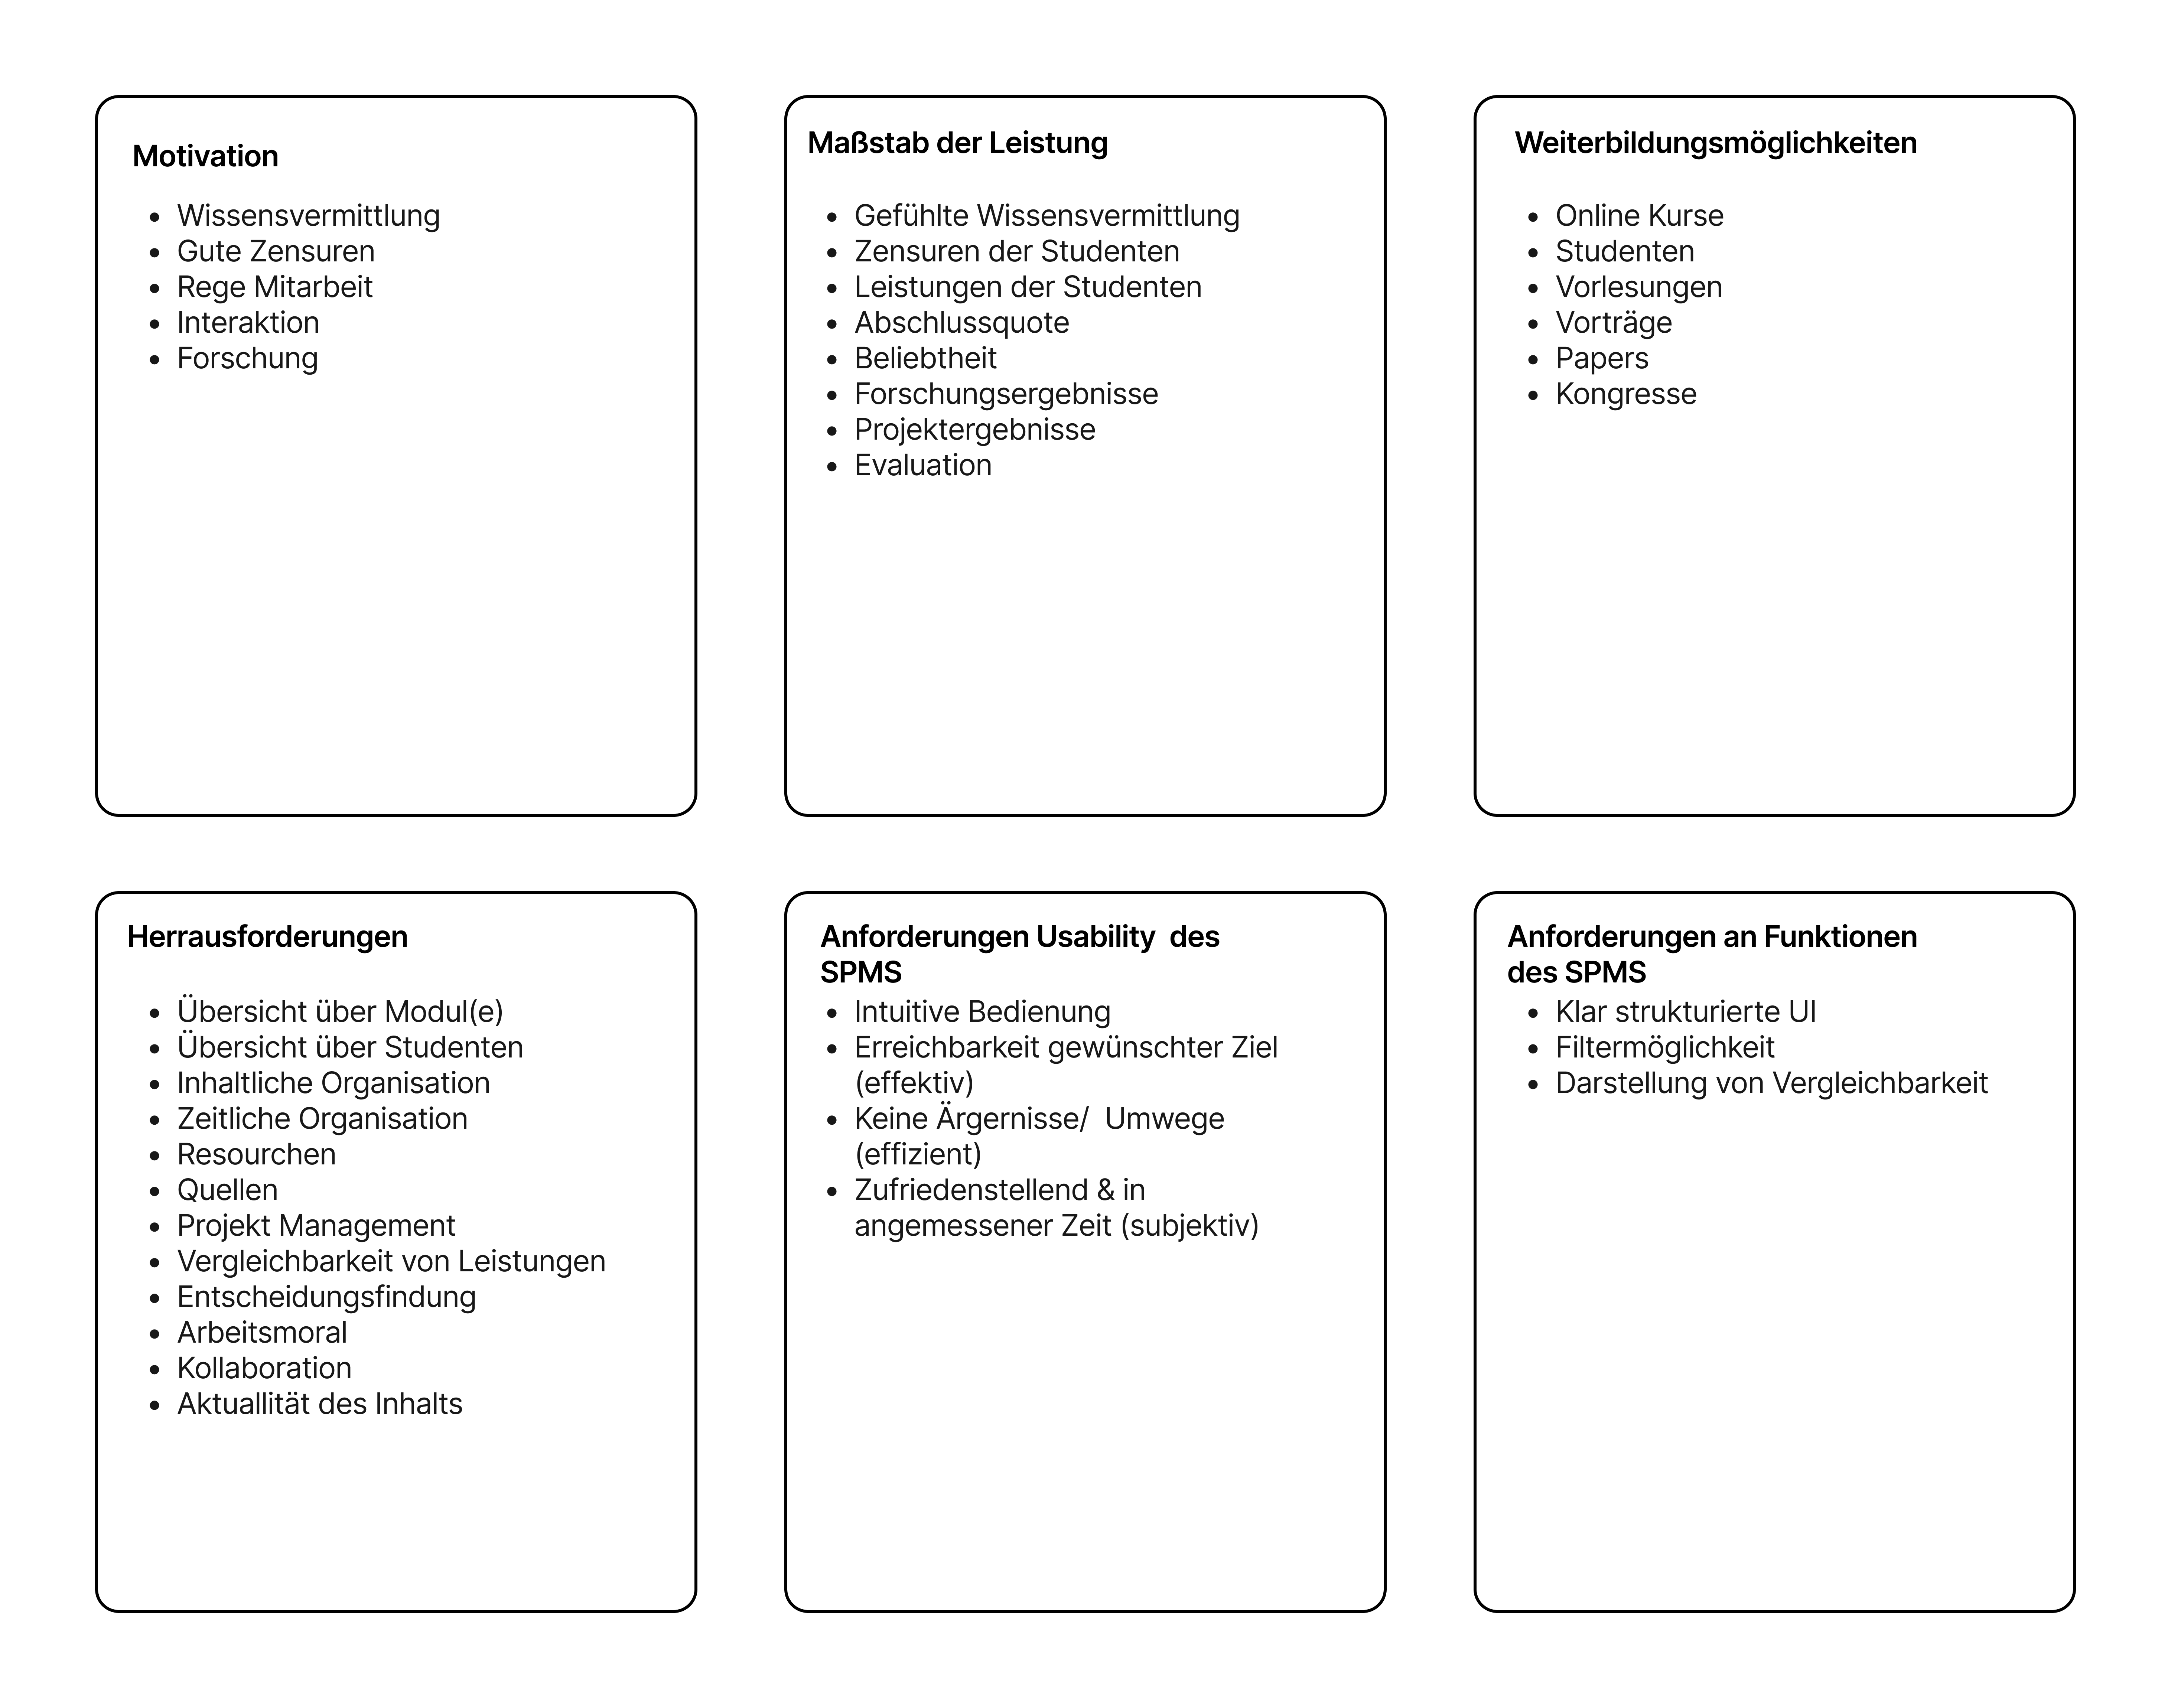
\includegraphics[width=0.95\textwidth]{persona-a-further.png}
    \caption{Weitere Informationen zu Chalie Blomquist}
	\label{fig:personaafurther}
\end{figure}

\section{Persona B: Kai Lind}

\begin{figure}[H]
	\centering
	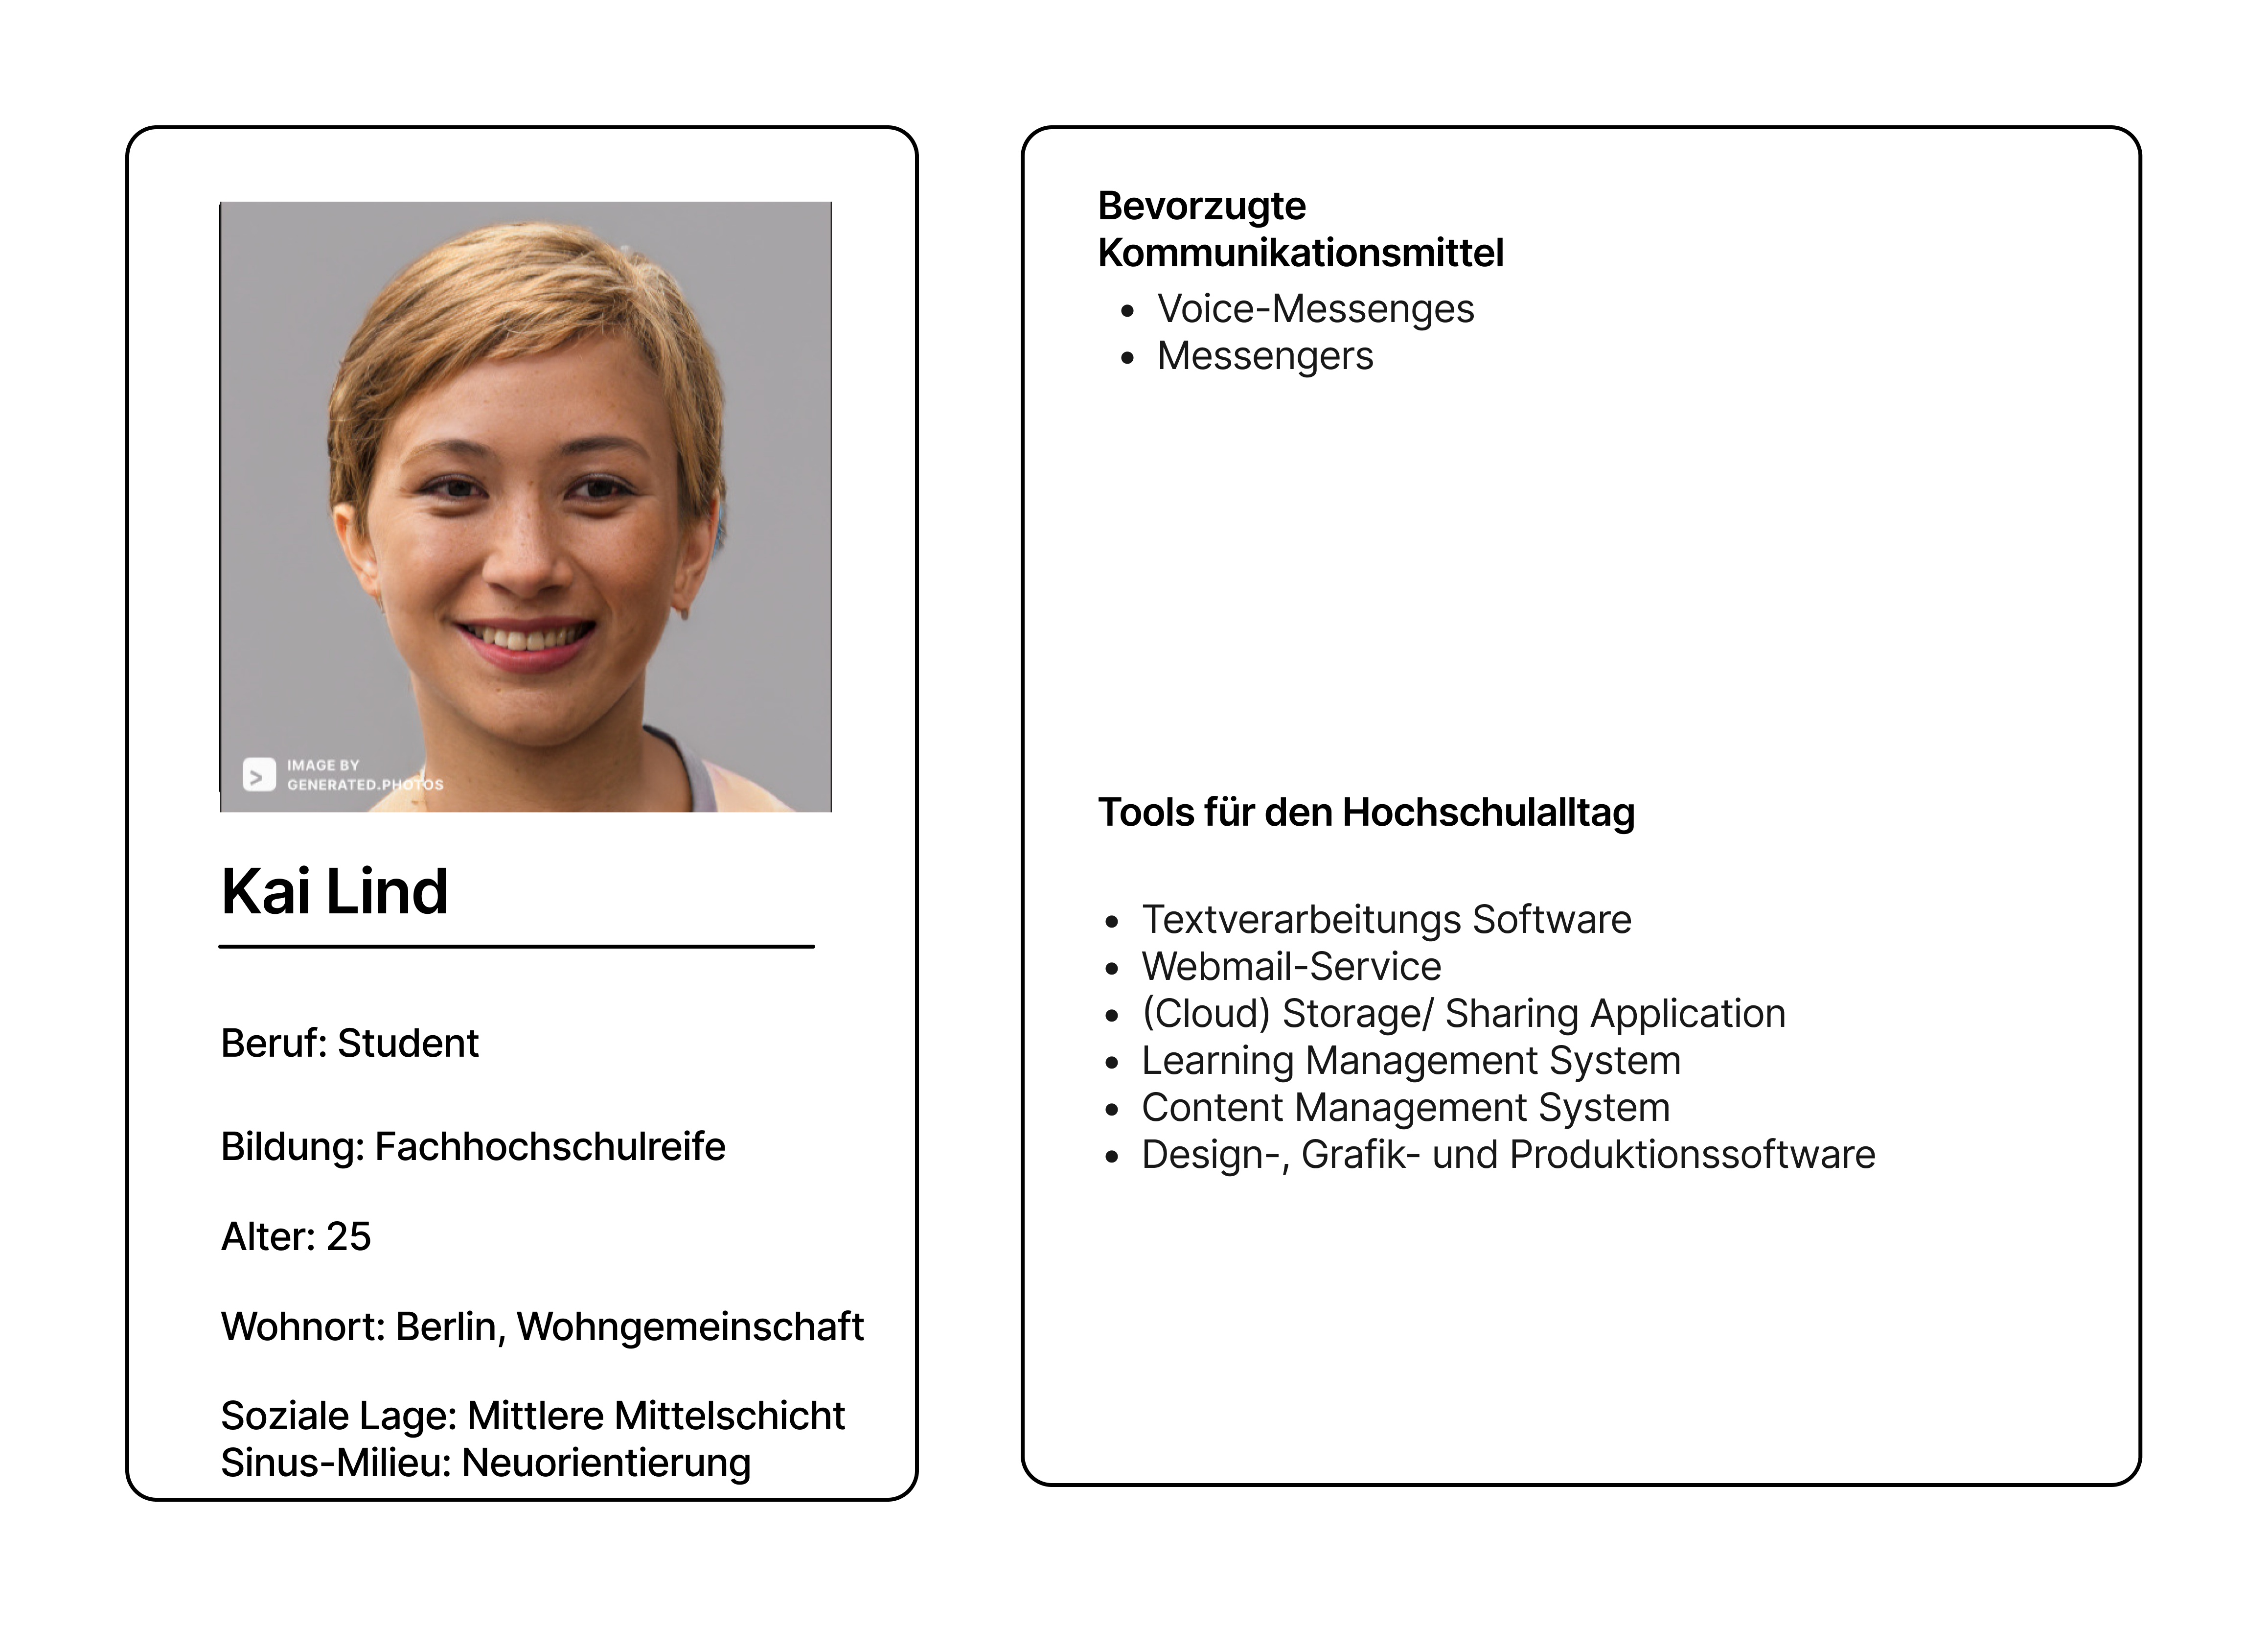
\includegraphics[width=0.95\textwidth]{persona-b-overview.png}
    \caption{Kurzvorstellung Kai Lind}
	\label{fig:personabshort}
\end{figure}

\begin{figure}[H]
	\centering
	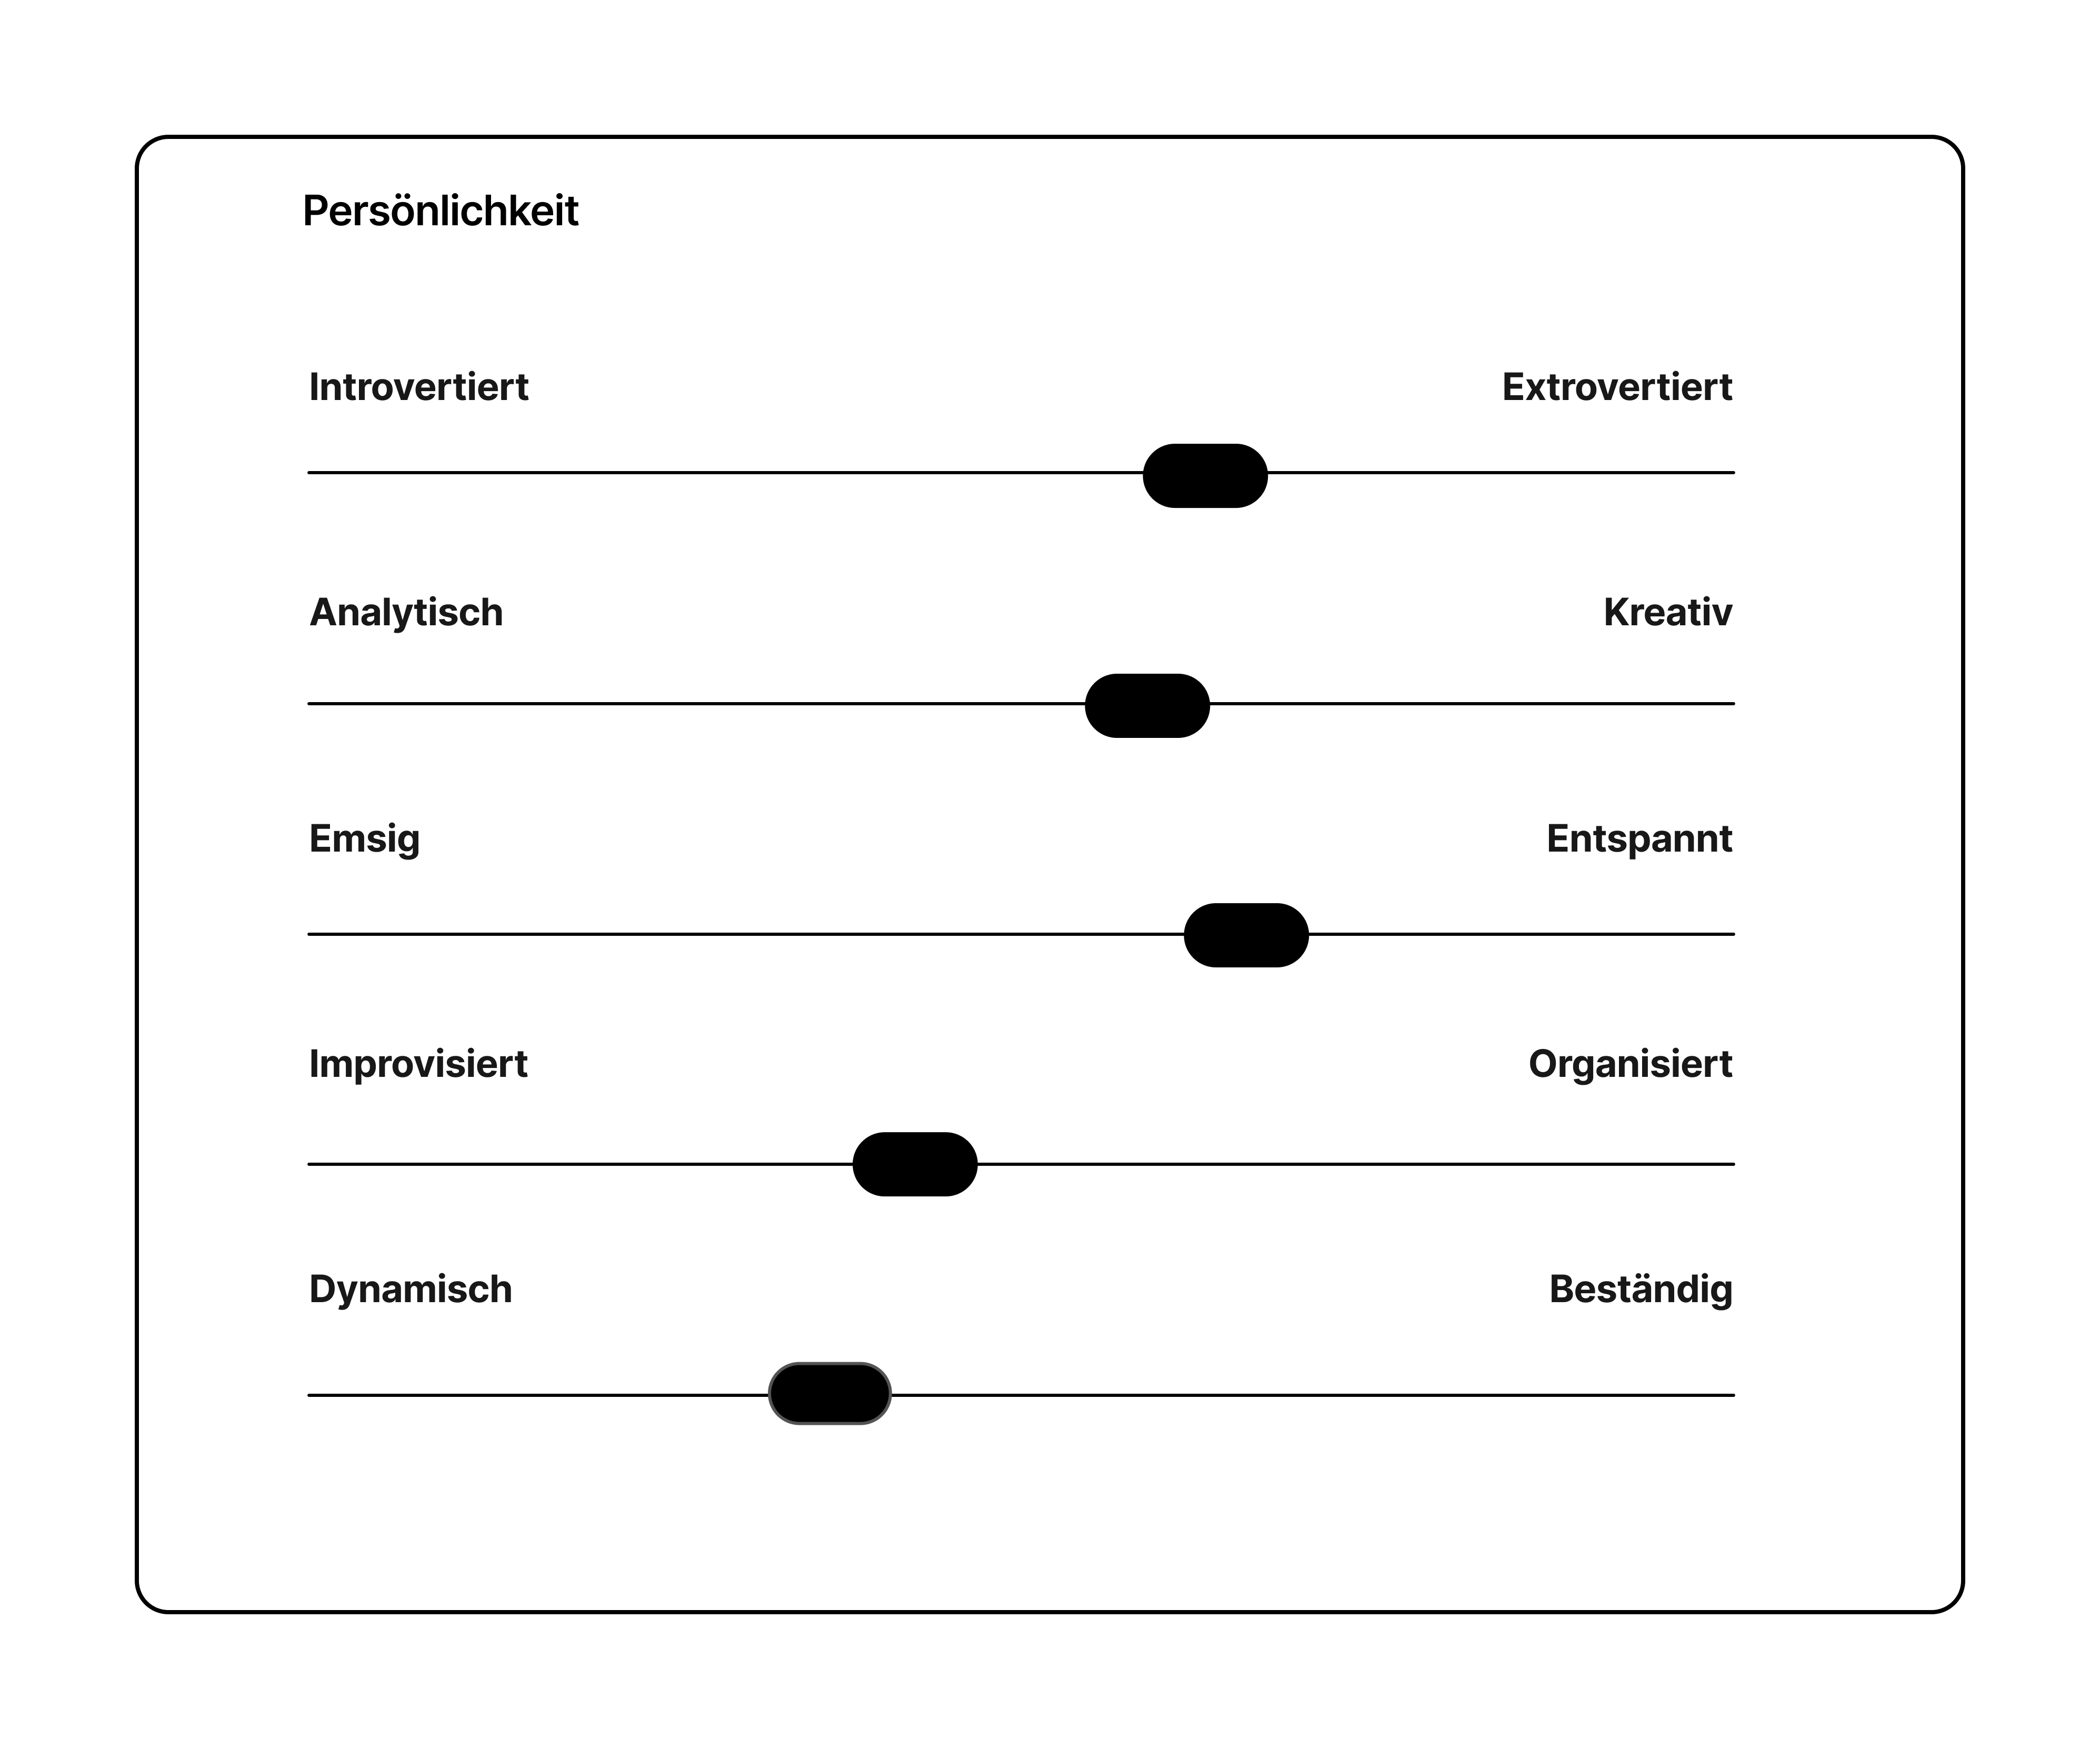
\includegraphics[width=0.95\textwidth]{persona-b-personality.png}
    \caption{Persönlichkeitszüge von Kai Lind}
	\label{fig:personabpers}
\end{figure}

\begin{figure}[H]
	\centering
	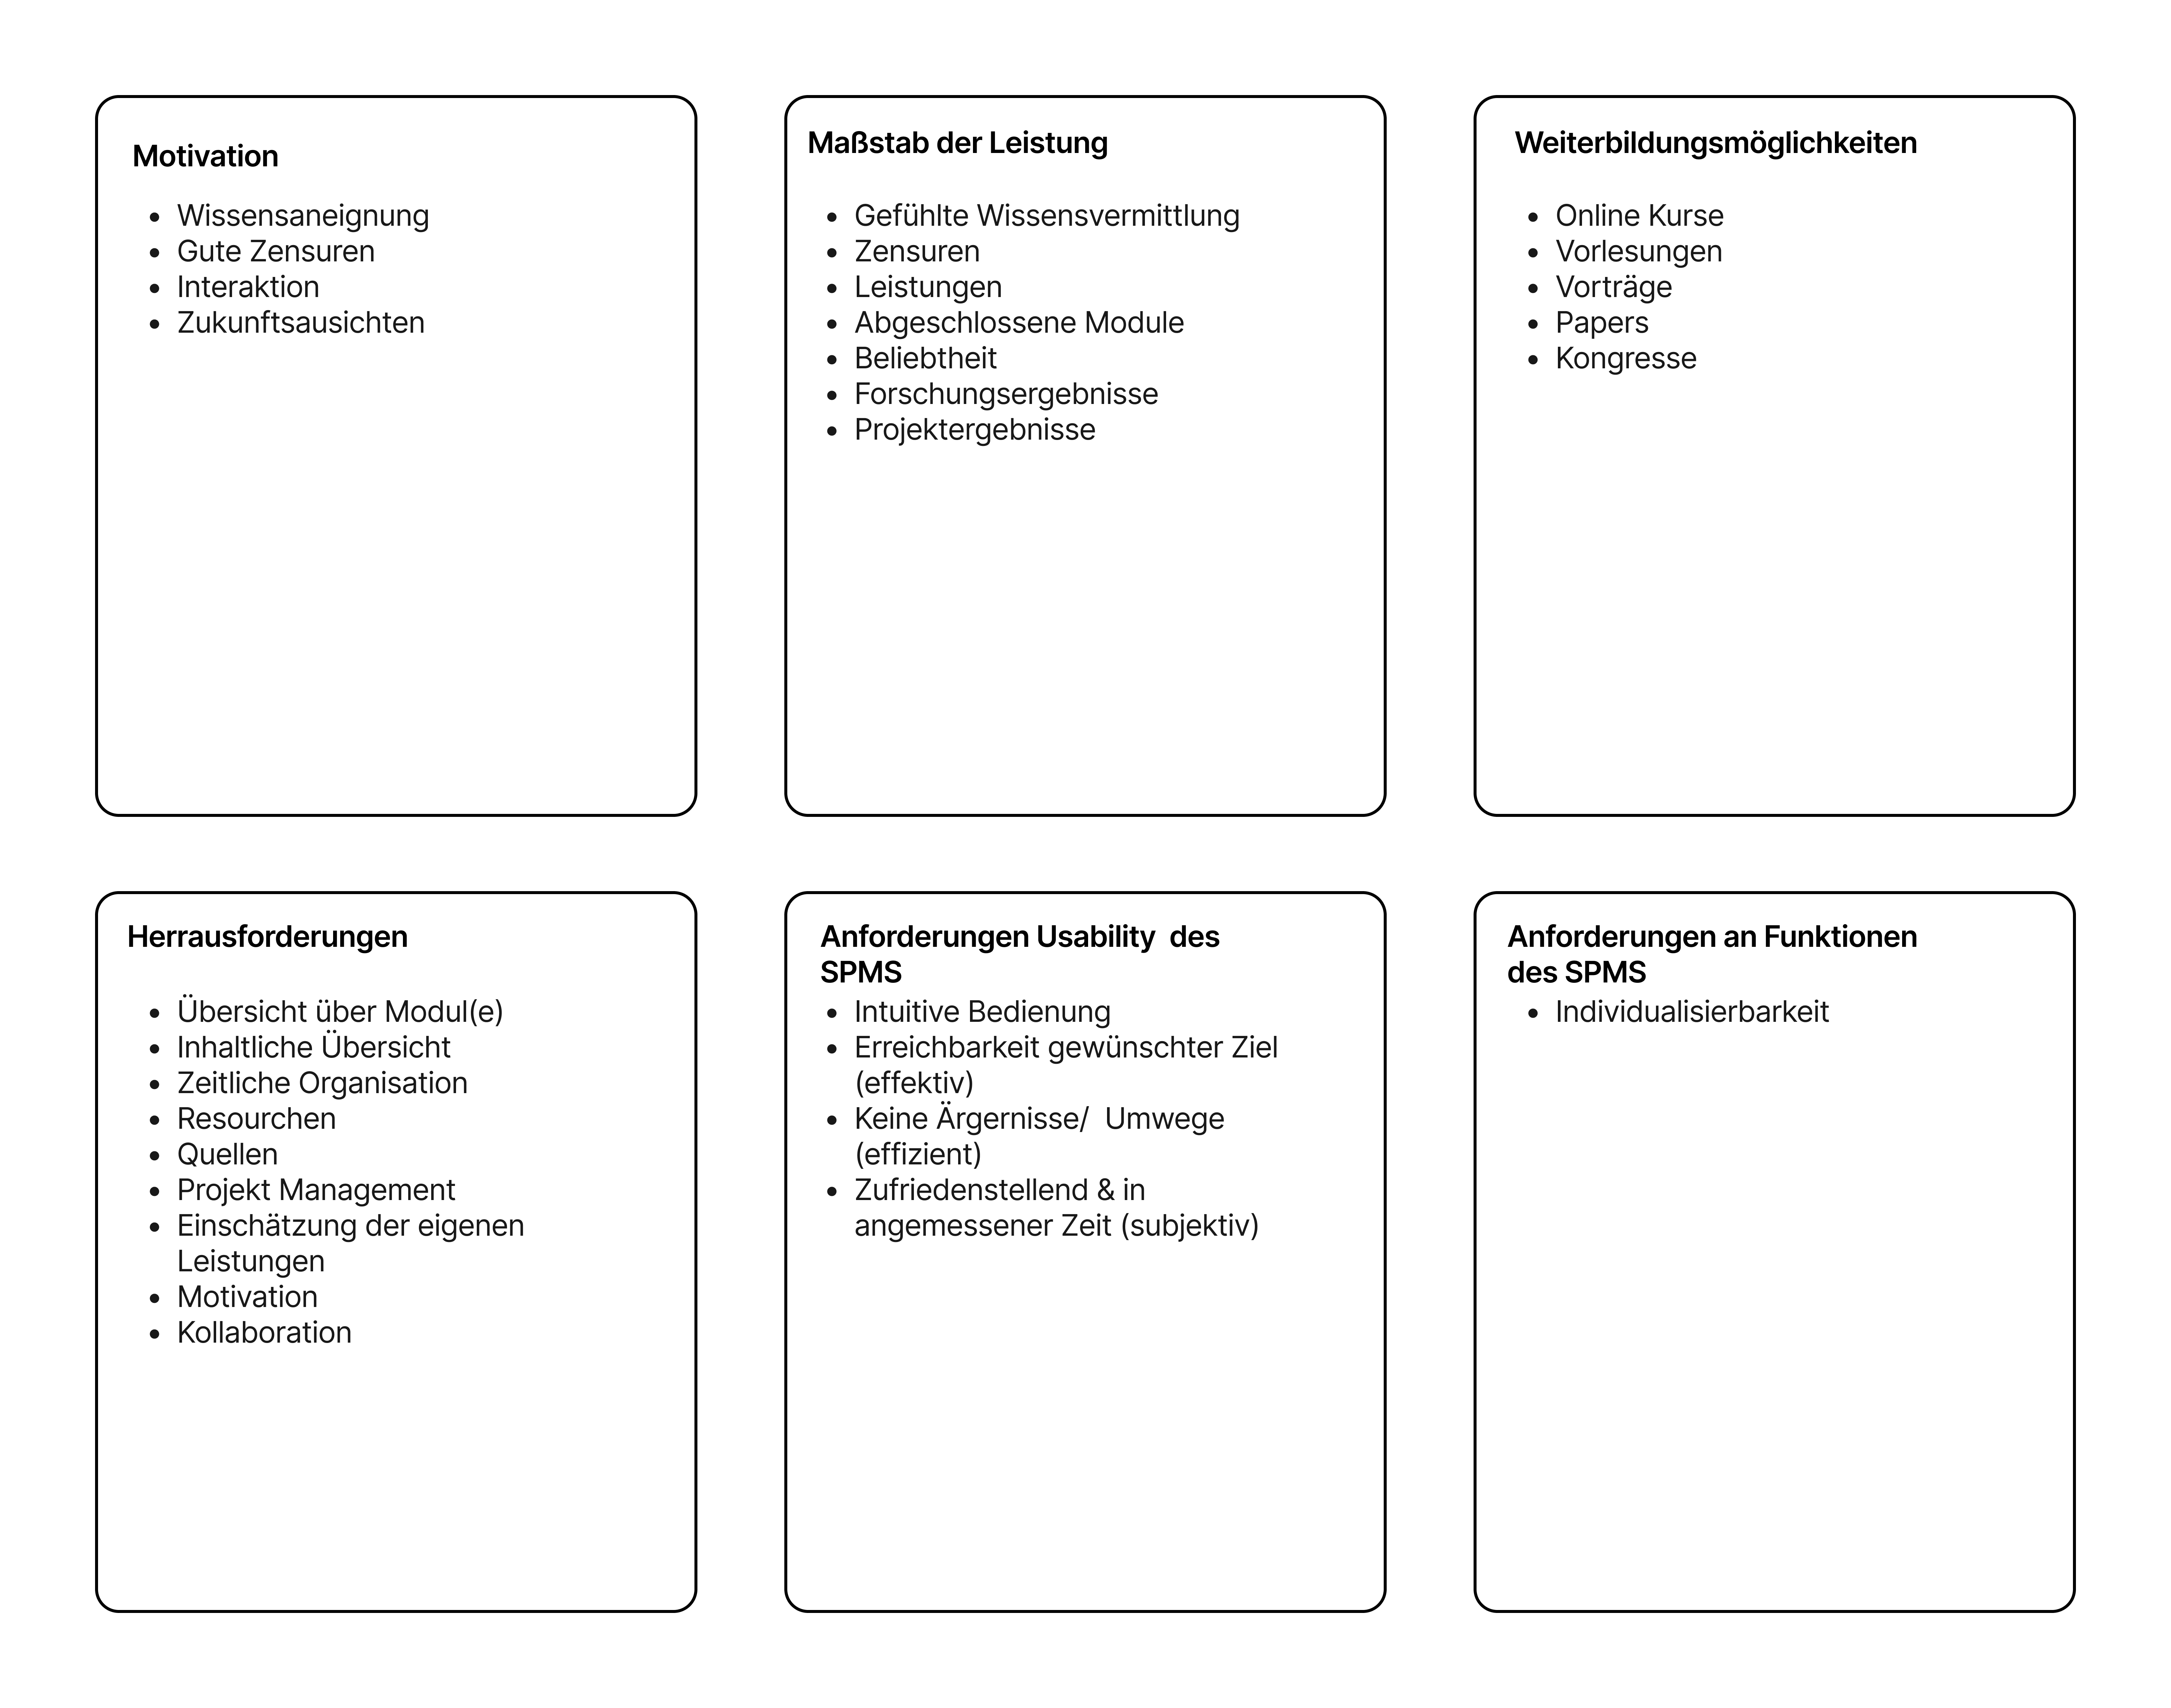
\includegraphics[width=0.95\textwidth]{persona-b-further.png}
    \caption{Weitere Informationen zu Kai Lind}
	\label{fig:personabfurther}
\end{figure}


\section{Hintergrund zu Personas}

Literatur\\
- \href{https://www.researchgate.net/publication/215500610_Personas_From_Theory_to_Practices}\\
- ...\\

Personas sind, im Bereich \ac{MCI}, ein häufig genutztes Mittel im Anforderungsmanagement um die Zielgruppe einer Anwendung genauer zu definieren. Sie dienen dazu während des Designprozesses Motivationen und Bedürfnisse möglicher Nutzer besser zu antizipieren und frühzeitig zu berücksichtigen.


	\chapter{Interviews}

Um Bedürfnisse realer Benutzer von vorne herein zu Berücksichtigen haben wir mit Usern ein, durch ein Fragebogen begleitetes Interview durchgeführt.

\section{Fragebogen und Ergebnisse}

Folgende Informationen haben wir mittels eines Fragebogens abgefragt.

\subsection{Frage 1: Benutzt du Weekly Standups?}
\begin{figure}[H]
	\centering
	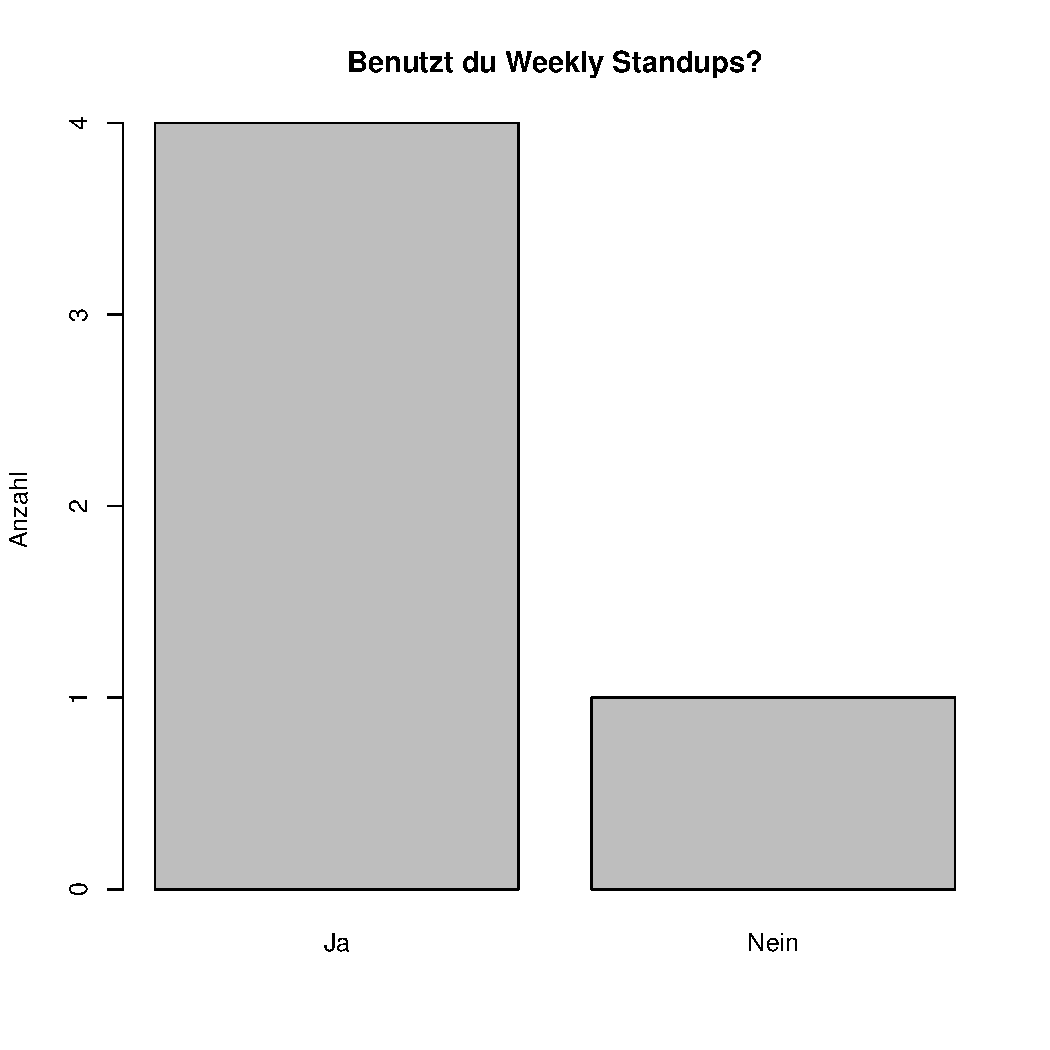
\includegraphics[width=0.60\textwidth]{q1.pdf}
    \caption{Verwendung von Weekly Standups unter den Befragten}
	\label{fig:q1}
\end{figure}

\subsection{Frage 2: Welcher Nutzergruppe gehörst du an?}
\begin{figure}[H]
	\centering
	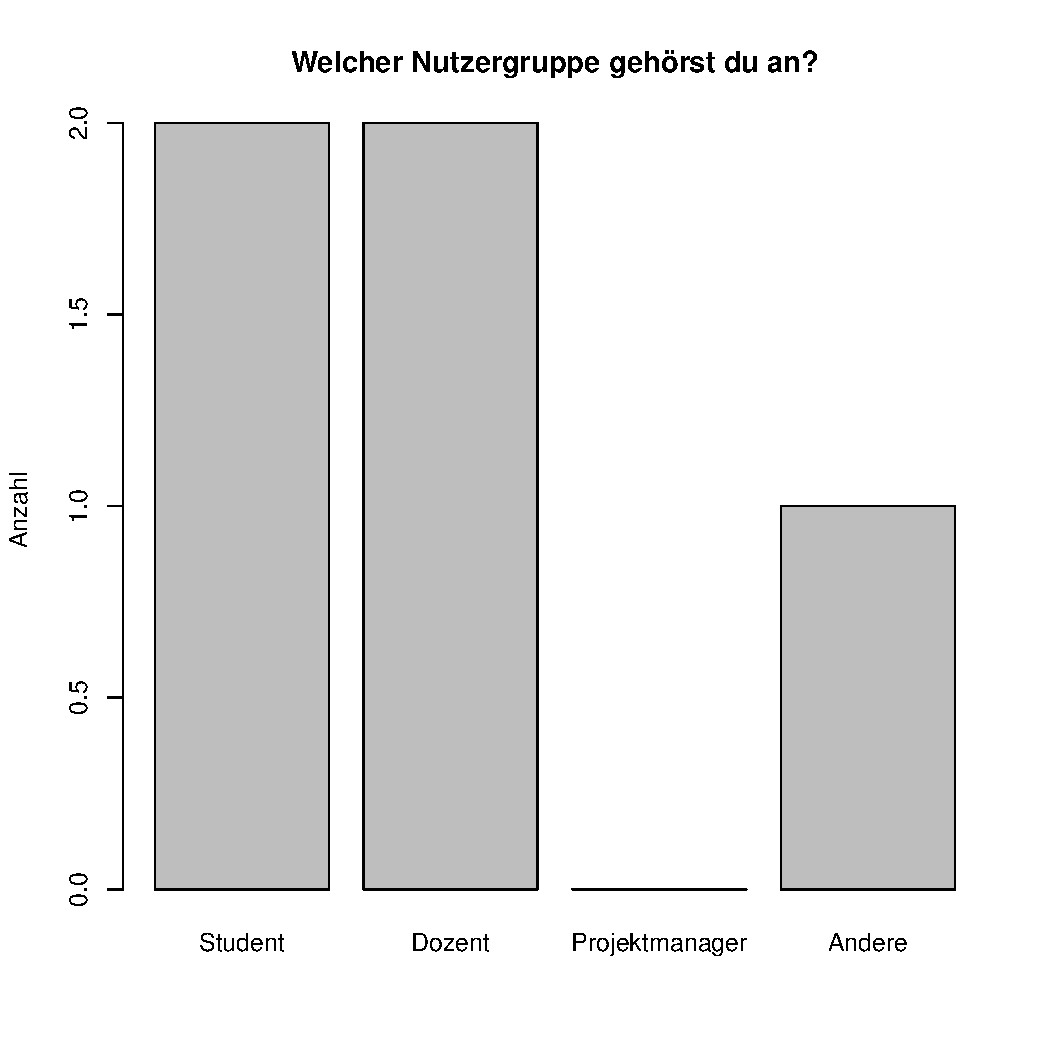
\includegraphics[width=0.60\textwidth]{q2.pdf}
    \caption{Nutzergruppe der Befragten}
	\label{fig:q2}
\end{figure}
\subsection{Frage 3: Welche Projektarten führst du aus?}
\begin{figure}[H]
	\centering
	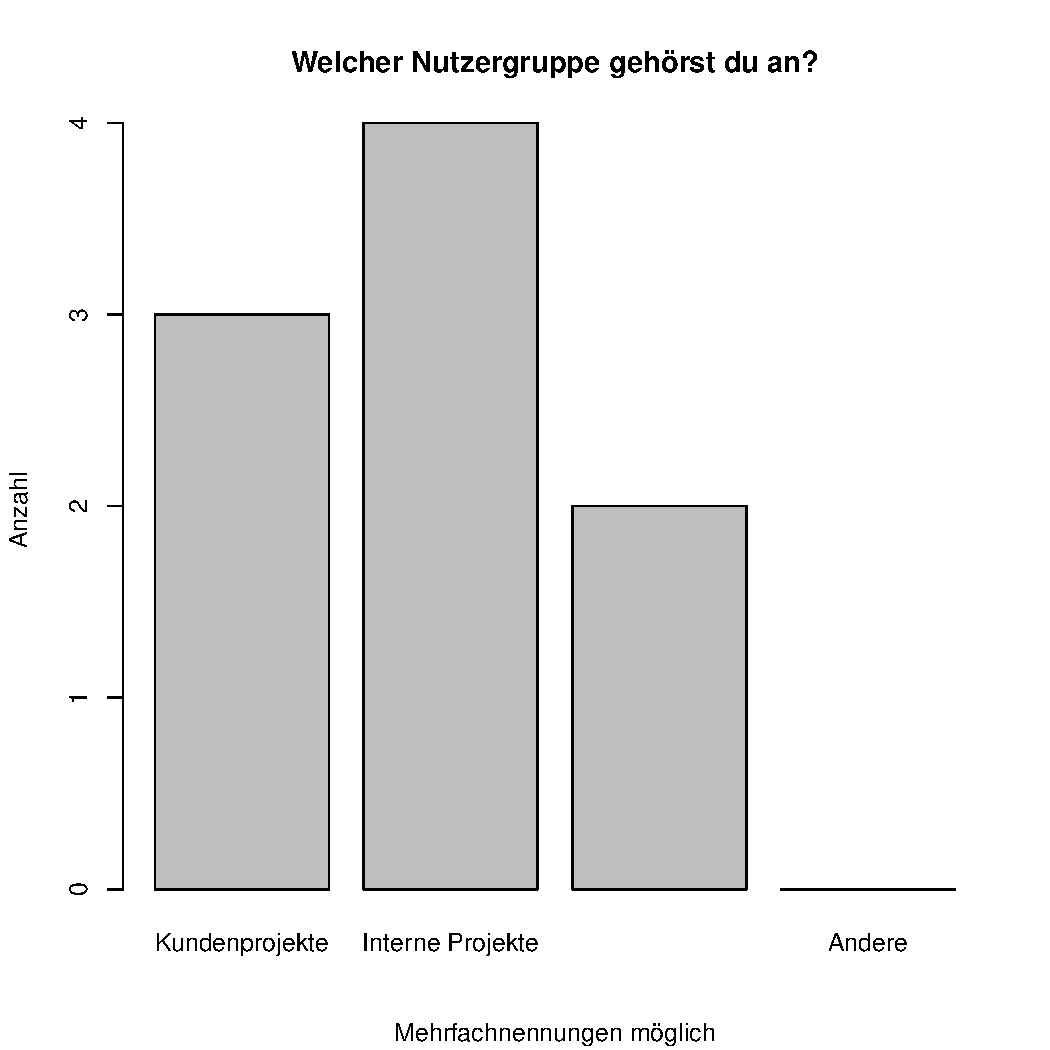
\includegraphics[width=0.60\textwidth]{q3.pdf}
    \caption{Projektarten der Befragten}
	\label{fig:q3}
\end{figure}
\subsection{Frage 4: Wie alt bist du?} 
\begin{figure}[H]
	\centering
	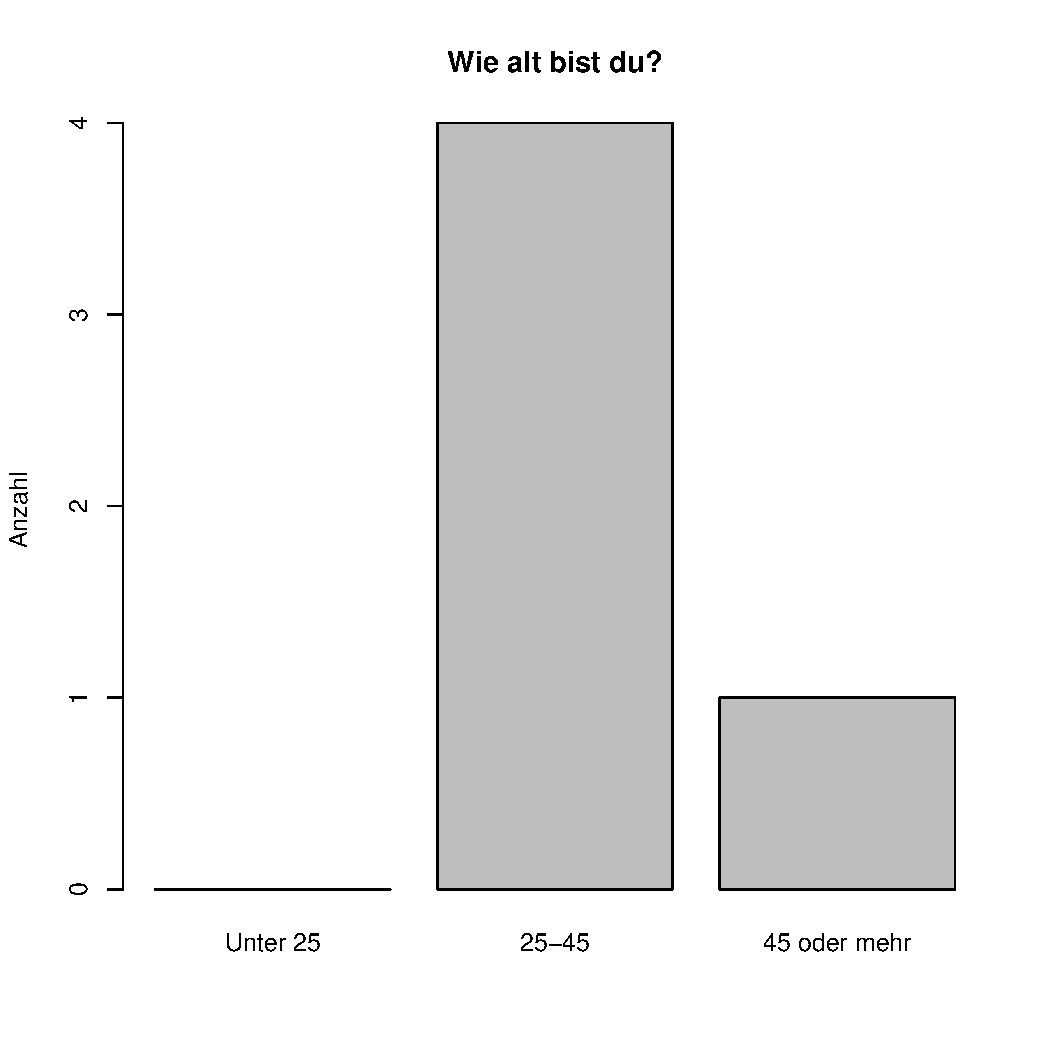
\includegraphics[width=0.60\textwidth]{q4.pdf}
    \caption{Alter der Befragten}
	\label{fig:q4}
\end{figure}     
\subsection{Frage 5: Wie viel Zeit verbringst du Wöchentlich in Standup Meetings?}
\begin{figure}[H]
	\centering
	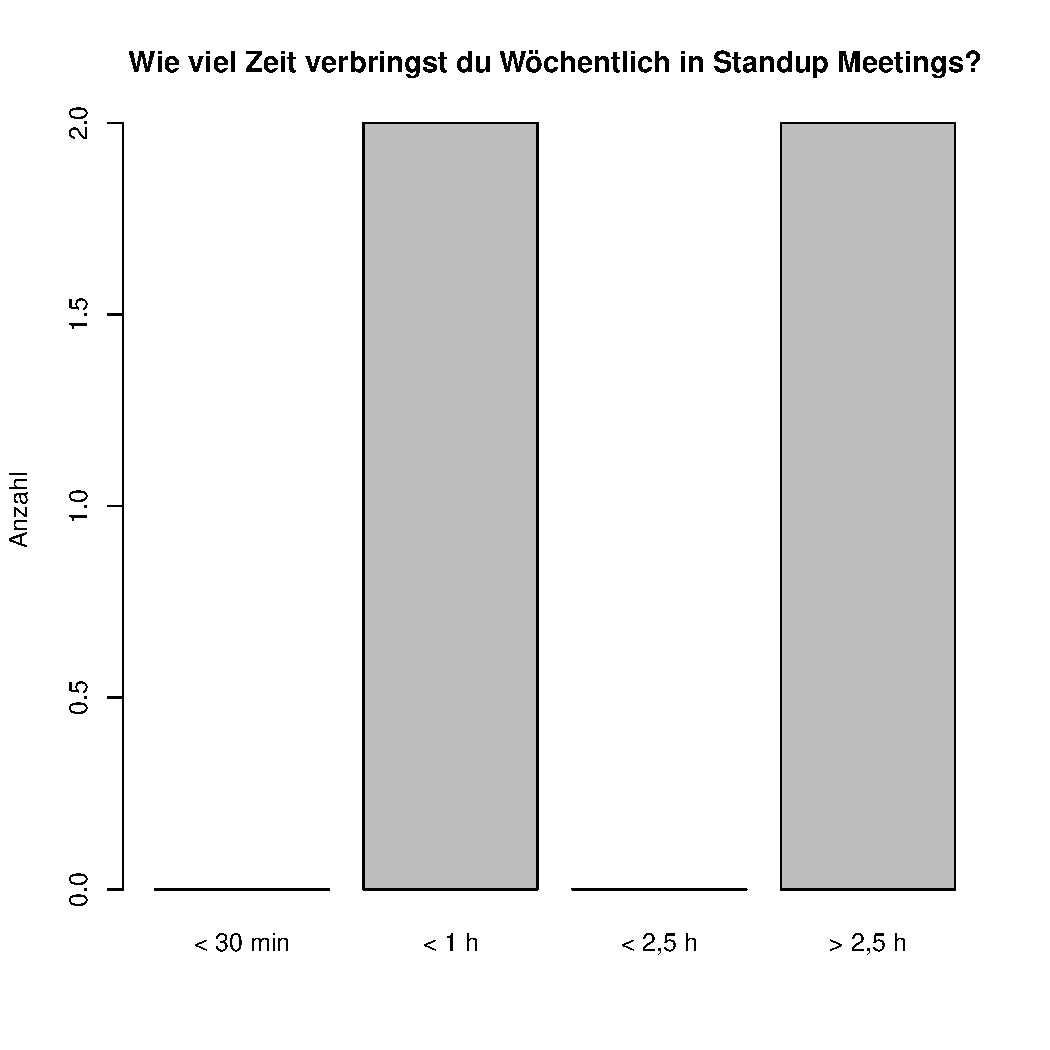
\includegraphics[width=0.60\textwidth]{q5.pdf}
    \caption{Zeit welche die Befragten in Statusmeetings verbringen}
	\label{fig:q5}
\end{figure}  
\subsection{Frage 6: Wie hilfreich findest du Weekly Standups?}
\begin{figure}[H]
	\centering
	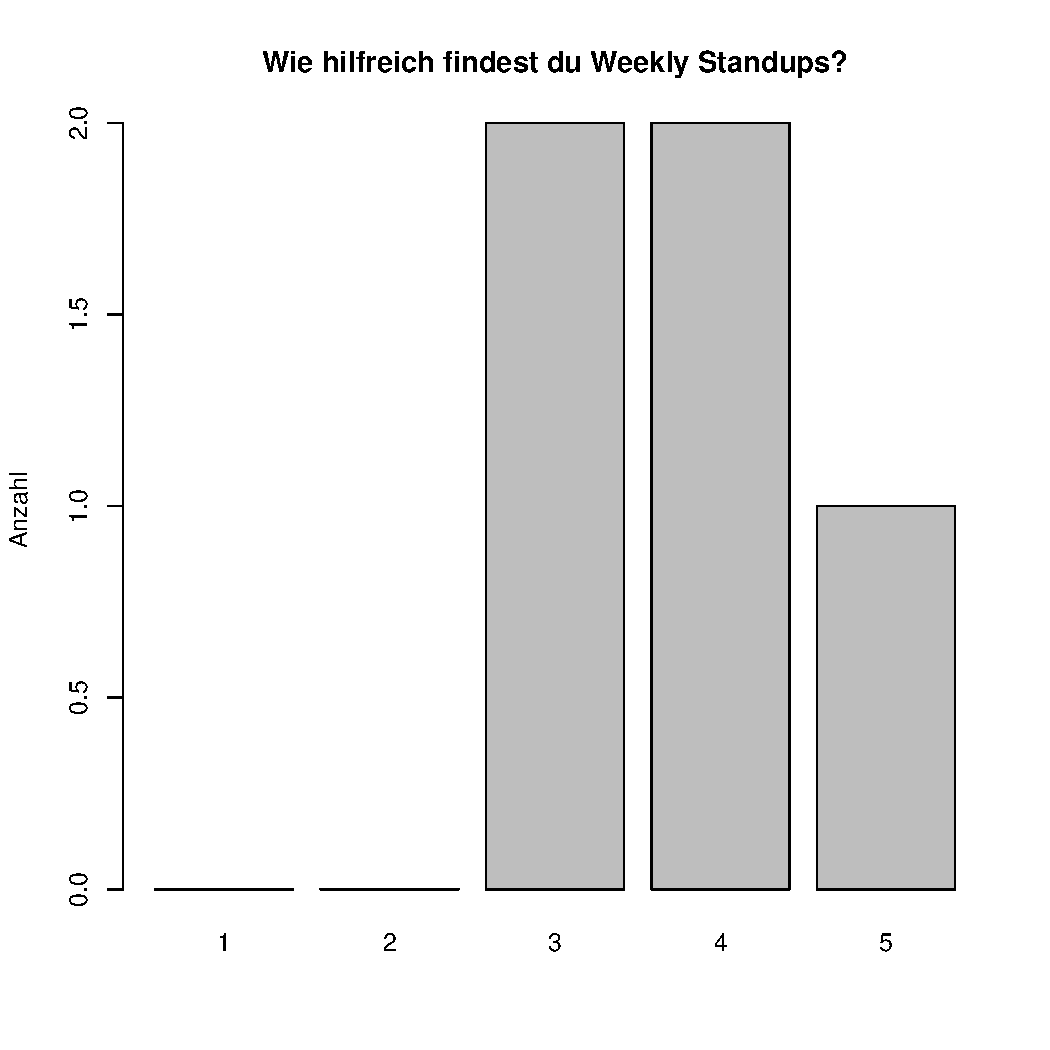
\includegraphics[width=0.60\textwidth]{q6.pdf}
    \caption{Gefühlter Nutzen eines Weekly Standups}
	\label{fig:q6}
\end{figure}  
\subsection{Frage 7: Wie arbeitest du zur Zeit?}
\begin{figure}[H]
	\centering
	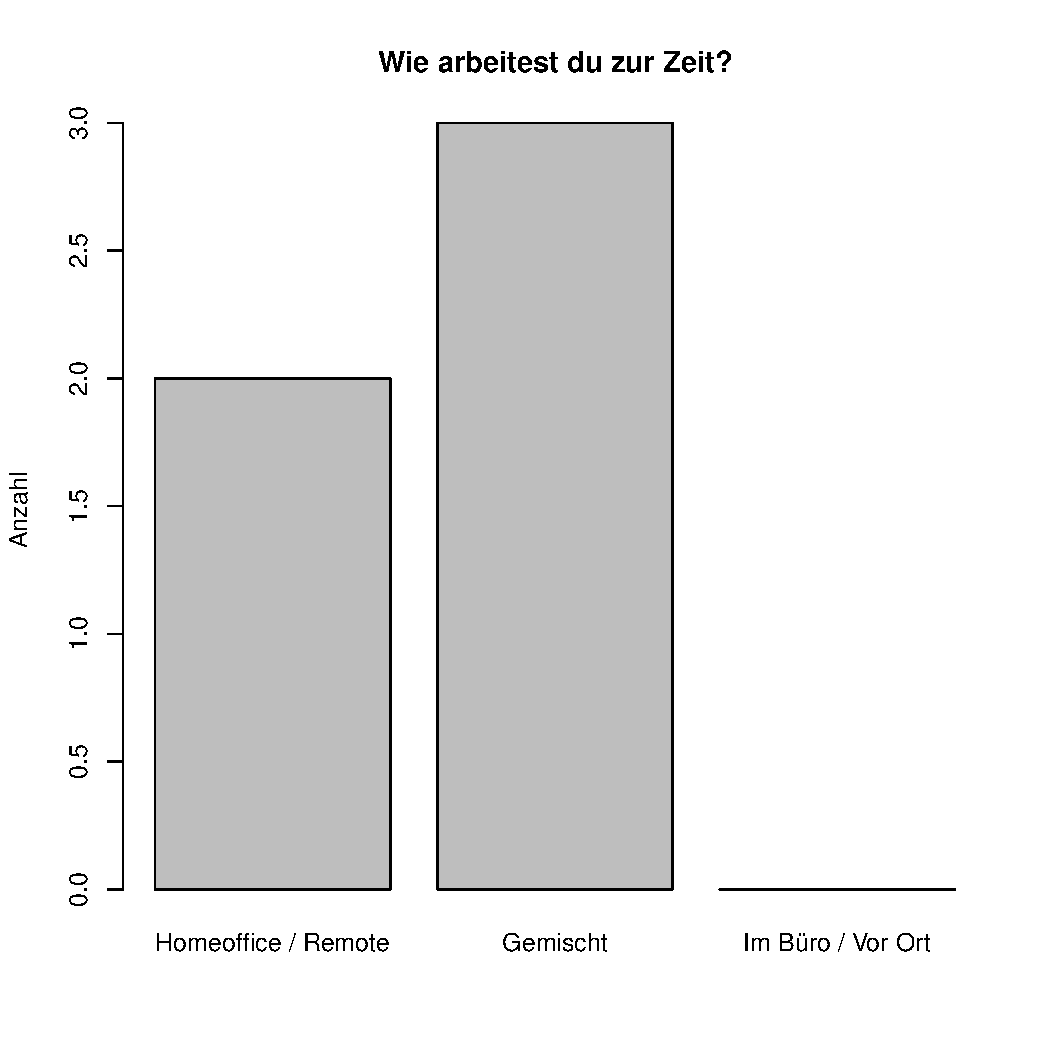
\includegraphics[width=0.60\textwidth]{q7.pdf}
    \caption{Arbeitsumfeld der Befragten}
	\label{fig:q7}
\end{figure}  
\subsection{Frage 8: Wie bewertest du folgende Features?}
\subsubsection{Frage 8.1: Erinnerung}
\begin{figure}[H]
	\centering
	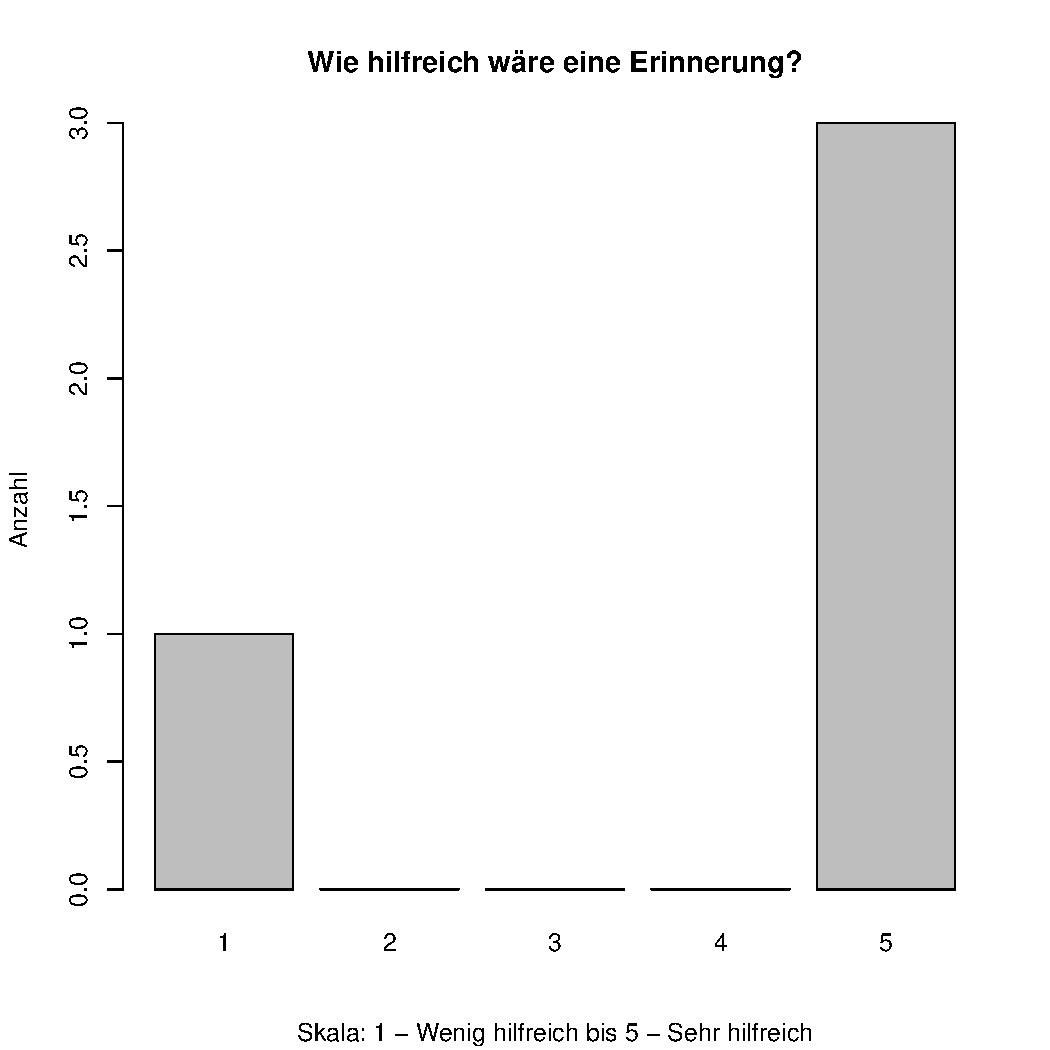
\includegraphics[width=0.60\textwidth]{q8-1.pdf}
    \caption{Nützlichkeit einer Erinnerung}
	\label{fig:q81}
\end{figure} 
\subsubsection{Frage 8.2: Timeline}
\begin{figure}[H]
	\centering
	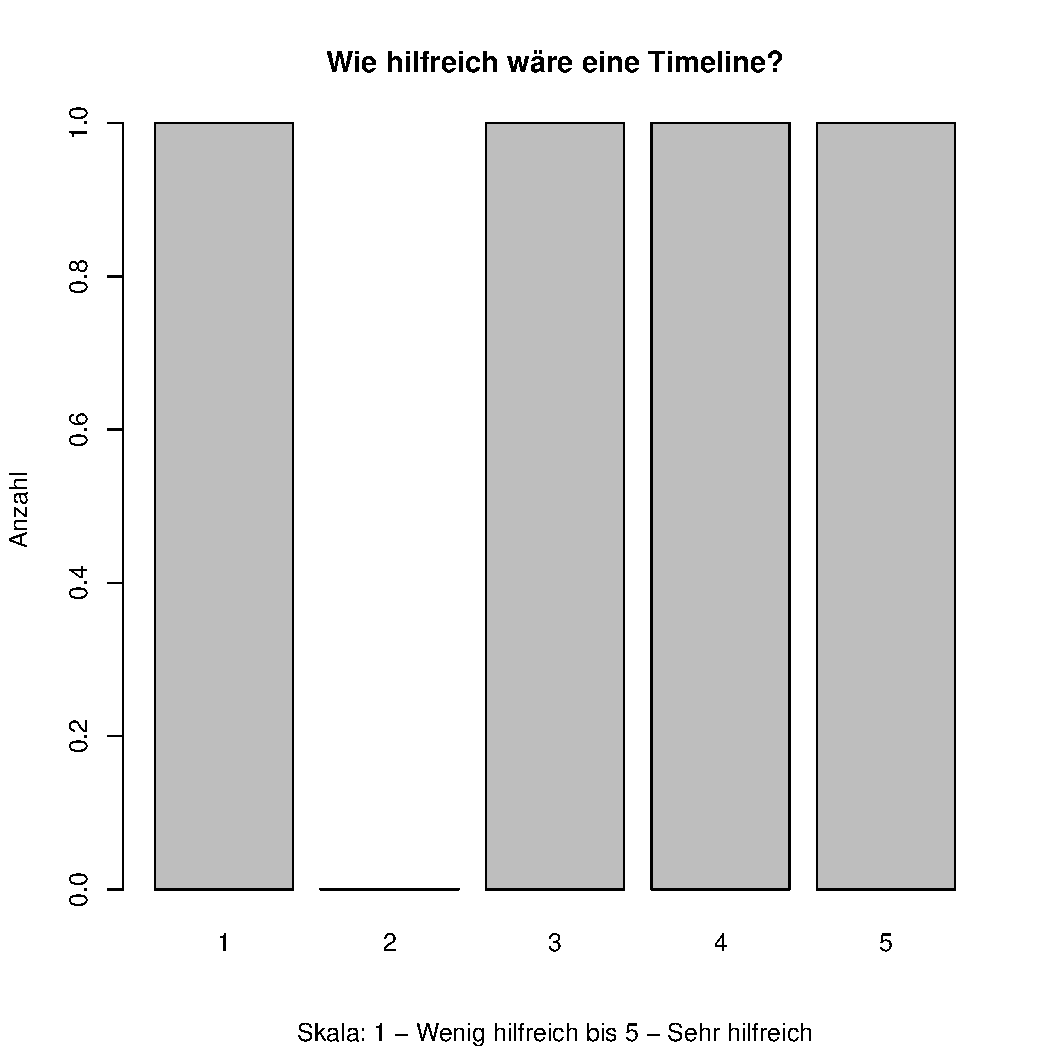
\includegraphics[width=0.60\textwidth]{q8-2.pdf}
    \caption{Nützlichkeit einer Timeline}
	\label{fig:q82}
\end{figure} 
\subsubsection{Frage 8.3: Suche}
\begin{figure}[H]
	\centering
	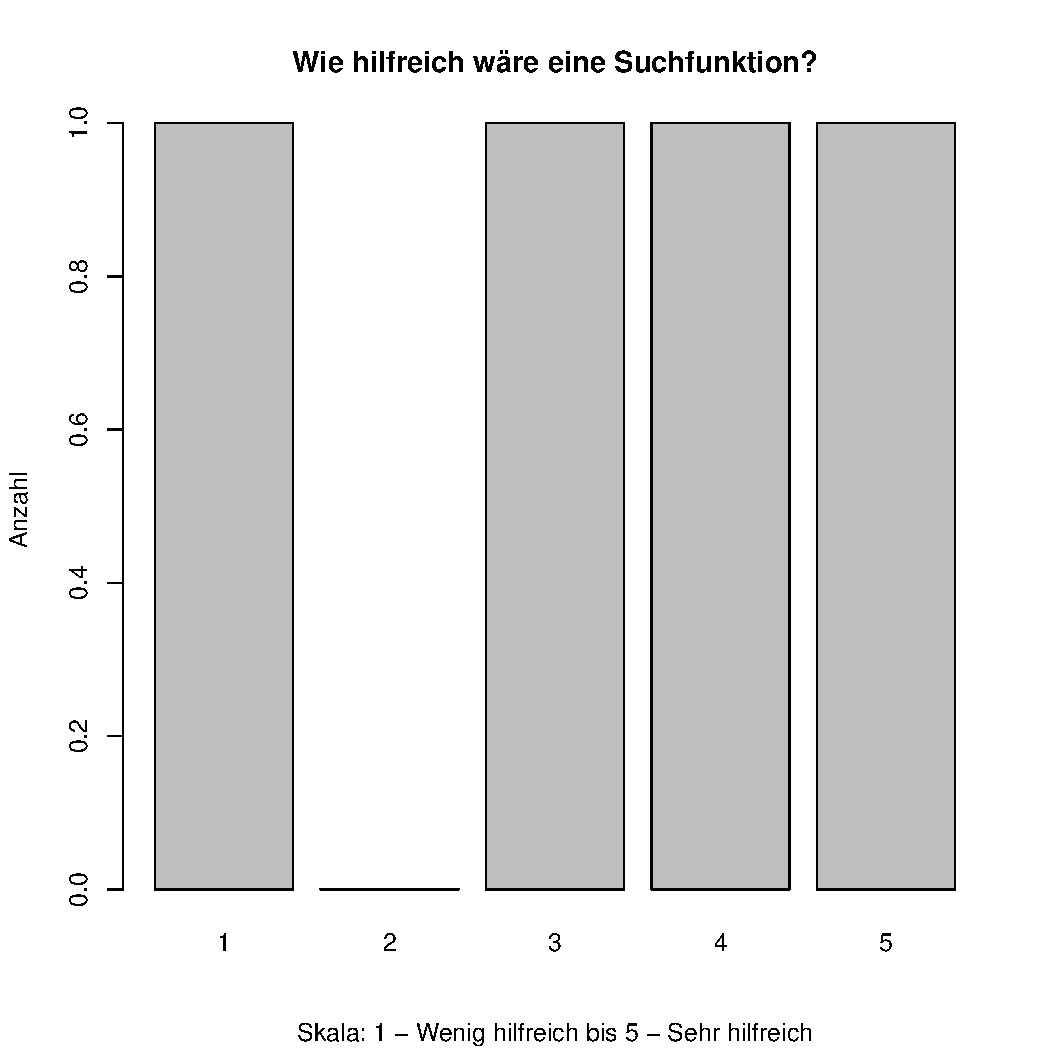
\includegraphics[width=0.60\textwidth]{q8-3.pdf}
    \caption{Nützlichkeit einer Suche}
	\label{fig:q83}
\end{figure} 
\subsubsection{Frage 8.4: Markieren}
\begin{figure}[H]
	\centering
	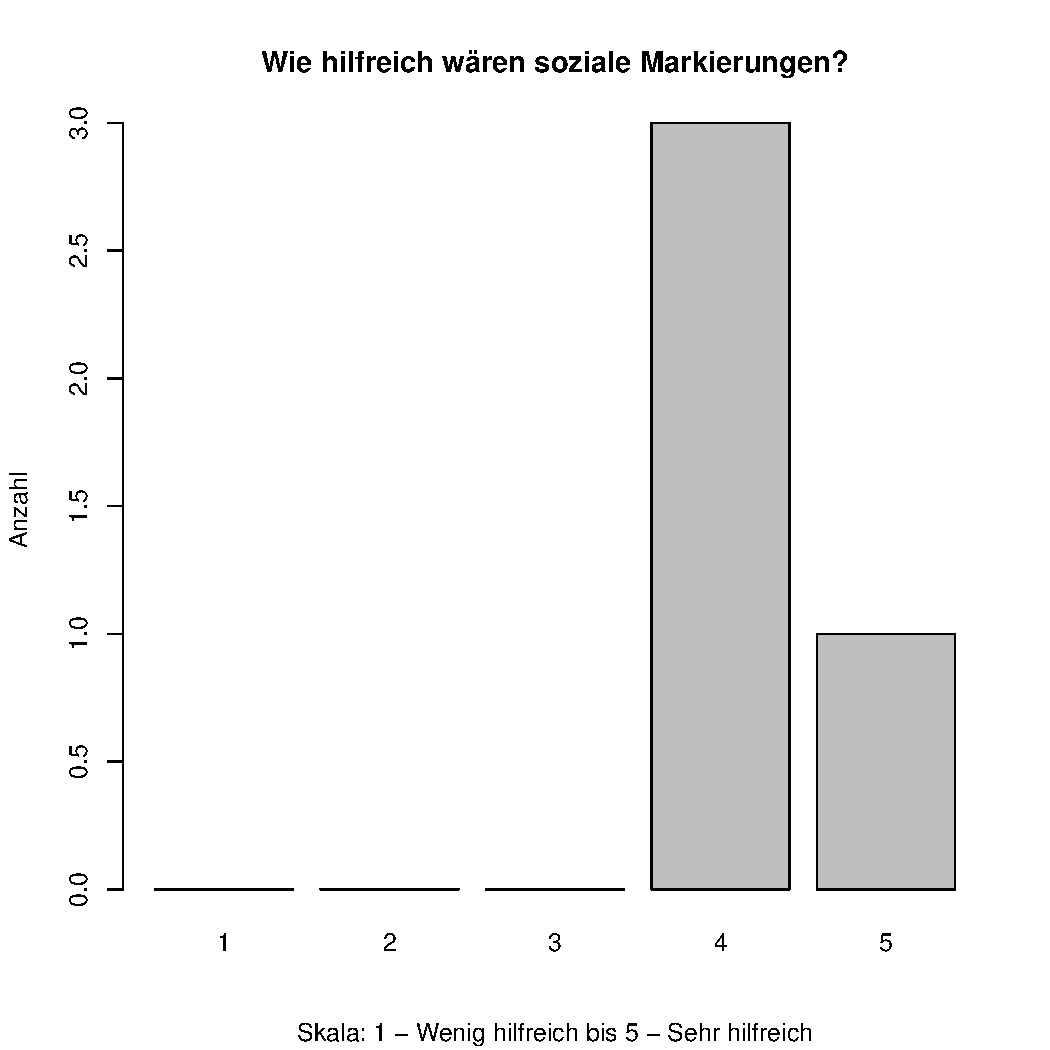
\includegraphics[width=0.60\textwidth]{q8-4.pdf}
    \caption{Nützlichkeit von Markierungen}
	\label{fig:q84}
\end{figure} 
\subsubsection{Frage 8.5: Vorgegebene Eingabefelder}
\begin{figure}[H]
	\centering
	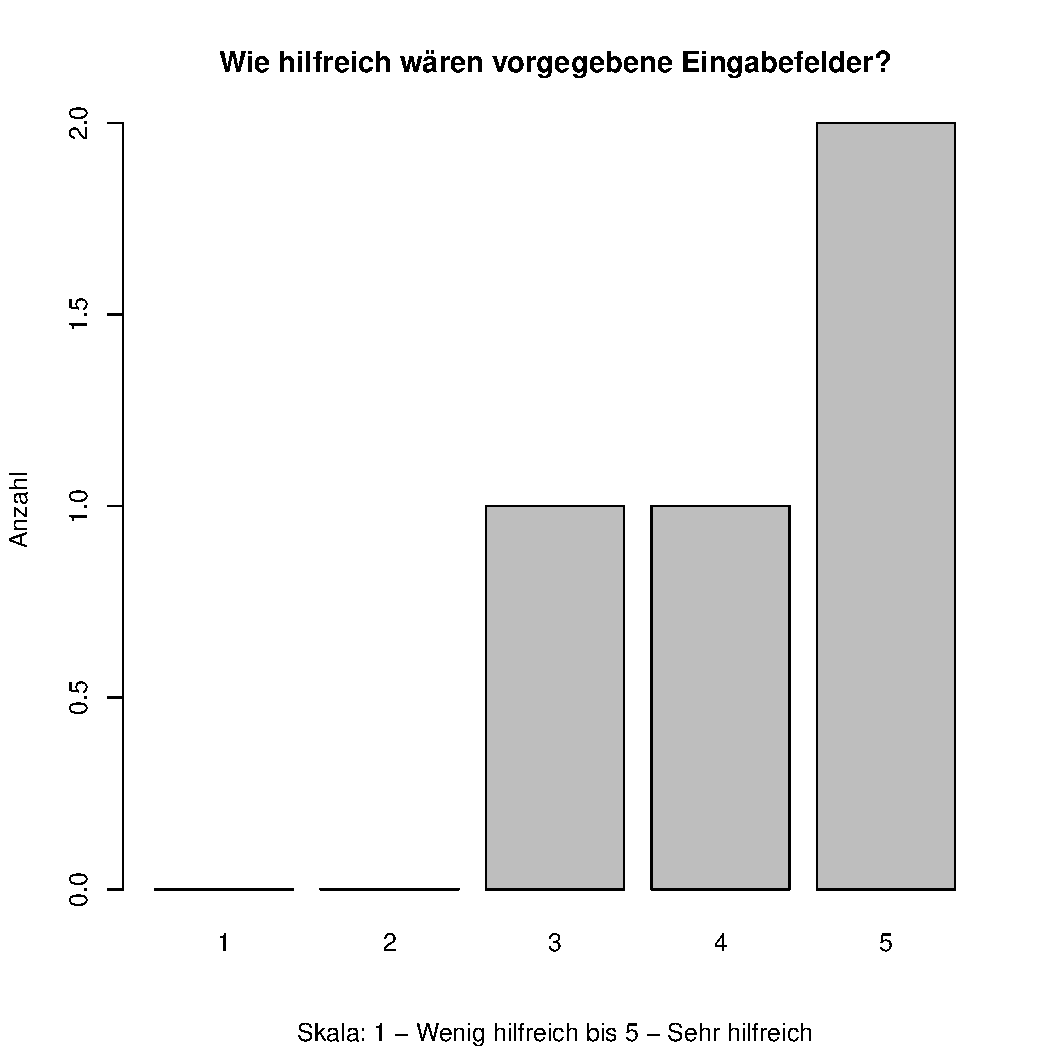
\includegraphics[width=0.60\textwidth]{q8-5.pdf}
    \caption{Nützlichkeit von Vorgaben}
	\label{fig:q85}
\end{figure} 
\subsection{Frage 9: Was ist dein bevorzugter Zeitpunkt für ein Weekly Standup?}
\begin{figure}[H]
	\centering
	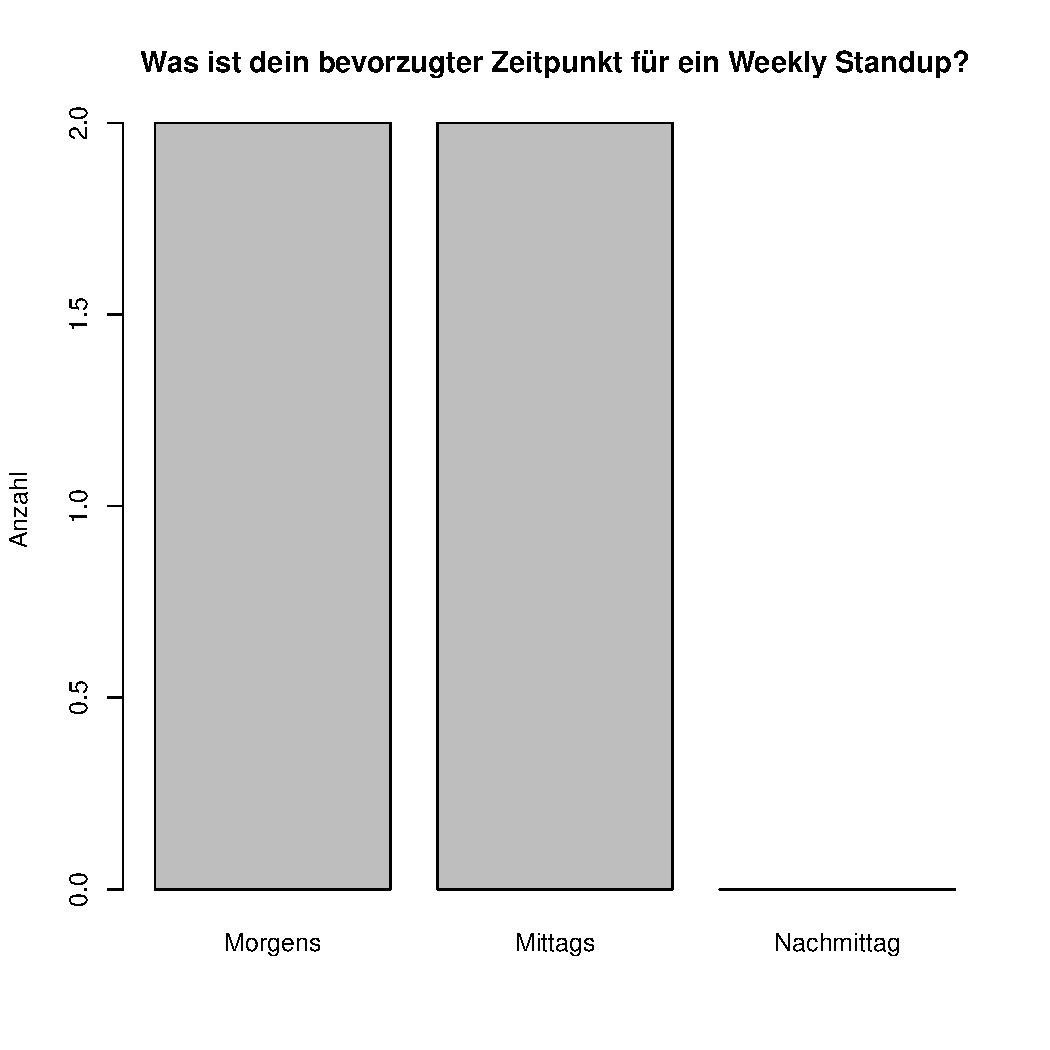
\includegraphics[width=0.60\textwidth]{q9.pdf}
    \caption{Idealer Zeitpunkt für ein Weekly Standup}
	\label{fig:q9}
\end{figure}  
\subsection{Frage 10: Welche Form eines Weekly Standups würdest du bevorzugen?}
\begin{figure}[H]
	\centering
	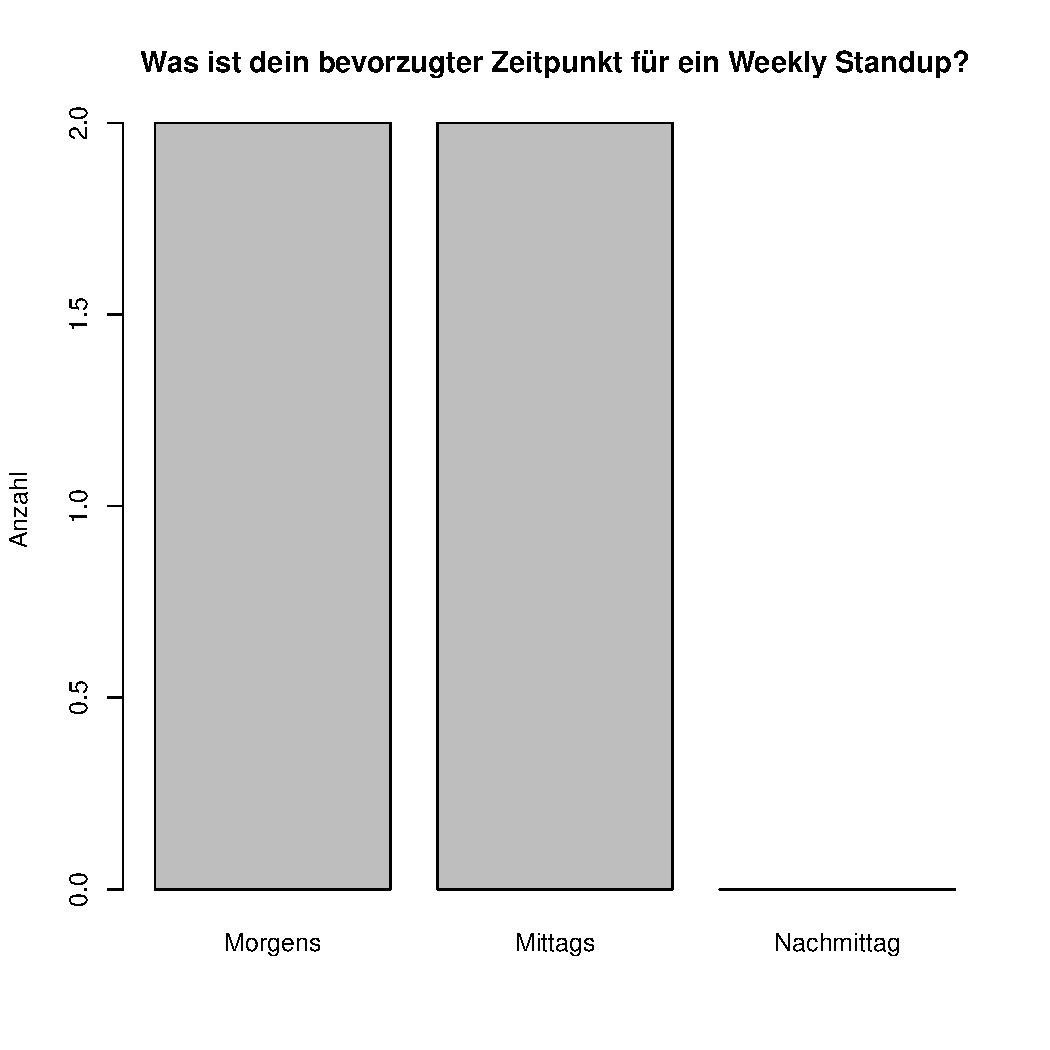
\includegraphics[width=0.60\textwidth]{q9.pdf}
    \caption{Bevorzugte form des Weekly Standups}
	\label{fig:q10}
\end{figure} 
\subsection{Frage 11: Würdest du einen Chatbot als hilfreich empfinden, welcher dir Informationen wie Deployment, Status, Logereignisse im Meeting mitteilt?}
\begin{figure}[H]
	\centering
	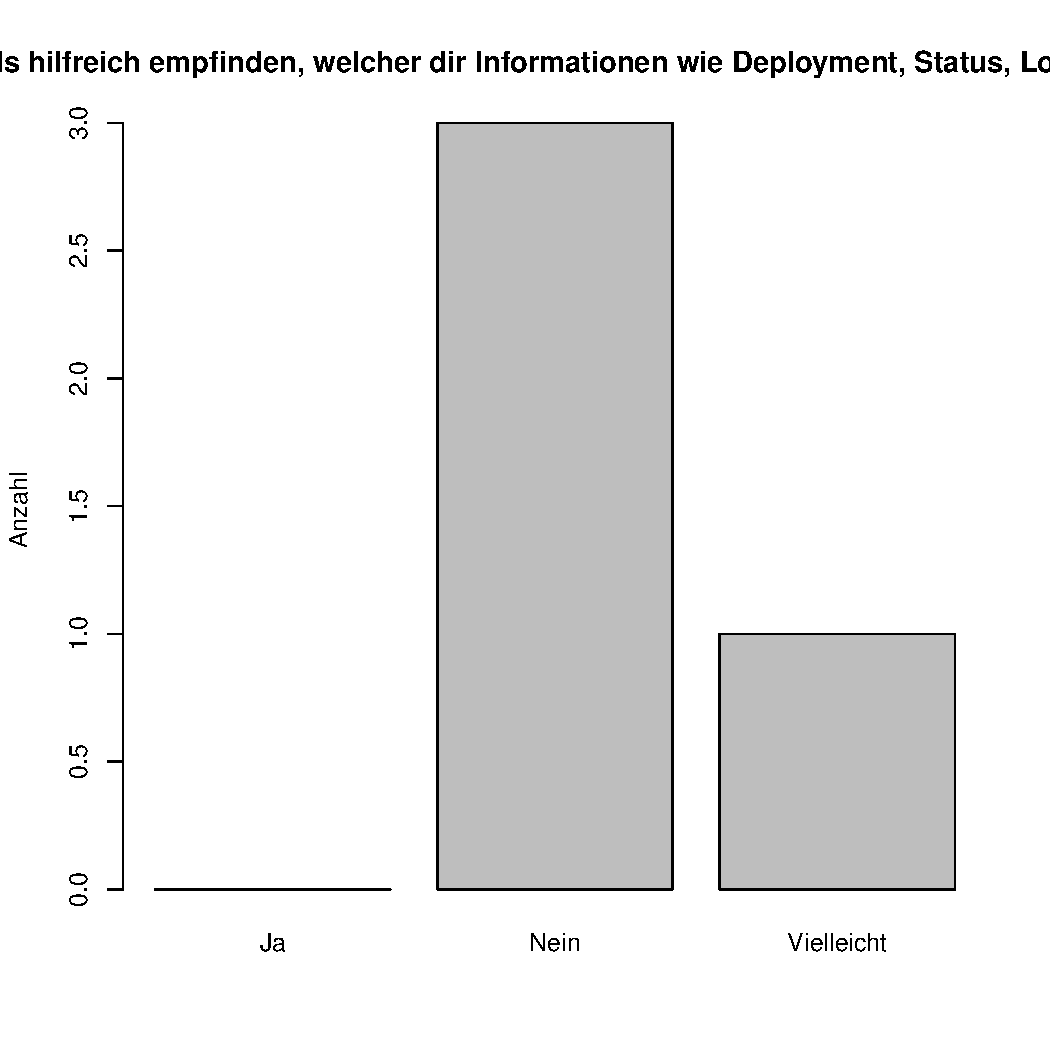
\includegraphics[width=0.60\textwidth]{q11.pdf}
    \caption{Meinung zu einem Chatbot}
	\label{fig:q11}
\end{figure} 
\subsection{Frage 12: Welche Informationen wären für dich als Projektmanager in einem Weekly Standup wichtig?}
Diese Frage wurde als Freitextaufgabe gestellt. Zwei der befragten haben sich dazu geäußert und folgende Informationen als wünschenswert zu erheben herausgestellt:
\begin{itemize}
\item Verknüpfung zu Aufgaben -> Überblick in Bezug auf den Plan
\item Muss ich als Dozent / PM intervenieren / Resourcen / Unterstützung / Hilfestellungen bereitstellen? 
\item Wer macht / wie viel mit? 
\item Gibt es Abwesenheiten?
\end{itemize}

\subsection{Frage 13: Wenn du bereits Weekly Standups gemacht hast, welche Tools hast du dafür benutzt?}
Bei dieser Frage handelte es sich wiederum um eine Freitext eingabe. die am häufigsten genannten Tools waren hierbei:
\begin{itemize}
    \item Jira (3x)
    \item Teams (3x)
    \item Miro
    \item Jitsi
\end{itemize}
Aber auch dinge wie Azure Devops oder digitale/smarte Whiteboards wurden genannt.

\subsection{Frage 14: Wie wichtig wäre dir eine Zeitbegrenzung des Meetings?}
\begin{figure}[H]
	\centering
	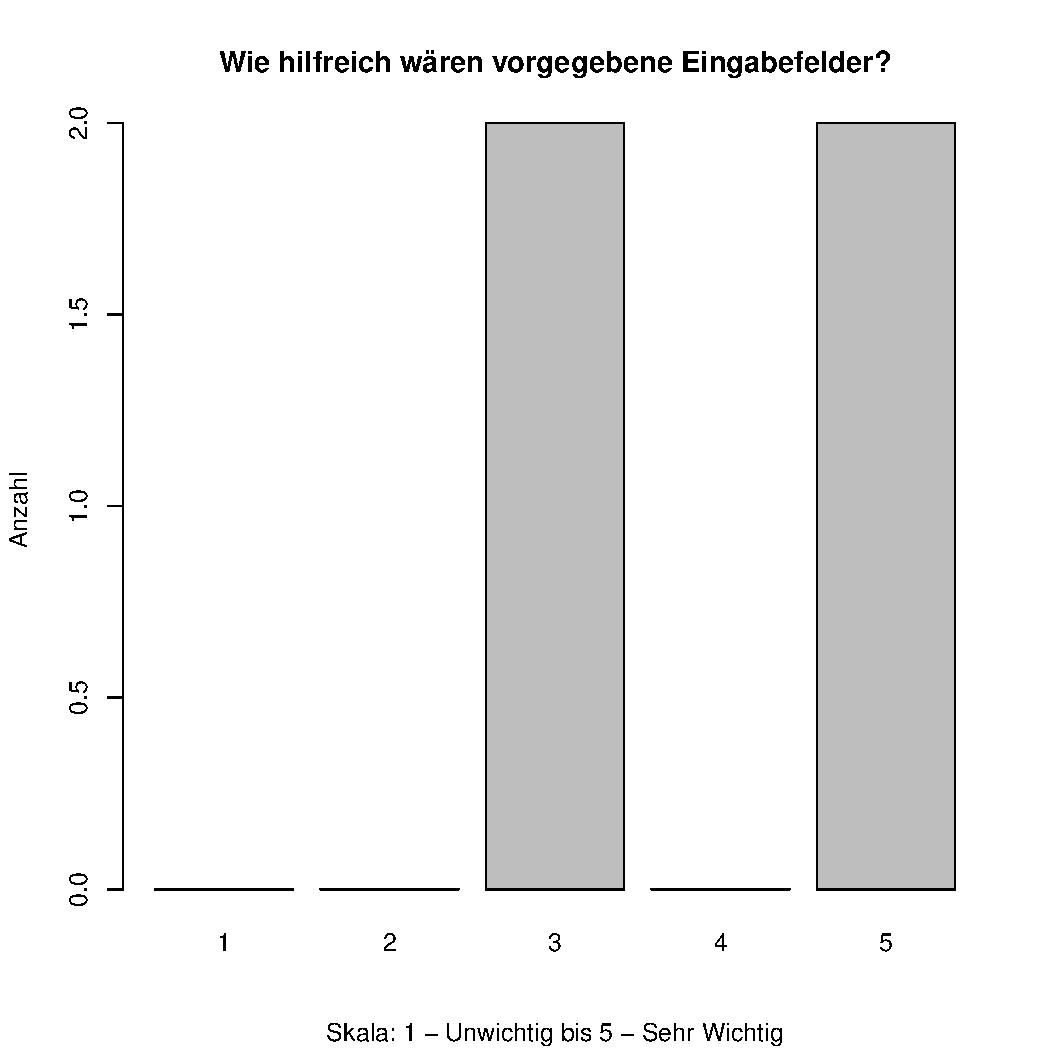
\includegraphics[width=0.60\textwidth]{q14.pdf}
    \caption{Wunsch nach Zeitbegrenzung}
	\label{fig:q14}
\end{figure} 
\section{Methodik}




	\chapter{User Stories}

Durch Brainstorming und Auswertung der Interviews haben wir folgende User Stories entwickelt

\section{Userstorymap}

\section{Glossar für die User Stories}
\begin{itemize}
\item \textbf{[MEETING]} : Eine Instanz eines Weekly Stand Ups
\item \textbf{[USER]} : Teilnehmer eines \textbf{[MEETING]}s 
\item \textbf{[PUNKT]} : Eine der drei möglichen Kategorien die Abgefragt werden (Was habe ich getan? Was werde ich tun? Was blockiert mich?)
\end{itemize}
\section{User Story Nr.1} 


Als \textbf{[USER]} möchte ich die Möglichkeit haben mit Mentions user oder meetings zu referenzieren

\section{User Story Nr.2}


Als \textbf{[USER]} möchte ich ein \textbf{[PUNKT]} markieren können (z.b.: ja, nein, lachen, traurig)
\section{User Story Nr.3}


Als \textbf{[USER]} möchte im \textbf{[MEETING]} die Teilnehmer und Datumsangaben sehen
\section{User Story Nr.4 }


Als \textbf{[USER]} möchte ich ein \textbf{[PUNKT]} bearbeiten oder löschen im aktuellen Meeting
\section{User Story Nr.5}


Als \textbf{[USER]} möchte ein Eingabefeld haben mit (Emojisupport) um meine \textbf{[PUNKT]}e einzutragen
\section{User Story Nr.6}


Als \textbf{[USER]} möchte ich einen \textbf{[PUNKT]} für das nächste \textbf{[MEETING]} eintragen
\section{User Story Nr.7}


Als \textbf{[USER]} möchte ich ein \textbf{[MEETING]} öffnen können um mehr Details erhalten
\section{User Story Nr.8}


als \textbf{[USER]} möchte ich vergangene \textbf{[MEETING]}s durchsuchen können (Schlagwortsuche)
\section{User Story Nr.9}


Als  \textbf{[USER]} möchte ich \textbf{[MEETING]}s starten können welche \textbf{[PUNKT]}e enthalten
\section{User Story Nr.10}


Als  \textbf{[USER]} möchte ich einfach durch die Timeline navigieren wo nur das aktive \textbf{[MEETING]} expanded ist
\section{User Story Nr.11}


Als \textbf{[USER]} möchte ich eine Liste von \textbf{[MEETING]} in einer Timeline sehen

\section{User Story Nr.12}

Als \textbf{[USER]} möchte ich ein  \textbf{[PUNKT]} als "wichtig" markieren
	\chapter{Risiko Analyse}

\section{Hintergrund}
Risikoanalysen dienen dazu vorhersehbaren Risiken zo erkennen, wenn möglich zu beheben und wenn nicht Möglich, wenigstens im Vorhinein zu identifizieren um besser darauf reagieren zu können. Die wesentlichen Schritte zu einer Risikoanalyse lassen sich wie folgt beschreiben.
\begin{figure}[H]
	\centering
	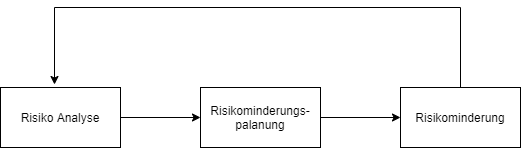
\includegraphics[width=0.8\textwidth]{risk-mitigation-loop}
    \caption{Risikoanalysezyklus \cite{osti_1494012}}
	\label{fig:r1}
\end{figure} 
\subsubsection{Risikoanalyse}
Während der Risikoanalysephase werden mögliche Risiken benannt und strukturiert erfasst und bewertet. Hierfür bieten sich mehrere Techniken an wie z.B das erstellen einer Risiko Matrix. Hierbei werden mögliche Risiken nach ihrer Schwere sowie ihrer Eintrittswahrscheinlichkeit kategorisiert. Ein Risiko welches eine sehr niedrige Eintrittswahrscheinlichkeit hat dafür aber nur sehr unwahrscheinlich eintritt kann unter Umständen akzeptabler sein als eines mit einem geringeren Impact aber einer hohen Eintrittswahrscheinlichkeit.
\begin{figure}[H]
	\centering
	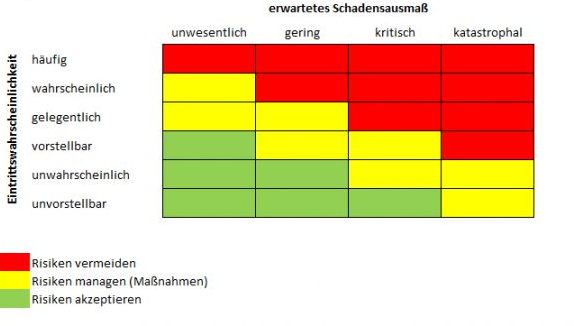
\includegraphics[width=0.8\textwidth]{risk-matrix}
    \caption{Beispiel für eine Risikomatrix \cite{risk2022}}
	\label{fig:r2}
\end{figure} 
\subsubsection{Risikominderungsplanung}
Bei der Risikominderungsplanung wird entschieden wie mit Risiken umgegangen werden soll. Hierbei wird für jedes erkannte Risiko entschieden wie mit ihm umgegangen wird. Mögliche Vorgehensweisen sind:
\begin{itemize}
    \item \textbf{Vermeiden:} Hierbei wird für das gefundene Risiko eine Lösung gefunden und damit das Risiko vermieden. Damit besteht kein weiteres Risiko von dem gefundenen Problem 
    \item \textbf{Verhindern:} Beim Verhindern werden Strategien erdacht, welche dazu führen ein Risiko weitest möglich auszuschließen. Ein gewisses Restrisiko besteht weiterhin und das gefundene Problem sollte in zukünftigen Zyklen weiterhin betrachtet werden. 
    \item \textbf{Akzeptieren:} Das Risiko wird so wie es ist akzeptiert und mit den Folgen wird gelebt. Auch diese Risiken sollten weiterhin verfolgt werden, da in Zukunft eine bessere Strategie für ihre Lösung vorhanden sein könnte.
\end{itemize}
\subsubsection{Risikoverhinderung}
In der Risikoverhinderungsphase werden erkannte Probleme anhand des Planes welcher zuvor erarbeitet wurde behoben.
\\
Abschließend kann wieder am ersten Schritt angefangen werden. Gerade in länger laufenden Projekten ist ein kontinuierliches Risikomanagement empfehlenswert, da sich Risiken im Laufe des Projektes verändern können.

\section{Risikoanalyse für das Projekt}
Aus den User stories und nach Rücksprache im Team haben wir die folgenden Risiken für das Projekt identifizieren können:

\begin{table}[ht]
    \centering
    \begin{adjustbox}{width=1\textwidth}
    \small
    \begin{tabular}{|l|l|l|l|}
    \hline
    Risiko & 
    Eintrittswahrscheinlichkeit & 
    Impakt  & 
    Strategie \\ 
    \hline
    Krankheit von Teammitgliedern 
    & Mittel - Hoch 
    & Hoch   
    & \tabitem Aufgaben verteilen \\
    &&&\tabitem Unabhängig voneinander arbeiten \\ 
    \hline
    Integration in SPMS schwieriger als gedacht 
    & Niedrig - Mittel 
    & Mittel 
    & \tabitem Proaktiv auf Hr. Schulz zugehen \\
    &&&\tabitem Frühzeitig testen           \\ 
    \hline
    Kommunikation mit Dozent schwierig                 
    & Niedrig 
    & Niedrig 
    & Proaktiv auf Dozentin zugehen\\ \hline
    Erwartung der Test User nicht erfüllt
    & Niedrig                     
    & Hoch    
    & \tabitem Nutzer frühzeitig involvieren \\
    &&&\tabitem Feedback einholen \\
    &&&\tabitem Fragebogen         
    \\ \hline
    Zeitlicher Aufwand unterschätzt                     
    & Mittel                      
    & Hoch    
    & \tabitem Möglichst genau Planen \\
    &&&\tabitem Erfahrung von Teammitgliedern nutzen \\ \hline
    Aufwand der Implementierung aller Features zu hoch & Mittel                      
    & Mittel  
    & Abestufte Funktionalität einplanen                            
    \\ \hline
    Atomkrieg mit anschließender Zombieapokalypse      
    & ... hoffentlich niedrig?    
    & Hoch    
    & Duck \& Cover \\ \hline
    \end{tabular}%    
\end{adjustbox}
    \caption{Risikoanlyse des Projekts}
    \label{tab:risk-table}
    \end{table}

Aufgrund der überschaubaren Risiken haben wir eine kombinierte Darstellung aus erkannten Risiken, ihren Eintrittswahrscheinlichkeiten und ihrer Lösung, sofern vorhanden, gewählt. Je nach Größe oder Kritikalität eines Projektes können sich separate Darstellungen oder gar Dokumente besser eignen da sie unter Umständen hunderte Risiken enthalten können.
	\chapter{Projektplan}
	\chapter{Implementierung}
	\chapter{Mögliche Erweiterungen}

Wir haben uns noch mehre weitere Features für unsere \ac{SPMS} Erweiterung in Planung gehabt aber aus Zeitmangel erstmal hinten angestellt.

\section{Aufgabenplanung}

Ein (auch in den Interviews) genanntes Feature wäre eine Verknüpfung zu einer Aufgabenveraltung. Dies könnte man mit zwei Features erreichen

\subsection{Kanban Board}

Das \ac{SPMS} könnte für die Projekte über ein Kanban Board erweitert werden. Auf diesem Board können die Studenten auf eine einfache Art und Weise Aufgaben anlegen und einem verantwortlichen zugewiesen werden.

\subsection{Aufgaben Verküpfung}

Im Weekly Standup könnte man dann eine Aufgabe direkt referenzieren zum Beispiel durch ein vorangestelltes "§". Gibt man ein "§" werden einem aufgaben aus dem Kanban Board vorgeschlagen
	\clearpage

%%%%% Bibliography
	\fancyhead[LE,RO]{\nouppercase\leftmark}
	\printbibliography[heading=bibintoc]
	\cleardoublepage
%%%%% Appendix
	\fancyhead[LE,RO]{A  \ -- \ \nouppercase\leftmark}
	\begin{appendices}
\chapter{Appendix}
\pagebreak

\begin{figure}[H]
	\centering
	 \caption{A Big Image}
	\includegraphics[width=0.95\textwidth]{example-image.pdf}
	\label{fig:appendixImage}
\end{figure}

\begin{lstlisting}[caption={Fibonacci}, label={lst:fibAppendix}, captionpos=t]
public class Fibonacci {
	public static long fib(int n) {
		if (n <= 2) {
			return 1;
		} else {
			return fib(n - 1) + fib(n - 2);
		}
	}

	public static void main(String[] args) {
		for(int i = 1; i < 10; i++) {
			System.out.println(i + " - " + fib(i));
		}
	}
}
\end{lstlisting}
\end{appendices}

\end{document}
